\documentclass[12pt, a4paper, oneside]{CIITThesissV1}
\usepackage{placeins}
\usepackage{multirow}
\usepackage{sectsty}
\usepackage{graphicx}
\usepackage{graphics}
\usepackage[table]{xcolor}
\usepackage{lscape}
\usepackage[autostyle]{csquotes}
\usepackage{amsfonts}
\usepackage{amstext}
\usepackage{amssymb}
\usepackage[english]{babel}
\usepackage{parskip}
\usepackage[export]{adjustbox}
\usepackage{pbox}


\usepackage{threeparttable}  
\usepackage{booktabs}
\usepackage{multirow}
\usepackage{bm}


\usepackage{hhline}%%%
\usepackage{pdfpages}
\usepackage{rotating}
\usepackage{epsfig}
\usepackage{booktabs}
\usepackage{float}
\usepackage{url}
\usepackage{nomencl}
\usepackage{amsmath}
\usepackage[utf8]{inputenc}
\usepackage{xcolor}
\usepackage{color, colortbl}
\usepackage{lipsum}
\usepackage{setspace}
\usepackage{afterpage}
\usepackage{pdflscape}
\usepackage{pstricks}
%\usepackage{subfigure}
\usepackage{titlesec}
\usepackage{cases}
\usepackage{tocloft}
\usepackage[numbers]{natbib}
\usepackage{amsmath}
\usepackage[hypcap=false]{caption}
\usepackage{authblk}
\usepackage{rotating}
\usepackage{pifont}
\usepackage{url}
\usepackage{array}
\usepackage{enumitem}
\usepackage{bookmark}
\usepackage{arydshln}
\usepackage{booktabs}
\usepackage{amsmath,amssymb,amsfonts}
%\usepackage[ruled,linesnumbered]{algorithm2e}
%The following line is added to support the algorithms.
\usepackage[ruled,vlined]{algorithm2e}
\usepackage{graphicx}
\usepackage{subcaption}
\usepackage{hyperref}
%\usepackage{longtable}
\usepackage[toc,page]{appendix}
\usepackage{matlab}
\usepackage{listings}
\lstset{breaklines=true}
\usepackage{lineno}
\usepackage{mfirstuc}


\usepackage{pdflscape} % For landscape orientation
\usepackage{xltabular} % Extended tabular with auto page break and X columns
\usepackage{booktabs} % For better table formatting
\usepackage[table]{xcolor} % For cell coloring
\usepackage{makecell} % For line breaks within cells
\usepackage{listings} % For including code-like listings
\usepackage{xcolor} % For color definitions in listings

\makeatletter
\def\BState{\State\hskip-\ALG@thistlm}
\graphicspath{{figures/}}
\makeatother

\renewcommand\cftchapfont{\textbf\normalfont}
\renewcommand\cftchappagefont{{\normalfont}}
\AtBeginDocument{\renewcommand\contentsname{TABLE OF CONTENTS}}
%\AtBeginDocument{\renewcommand\contentsname{\leftline{LIST OF FIGURES}}}
\titleformat{\chapter}[display]
{\bfseries\Large}
{\vspace{4cm}\centering\bigskip \Large\bfseries{Chapter \thechapter}}
{1ex}
{\bfseries\Large\centering}

\begin{document}
\pagenumbering{roman}

\begin{center}

\LARGE \capitalisewords {A Novel Testing Framework for Vision Models Using Bayesian Network}

\end{center}

\begin{center}
%\begin{figure}
	
\includegraphics[width=6cm]{nu_logo.jpeg}
%\end{figure}
\end{center}
\begin{center}
\emph{\large By}\\

\Large {\href{https://scholar.google.com/citations?hl=en&user=ZEwBUxwAAAAJ&view_op=list_works&authuser=1&gmla=AILGF5XqzU9IqXxSuitd8SwCxQWSLHy9OoSQ59cgiyOt3Pi35gv5n8bJg_gLqFhg9SZZv2U2fvQ7DMDOmR6oiGnT5TQkhZ-vwzUvrJNRPEY2m2XMukSMolIK07cvFv6HJGZ6fEN2UhAmB9NIRd1pNy95LBWH7vzvwukF9plB9Ag}{\color{blue} Arooj Arif}}\\
\Large aa3506phd\
\vfill
\Large Mini-thesis is submitted for the probation review of PhD\\
\Large July 2024\\
% \Large Computer Science
\end{center}
\vfill

\begin{center}
\Large Northeastern University London, London - UK
\end{center}

\begin{center}
\LARGE Spring, 2024
\end{center} 
\thispagestyle{empty}
% \begin{minipage}{0.1\textwidth}
% 
\includegraphics[scale=0.2]{ciitlogo.png}
  
\includegraphics[width=1cm]{nu_logo.jpeg}
\end{minipage}
\begin{minipage}{0.7\textwidth}\raggedleft
\textbf{\Large Northeastern University London}
\end{minipage}
\vfill
\vfill
\begin{center}

\LARGE \capitalisewords {A Novel Testing Framework for Vision Models Using Bayesian Network}

\end{center}

\vfill
\begin{center}\large
A Mini-thesis Presented to\\
\vfill
\Large Northeastern University London
\end{center}

\vfill
\begin{center}\normalsize
In partial fulfillment\\
of the requirement for the degree of
\end{center}

\begin{center}\LARGE
Phd (Computer Science)
\end{center}

\vfill
\begin{center}


\normalsize By\\

\large Arooj Arif\\
\large aa3506phd\\
\end{center}
\vfill


\begin{center}
\Large Spring, 2024
\end{center}

% 
\begin{center}

\LARGE \capitalisewords {A Novel Testing Framework for Vision Models Using Bayesian Network}

\end{center}
\noindent\rule{15.5cm}{3pt}\\

\normalsize
A Post Graduate Thesis submitted to the Department of Computer Science as partial fulfilment of the requirement for the award of Degree of Phd (Computer Science).
\vfill
\begin{center}
\begin{table}[ht]
\centering
%\begin{tabular}{| >{\centering}b{2.3in} | c |}

\begin{tabular}{|l |l |}
\hline \noalign{\hrule height 2pt}
{\fontsize{16}{15} \normalfont } & {\fontsize{16}{15} \normalfont } \\
{\fontsize{16}{15} \normalfont Name} & {\fontsize{16}{15} \normalfont  Registration Number} \\ \hline
& \\
{\fontsize{16}{15} \normalfont Arooj Arif} & {\fontsize{16}{15} \normalfont aa3506phd}\\[2ex] \noalign{\hrule height 2pt}
\end{tabular}
\end{table}
\end{center}
\noindent \textbf{\large Supervisor:}
\vfill
\normalsize
\noindent \href{https://scholar.google.co.uk/citations?user=kQr7ip4AAAAJ&hl=en}{\color{blue} Dr Alexandros Koliousis}, \\
Associate Professor, Department of Computer Science,\\
Northeastern University,\\
London, UK\\
\noindent \textbf{\large Co-Supervisor:}
\vfill
\normalsize
\noindent \href{https://scholar.google.co.uk/citations?user=fEkC0gkAAAAJ&hl=en}{\color{blue}Elena Botoeva}, \\
Lecturer, Department of Computer Science,\\
University of Kent,\\
Kent, UK
\vfill



\begin{center}

\Large Final Approval
\end{center}
\noindent\rule{15.5cm}{3pt}

\begin{center}
\normalsize
 This Mini-thesis titled\\
\end{center}


\begin{center}
\large \capitalisewords {TestifAI: A Comprehensive Testing Framework for Safe AI}
\end{center}

\vfill
\begin{center}
By\\
\emph{Arooj Arif\\
aa3506phd}
\end{center}


\begin{center}\normalsize
has been approved\\
For the Northeastern University, London
\end{center}

%\vfill
%\vfill
%
%\normalsize
%External Examiner:\line(10,0){295}
%\vspace{-0.50cm}
%\begin{center}\normalsize
%	Dr. Imtiaz Ahmad Taj\\
%	Professor, Dean Faculty of Engineering,\\
%	Capital University of Science \& Technology (CUST), Islamabad
%\end{center}


\vfill
\normalsize
Chair:\line(10,0){285}
\vspace{-0.50cm}
\begin{center}\normalsize
    Alex Freitas,\\
    Professor, Department of Computer Science,\\
    University of Kent, Kent\\

\end{center}

\vfill
\normalsize
Supervisor:\line(10,0){285}
\vspace{-0.50cm}
\begin{center}\normalsize
Alexandros Koliousis,\\
Associate Professor, Department of Computer Science,\\
Northeastern University London, UK
\end{center}

\vfill
\normalsize
Co-Supervisor:\line(10,0){285}
\vspace{-0.50cm}
\begin{center}\normalsize
Elena Botoeva, \\
Lecturer, Department of Computer Science,\\
University of Kent, Kent
\end{center}


\vfill
\vfill

% \normalsize
% Head of Department:\line(10,0){295}
% \vspace{-0.50cm}
% \begin{center}\normalsize
% abc,\\
% Abc,\\
% ABC
% \end{center}



% %%% DECLARATION %%%%
%%%%%%%%%%%%%%%%%%%
\vspace{2in}
\begin{center}
{\large \bf Declaration}\\
\end{center}

\vspace{0.7cm}
\normalsize
I \underline{Arooj Arif (Registration No. aa3506phd)} hereby declare that I have produced the work presented in this thesis, during the scheduled period of study. I also declare that I have not taken any material from any source except referred to wherever due that amount of plagiarism is within acceptable range. 
% If a violation of HEC rules on research has occurred in this thesis, I shall be liable to punishable action under the plagiarism rules of the HEC.

\vspace{1in}

\begin{table}[ht]
\centering
\begin{tabular}{ l  p{1.5in} c}
Date: \underline{July, 2024} & & \line(10,0){150} \\
& & Arooj Arif \\
& & aa3506phd \\
\end{tabular}
\end{table}

\clearpage
\newpage

% \clearpage
\newpage
%%% CERTIFICATE %%%%
%%%%%%%%%%%%%%%%%%%%
\vspace{2in}
\begin{center}
{\large \bf Certificate}\\
\end{center}

\vspace{0.7cm}
\normalsize
It is certified that \underline{Arooj Arif (Registration No. aa3506phd)} has carried out all the work related to this thesis under my supervision at the Department of Computer Science, Northeastern University, London and the work fulfils the requirement for award of Phd degree.

\vspace{1in}

\begin{table}[ht]
\centering
\begin{tabular}{ l  p{0.01in} c}
Date: \underline{July, 2021} & & \\
& & \\
& & \\
& & \hspace{-4.5cm} Supervisor: \\
\\
\\
& & \hspace{-0.5cm} \line(10,0){175}\\
& & \hspace{-0.5cm} Dr. Alexandros Koliousis\\
& & \hspace{-0.5cm} Associate Professor, Department of Computer Science \\
& & \\
& & \\
& & \\
& & \\
& & \hspace{-4.5cm} Co-Supervisor: \\
\\
\\
& & \hspace{-0.5cm} \line(10,0){175}\\
& & \hspace{-0.5cm} Dr. Elena Botoeva\\
& & \hspace{-0.5cm} Lecturer, Department of Computer Science\\
%Higher Colleges of Technology, Fujairah, United Arab Emirates


Head of Department: & & \\
\\
\\
\line(10,0){175} & & \\
Dr.Abc & & \\
Department of Computer Science & & \\
\end{tabular}
\end{table}

\clearpage
\newpage

% 
%DEDICATION PAGE

\addcontentsline{toc}{chapter}{Dedication}
\vspace{0.7cm}
\begin{center}
{\fontsize{16}{15} \bf DEDICATION}\\
\end{center}

\vspace{1cm}
\begin{center}
  \large{ { {\Huge $\mathcal{D}$}edicated

	to my mentor Dr. Alexandros Koliousis and loving Parents, who equipped me with pearls of knowledge and showed me the way of spiritual and personal enlightenment in this world and the world hereafter. \\
      } }
\end{center}
\clearpage
\newpage

% 
%ACKNOWLEDGEMENTS PAGE

\addcontentsline{toc}{chapter}{Acknowledgements}
\vspace{0.7cm}
\begin{center}
{\fontsize{16}{15} \bf ACKNOWLEDGEMENT}\\
\end{center}
\vspace{0.7cm}
% \normalsize First of all, thanks to Allah Almighty who give me strength and confidence to complete this dissertation. After that, I would like to express my profound appreciation to many people who supported me
% during my MS and who helped me to complete my thesis. Their generous support
% made this research work possible
% \par

% Firstly, I would like to express my sincere gratitude to my advisor Dr. Nadeem Javaid for the continuous support of my MS study and related research, for his patience, motivation and immense knowledge. His guidance helped me in all the time of research and writing of this thesis. I could not have imagined having a better advisor and mentor for my MS study. I am truly indebted to him for his knowledge, thoughts and friendship.\par
% I would like to thank my parents for their continuous support, understanding and assistance whenever I needed them throughout my MS studies and research work. Furthermore, I would like to thank my brothers Mohammad Jamal, Ahmed Jamal and Qasim Jamal. I believe that without their motivation, it is not possible to succeed throughout my life. I am always grateful to them for their encouragement and support.
% \par
% Last but not the least, I am greatly thankful to Director of ComSens Lab and all of my colleagues at CUI for providing me the warm and friendly atmosphere.
\clearpage
\newpage

% $Log: abstract.tex,v $
% Revision 1.1  93/05/14  14:56:25  starflt
% Initial revision
% 
% Revision 1.1  90/05/04  10:41:01  lwvanels
% Initial revision
% 
%
%% The text of your abstract and nothing else (other than comments) goes here.
%% It will be single-spaced and the rest of the text that is supposed to go on
%% the abstract page will be generated by the abstractpage environment.  This
%% file should be \input (not \include 'd) from cover.tex.
In this thesis, I designed and implemented a compiler which performs
optimizations that reduce the number of low-level floating point operations
necessary for a specific task; this involves the optimization of chains of
floating point operations as well as the implementation of a ``fixed'' point
data type that allows some floating point operations to simulated with integer
arithmetic.  The source language of the compiler is a subset of C, and the
destination language is assembly language for a micro-floating point CPU.  An
instruction-level simulator of the CPU was written to allow testing of the
code.  A series of test pieces of codes was compiled, both with and without
optimization, to determine how effective these optimizations were.

% \addcontentsline{toc}{chapter}{Conference Proceedings}

\begin{center}
	%{{\fontsize{16}{15} \bf ABSTRACT}\\}
	{\fontsize{16}{15} \bf Conference Proceedings \\ \vspace{0.3cm}
		}
	\vspace{0.4cm}
\end{center}
\normalsize
\begin{itemize}
\item[1] Muhammad Umar Javed, \underline{\textbf{Abid Jamal}}, Nadeem Javaid, Noman Haider, and Muhammad Imran. "Conditional Anonymity enabled Blockchain-based Ad Dissemination in Vehicular Ad-hoc Network." In 2020 International Wireless Communications and Mobile Computing (IWCMC), pp. 2149-2153. IEEE, 2020. {\href{https://ieeexplore.ieee.org/abstract/document/9148487}{Download}}

\item[2] Affaf Shahid, Umair Sarfraz, Muhammad Waseem Malik, Muhammad Sohaib Iftikhar, \underline{\textbf{Abid Jamal}} and Nadeem Javaid, "Blockchain-Based Reputation System in Agri-Food Supply Chain", Advanced Information Networking and Applications. AINA 2020. Advances in Intelligent Systems and Computing, vol 1151. Springer, 2020. {\href{https://link.springer.com/chapter/10.1007/978-3-030-44041-1_2}{Download}}

\item[3] Asad Ullah Khan, Affaf Shahid, Fatima Tariq, Abdul Ghaffar, \underline{\textbf{Abid Jamal}}, Shahid Abbas and Nadeem Javaid, "Enhanced Decentralized Management of Patient-Driven Interoperability Based on Blockchain",Advances on Broad-Band Wireless Computing, Communication and Applications. BWCCA 2019. Lecture Notes in Networks and Systems, vol 97. Springer, 2019. {\href{https://link.springer.com/chapter/10.1007/978-3-030-33506-9_74}{Download}}

\item[4] \underline{\textbf{ Abid Jamal}}, Sana Amjad, Usman Aziz, Muhammad Usman Gurmani, Saba Awan and Nadeem Javaid, "A Privacy Preserving Hybrid Blockchain based Announcement Scheme for Vehicular Energy Network", in the 15th International Conference on Complex, Intelligent and Software Intensive System (CISIS), 2021, ISBN: 978-3-030-50454-0.
{\href{https://www.researchgate.net/publication/351133979_A_Privacy_Preserving_Hybrid_Blockchain_based_Announcement_Scheme_for_Vehicular_Energy_Network}{Download}}

\item[5] \underline{\textbf{Abid Jamal}}, Muhammad Usman Gurmani, Saba Awan, Maimoona Bint E Sajid, Sana Amjad and Nadeem Javaid, "Blockchain enabled Secure and Efficient Reputation Management for Vehicular Energy Network", in the 15th International Conference on Complex, Intelligent and Software Intensive System (CISIS), 2021, ISBN: 978-3-030-50454-0.
{\href{https://www.researchgate.net/publication/351133976_Blockchain_enabled_Secure_and_Efficient_Reputation_Management_for_Vehicular_Energy_Network}{Download}}


\end{itemize}
\clearpage
\newpage 
% \addcontentsline{toc}{chapter}{Conference Proceedings}

\begin{center}
	%{{\fontsize{16}{15} \bf ABSTRACT}\\}
	{\fontsize{16}{15} \bf Conference Proceedings \\ \vspace{0.3cm}
		}
	\vspace{0.4cm}
\end{center}
\normalsize
% \begin{itemize}
	

% \item[1] \underline{\textbf{Abid Jamal}}, Sana Amjad, Usman Aziz, Muhammad Usman Gurmani, Saba Awan and Nadeem Javaid, "A Privacy Preserving Hybrid Blockchain based Announcement Scheme for Vehicular Energy Network", in the 15th International Conference on Complex, Intelligent and Software Intensive System (CISIS), 2021, ISBN: 978-3-030-50454-0.
% {\href{https://link.springer.com/chapter/10.1007/978-3-030-79725-6_14}{Download}}

% \item[2] \underline{\textbf{Abid Jamal}}, Muhammad Usman Gurmani, Saba Awan, Maimoona Bint E Sajid, Sana Amjad and Nadeem Javaid, "Blockchain enabled Secure and Efficient Reputation Management for Vehicular Energy Network", in the 15th International Conference on Complex, Intelligent and Software Intensive System (CISIS), 2021, ISBN: 978-3-030-50454-0.
% {\href{https://link.springer.com/chapter/10.1007/978-3-030-79725-6_40}{Download}}



% \item[3] Muhammad Umar Javed, \underline{\textbf{Abid Jamal}}, Nadeem Javaid, Noman Haider, and Muhammad Imran. "Conditional Anonymity enabled Blockchain-based Ad Dissemination in Vehicular Ad-hoc Network." In 2020 International Wireless Communications and Mobile Computing (IWCMC), pp. 2149-2153. IEEE, 2020. {\href{https://ieeexplore.ieee.org/abstract/document/9148487}{Download}}

% \item[4] Affaf Shahid, Umair Sarfraz, Muhammad Waseem Malik, Muhammad Sohaib Iftikhar, \underline{\textbf{Abid Jamal}} and Nadeem Javaid, "Blockchain-Based Reputation System in Agri-Food Supply Chain", Advanced Information Networking and Applications. AINA 2020. Advances in Intelligent Systems and Computing, vol 1151. Springer, 2020. {\href{https://link.springer.com/chapter/10.1007/978-3-030-44041-1_2}{Download}}

% \item[5] Asad Ullah Khan, Affaf Shahid, Fatima Tariq, Abdul Ghaffar, \underline{\textbf{Abid Jamal}}, Shahid Abbas and Nadeem Javaid, "Enhanced Decentralized Management of Patient-Driven Interoperability Based on Blockchain",Advances on Broad-Band Wireless Computing, Communication and Applications. BWCCA 2019. Lecture Notes in Networks and Systems, vol 97. Springer, 2019. {\href{https://link.springer.com/chapter/10.1007/978-3-030-33506-9_74}{Download}}



% \end{itemize}
\clearpage
\newpage 
  % -*- Mode:TeX -*-
%% This file simply contains the commands that actually generate the table of
%% contents and lists of figures and tables.  You can omit any or all of
%% these files by simply taking out the appropriate command.  For more
%% information on these files, see appendix C.3.3 of the LaTeX manual.
\setcounter{secnumdepth}{5}
\tableofcontents
\let\cleardoublepage\clearpage
\newpage
%\listoffigures
%let\cleardoublepage\clearpage
%\newpage
%\listoftables
%\let\cleardoublepage\clearpage
%\newpage
%\listofalgorithms
%\let\cleardoublepage\clearpage



\addcontentsline{toc}{chapter}{List of Figures}
\listoffigures
\clearpage

\addcontentsline{toc}{chapter}{List of Tables}
\listoftables 
\clearpage
\addcontentsline{toc}{chapter}{List of Algorithms}
\listofalgorithms
\clearpage
% \addcontentsline{toc}{chapter}{List of Symbols}
\chapter*{List of Abbreviations and Symbols}
%\markright{List of Symbols}

\begin{longtable}{ l l}

% J1 Symbols

% BC & Blockchain \\
% RSU & RoadSide Unit \\
% ITS & Intelligent Transport System \\ 
% MANET & Mobile Ad-hoc Network \\
% V2V & Vehicle to Vehicle \\ 
% V2I & Vehicle to Infrastructure \\ 
% OBU & On-Board Unit \\ 
% DSRC & Dedicated Short-Range Communication \\ 
% SPoF & Single Point of Failure \\ 
% DLT & Distributed Ledger Technology \\ 
% ECC & Elliptic Curve Cryptography \\
% P2P & Peer to Peer \\ 
% CA	& Certificate Authority		\\
% ECDSA	& Elliptic Curve Digital Signature Algorithm	\\
% PoAR & Proof of Ad Receiving \\
% CF  & Cuckoo Filter \\
% IPFS & Interplanetary Filesystem \\
% SSS & Shamir Secret Sharing \\


% $V_{s}$ & Ad sender vehicle \\
% $V_{r}$ & Ad receiving vehicle \\

% $G$ & Generator of elliptic group \\
% $h$ & Number of Ad fragments \\
% $PK$ & Public Key \\
% $PR$ & Private Key (Secret Key) \\
% $Sig$ & Digital Signature \\
% $Cert$ & Pseudonym Certificate \\
% $Link$ & Linkability between RID and PID\\
% $M$ & Ad message\\
% $TI$ & deadline (Time Threshold)\\

% %J2 symbols

% $MSK$ & Master Secret Key \\ 
% $MPK$ & Master Public Key \\ 
% $RevKey$ & Revocation Key \\ 
% $RID$ & Real Identity \\ 
% $PID$ & Pseudonym Identity \\ 
% $ts$ & Timestamp \\ 
% $TxReq$ & Request Transaction \\ 
% $t$ & Threshold \\ 
% $n$ & Number of Shamir secret shares \\ 
% $V, Veh$ & Vehicle \\ 
% $req()$ & Request \\ 
% $Enc()$ & Encryption Function \\ 






	\end{longtable}

\clearpage

\pagenumbering{arabic}
%----------------------------------

\pagestyle{fancy}
\fancyhead[LO]{\slshape \leftmark}
%\fancyhead[RO]{\slshape }
%\fancyhead[L]{\fontsize{8}{10}}
%\fancyfoot[C]{\thepage}
%\rfoot{\emph{Thesis by: Muhammad Usman Khalid}}
\rfoot{\emph{Thesis by: Arooj Arif}}

% Adjusting chapter title format for regular (numbered) chapters
\titleformat{\chapter}[display]
  {\normalfont\huge\bfseries\centering}{\chaptertitlename\ \thechapter}{20pt}{\Huge}

% Using similar styling for unnumbered chapters but without "Chapter" prefix
\titleformat{name=\chapter,numberless}
  {\normalfont\huge\bfseries\centering}{}{0pt}{\Huge}

\titlespacing*{\chapter}{0pt}{50pt}{40pt} % Adjust vertical spacing before and after the title

\chapter{Introduction} % Ensures chapter numbering starts correctly
\label{chp:1}
\section{Background and Motivation}

Deep Neural Networks (DNNs) are increasingly being used in diverse applications due to their ability to match or exceed human-level performance. With the broader deployment of DNNs in various safety-critical systems like autonomous vehicles, healthcare, and avionics, concerns over their safety and trustworthiness have been raised \cite{ZhaoXBanks}. \alexcomment{The availability of large datasets, fast computing methods, and their high performance has enabled the use of DNNs in safety-critical applications \cite{LeCun}. The critical nature of such applications makes it essential to thoroughly evaluate these DNNs before deployment to guarantee their reliability and safety.}{This is a repetition.} In recent years, there has been significant amount of publications focused on tackling this concern. Figure~\ref{fig:publish} shows the significant growth in the number of published papers related to DNNs safety from 2008 to 2023.\footnote{\alexcomment{Data gathered using a set of relevant keywords including}{Where did you search for them, Google?}: \textcolor{purple}{Data was gathered using a set of relevant keywords including deep neural network safety, DNN verification,DNN testing, deep learning robustness,neural network adversarial attacks,DNN defense mechanisms, DNN interpretability,deep learning certification,neural network validation, and machine learning security. For each keyword, a search query was performed using the CrossRef API. The API request filtered papers by publication year, ranging from 2008 to 2024, and retrieved the number of published papers matching each keyword for each year. See code in \textbf{Appendix B}}

}

\begin{figure}[tb]
  \centering
  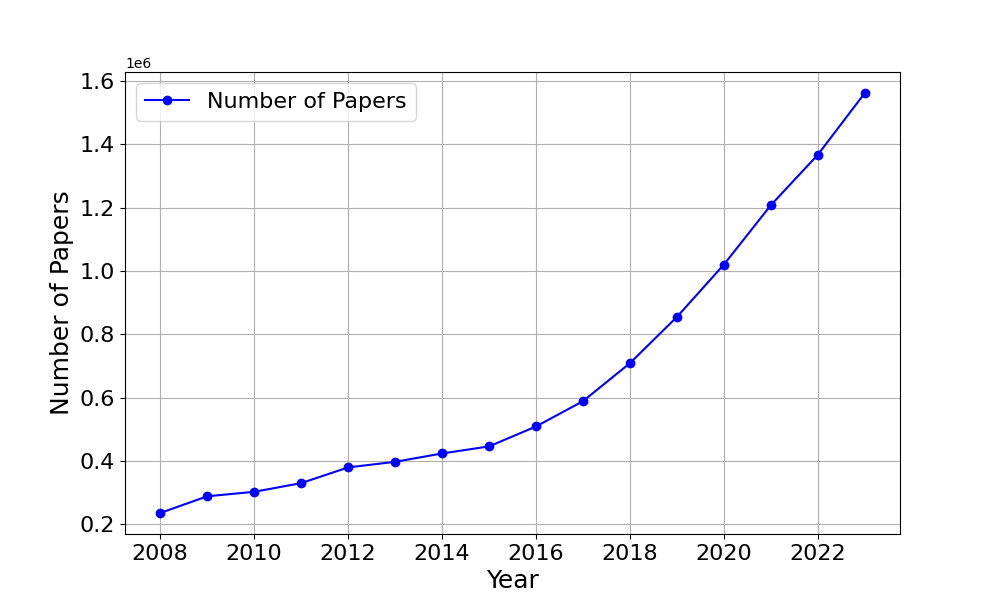
\includegraphics[width=0.75\textwidth]{pub.png}
  \caption{Number of published papers on DNN safety \alex{Increase fonts.}}
  \label{fig:publish}
\end{figure}

An important requirement for DNNs is that they are robust against input perturbations \cite{HuangX}. 
DNNs have shown a lack of robustness due to their vulnerability to adversarial examples, where even minor modifications to an input, sometimes imperceptible to humans, can destabilise the neural network \cite{Goodfellow,Carlini}. Unlike traditional software, DNNs do not have a clear control-flow structure. They learn their decision policy through training on large datasets, adjusting parameters gradually using various methods to achieve the desired accuracy. Figure \ref{fig:Comparison} illustrates the flow of traditional software compared to a neural network. Consequently, traditional software testing methods like functional coverage and branch coverage  cannot be applied to DNNs, thus challenging their use in safety-critical applications. This is because DNNs lack explicit paths and branches that can be directly tested; their behavior emerges from complex interactions within their learned parameters, making it difficult to apply traditional coverage metrics that rely on predefined control flows \cite{Sekhon}.

\begin{figure}
  \centering
  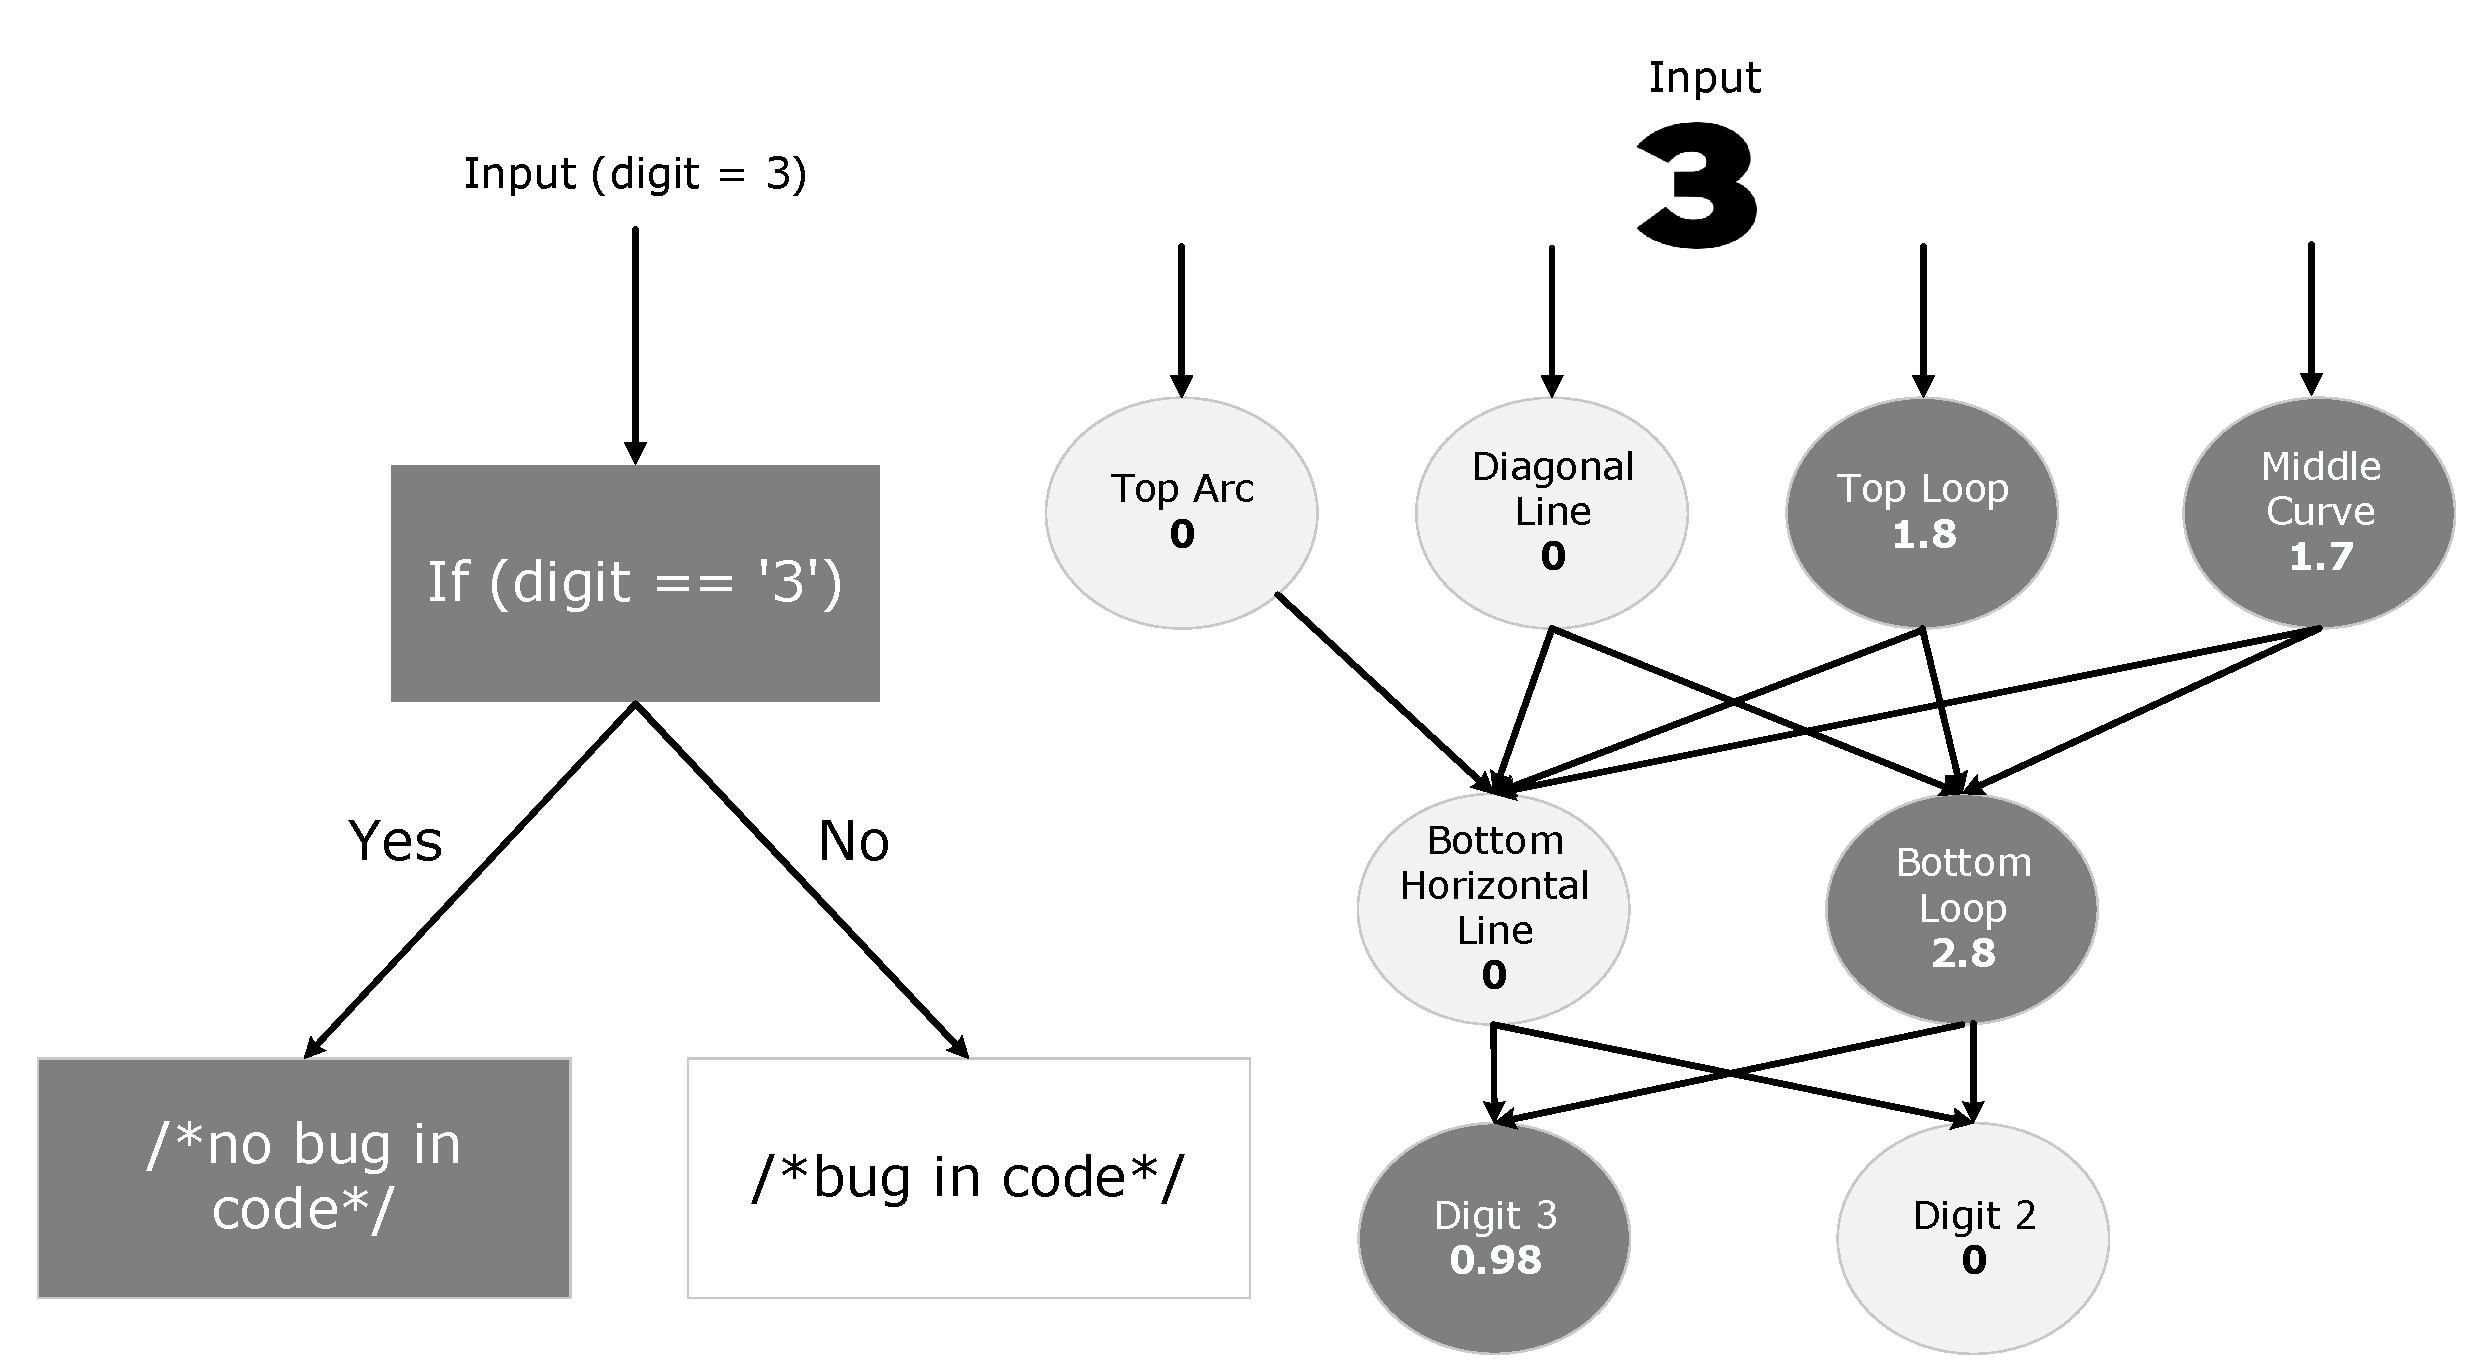
\includegraphics[width=0.75\textwidth]{traditionalandDNN.pdf}
  \caption{Comparison between program flows of a traditional program (left) and a neural network (right). The nodes in gray denote the corresponding basic blocks or neurons that participated while processing an input.}
  \label{fig:Comparison}
\end{figure}

\alex{Missing references} In the past, researchers have extensively discussed both verification and testing techniques, which are useful for evaluating the DNNs. 
\textcolor{purple}{ Verification involves using mathematical proofs to confirm that a model satisfies a specific property, which can refer to characteristics or attributes of the input data or system behavior, such as safety, security, or robustness.}  
% Verification involves proving 
% \alexcomment{the}{a} 
\alexcomment{}{unclear what you say here; parenthesis within a parenthesis}
%  of a \alexcomment{system}{model} \alexcomment{}{Repetition} 
However, DNN verification techniques are promising, they suffer from a scalability problem, due to the high computational complexity and the large size of DNNs. Up to now, DNN verification techniques either work with small scale DNNs or with approximate methods with convergence guarantees on the bounds \cite{HuangX}. This limitation impacts the ability to achieve high coverage, which means to cover all input scenarios and conditions to ensure that all potential issues are identified.

On the other hand, \alexcomment{testing focuses on identifying defects (i.e., counterexample to a property) or provide assurance cases \cite{Rushby}}{To discuss; cannot see the difference between the two} by evaluating the behavior of system through empirical methods. As a result, they can achieve high coverage, which suggests that more of a DNN's behaviour has been tested and therefore the DNN has a lower chance of containing undetected bugs \cite{HuangX}. While these coverage metrics are useful, they often fall short in providing \hyperref[gloss]{\text{comprehensive}}\label{comprehensive} evaluations. This is because they primarily focus on the internal structure of the deep models, such as neuron activation patterns, rather than evaluating the DNNs behaviour on a diverse set of inputs. This internal focus can miss identifying specific inputs that cause failures or unexpected behaviour.


\begin{tcolorbox}[colback=purple!2!white, colframe=purple,title= 10\textsuperscript{th} Month Report Goal]

    The primary aim of my work in the first year is to review existing testing methods for assessing the robustness of DNNs, identify opportunities for improvement, and highlight the need for a fast, scalable, and generalisable end-to-end testing method. This report also aims to outline key research questions and objectives based on these findings and present initial contributions to the field.

\end{tcolorbox}

% \textcolor{olive}{ \textbf{Solution:} To address these limitations, I propose a complete framework that encompasses the entire process from specification to error summarization. This framework will introduce new coverage criteria driven by specific requirements and based on both local and global correctness. Local correctness involves evaluating the AI subsystem's performance on individual inputs representing specific classes, subjected to various transformations, ensuring that the model remains robust under specific conditions. Global correctness assesses the overall behavior of the AI system across a comprehensive range of scenarios, ensuring holistic robustness and reliability. By focusing on testing with specification-driven criteria, my approach aims to provide immediate feedback and uncover a wide range of issues, enhancing the robustness of DNNs.}


\section{\textsc{TestifAI} Overview}

The primary goal of my research is to enhance the robustness of DNNs used in safety-critical systems by designing and implementing a comprehensive testing framework, \textsc{TestifAI}. This framework will formalize specifications related to model architecture, environmental properties and input data characteristics, including the type of data (e.g., images, text), size (e.g., number of samples), size for each class, and the number of classes involved.

\alex{Missing references} The framework will adapt these specifications based on the \textbf{type of testing} being conducted. In \textbf{white-box testing}, full access to the model's internal details (e.g., number of neurons, layers, weights, and types of architectures like CNN, ResNet) is utilized to create precise adversarial examples using methods like FGSM. In \textbf{grey-box testing}, partial access allows the use of input-output pairs and basic model structures (e.g., general architecture without detailed parameters) to train surrogate models that approximate the target model's behavior, enabling the generation of effective test cases without need full internal details. In \textbf{black-box testing}, the framework relies on input-output behavior and environmental properties (e.g., expected input ranges, conditions like rain, dust, brightness, and noise) to iteratively probe and test the model's robustness without internal access. Defining these properties is crucial as it specifies the expected conditions the model should handle.

User requirements, such as specific modules to test and critical scenarios, as well as evaluation metrics (e.g., accuracy, precision, recall), will also be incorporated. If no specific requirements are provided, default parameters will ensure thorough assessment.However, it can also be customized for specific cases or multiple cases based on user specifications. For instance, a user might require the framework to focus on a particular class or scenario that is critical. This flexible and detailed approach aims to provide a robust method for testing DNNs in safety-critical environments.


\alexcomment{To accurately identify weaknesses and areas for improvement, the framework will calculate both local coverage and global coverage using probabilistic programming language that allows you to define bayesian probability models and solve them automatically.}{You introduce new things here that you need to explain in very simple terms: local and global coverage, probabilistic model} This approach allows for a detailed analysis of the model's behavior under different conditions, providing insights into how the model performs in specific scenarios and overall. By examining local-level coverage, the framework can detect vulnerabilities that may arise in specific parts of the model or under particular conditions. Global-level coverage assessment, on the other hand, evaluates the model's overall stability across a wide range of scenarios. Together, these analyses help pinpoint specific vulnerabilities and highlight areas where the model can be improved, ultimately leading to more robust systems.

Additionally, the framework will generate a comprehensive error summary, providing insights into the types and frequencies of errors encountered. This summary will highlight critical failure points and suggest targeted improvements, enabling developers to enhance the system robustness.
Through continuous evaluation and iterative refinement, the framework aims to significantly enhance the safety and dependability of DNN models across different operational levels. This ongoing process ensures that the models remain robust and effective in a wide variety of real-world applications, ultimately contributing to their reliability in safety-critical systems.

\begin{tcolorbox}[colback=purple!2!white, colframe=purple,title= Thesis Goal]
   An end-to-end automated framework that thoroughly integrates data, test cases, and test coverage according to given specifications and provides a detailed error summary.
\end{tcolorbox}

\section{Research Questions and Objectives}
\label{Research Questions and Objectives}
This section outlines the research questions and corresponding objectives of my work:

\begin{enumerate}

    \item \textbf{How can we design a comprehensive framework to test system robustness?} Create a framework that test the DNN under a variety of conditions, ensuring it meets performance standards even in edge cases and adverse scenarios.

  
    \item \textbf{How can we clearly define and specify the properties of the system?} Formalize specifications by developing templates and a specification language that enable users to clearly define and specify the properties of the system and its associated data for testing purposes.

    
    \item \textbf{How can we sample inputs efficiently?} Develop a sampling approach that effectively identifies and prioritizes corner cases. It can be used to guide best selection of inputs for test case generation.
    
    \item \textbf{Can interpretability analysis aid in effective test case generation?} Implement interpretability analysis to identify and prioritize key influential features in the DNN testing process, exploring the use of high influential features for effective test case generation.
   
    \item \textbf{How can we generate highly effective test cases that ensure complete coverage?} Generate highly effective test cases by first developing a sampling approach to collect efficient samples, and then using these samples to identify critical pixels. The identified critical pixels will form the basis for creating test cases that ensure complete coverage and thoroughly assess model vulnerabilities.
 
    \item \textbf{How can we ensure comprehensive test coverage for deep learning models?} Integrate advanced probabilistic methods to evaluate both \hyperref[gloss]{\text{\text{local coverage}}} \label{Local coverage} and \hyperref[gloss]{\text{\text{global coverage}}} \label{Global coverage}.
               
    \item \textbf{How can error summarization be employed to quantify the impacts on model robustness?} Develop method for error summarization that analyze the results of DNNs testing to identify weaknesses. This method will help quantify the impacts of errors on model robustness and provide insights into areas requiring improvement.

\end{enumerate}

\section{Contribution of this Report}

\alex{Missing references}

This report makes the following key contributions: %  to the field of deep learning correctness evaluation:

\begin{itemize}
    \item An \textit{\textcolor{blue}{end-to-end pipeline}} is designed for evaluating the robustness of the system.
    \item A \textit{\textcolor{blue}{hybrid sampling}} technique is proposed to identify and prioritise the corner cases.
    \item A \textit{\textcolor{blue}{conceptual framework}} is proposed that quantifies both local and global robustness. This framework uses Problog, a probabilistic logic programming language, to verify system global robustness.
    \item An \textit{\textcolor{blue}{interpretability-driven test case generation}} approach is employed to pinpoint critical input features, which are then used to create test cases with a higher probability of inducing mispredictions, thus effectively evaluating and enhancing model robustness.
    % \item A novel \textit{error summarization} approach is introduced, which helps in better identifying where model makes mistakes, especially in relation to specific classes and property.
    \item All \textit{\textcolor{blue}{experiments}} are conducted using publicly available datasets, including DAWN, CIFAR, and MNIST.
\end{itemize}

\begin{center}
    \fcolorbox{gray}{lightgray}{
    \parbox{0.95\linewidth}{
    \textbf{Note:} The contributions of this report do not include methods for defining system properties and error summarization technique. Additionally, adversarial examples used in the experiments are taken from existing literature.
    }
    }
    \end{center}
\section{Organization of the Thesis}\hypertarget{organization of thesis}{}
The remainder of the thesis is organized as follows: related studies are presented in Chapter \ref{chp:2}. The system model and proposed methodology are demonstrated in Chapter \ref{chp:3}. Chapter \ref{chp:4} describes the simulation results of our proposed schemes. Finally, the the next two year Phd plan is presented in Chapter \ref{chp:9}.


\clearpage

% Adjusting chapter title format for regular (numbered) chapters
\titleformat{\chapter}[display]
  {\normalfont\huge\bfseries\centering}{\chaptertitlename\ \thechapter}{20pt}{\Huge}

% Using similar styling for unnumbered chapters but without "Chapter" prefix
\titleformat{name=\chapter,numberless}
  {\normalfont\huge\bfseries\centering}{}{0pt}{\Huge}

\titlespacing*{\chapter}{0pt}{50pt}{40pt} % Adjust vertical spacing before and after the title

\chapter{Literature Review}
\label{chp:2}

To develop a comprehensive testing framework for DNNs, it is essential to explore various domains that collectively will contribute to this goal. This literature review will cover the concept of DNN and AI systems, and then examine the robustness of DNNs, including a classification of different types of attacks. Subsequently, the literature will be organized into seven research modules: DNN testing framework, specification, sampling, interpretability, testcase generation, coverage criteria, and error summarization. These modules are not stages of the framework but different areas of research to be explored. Each module will be examined to understand current methods and identifies gaps to develop a comprehensive testing solution.

\section{Deep Neural Networks and AI Systems}

DNNs mimic the structure of the human brain, consisting of millions of interconnected neurons. They extract high-level features from raw input using labeled training data without human interference.

Formally, a DNN is a function $f\colon\mathbb{R}^{s_0}\mapsto \mathbb{R}^{s_k}$ that takes as input a vector of size $s_0$ and produces a vector of size $s_k$. The function $f$ is computed by composing $k$ layers $L_1\colon\mathbb{R}^{s_0} \mapsto\mathbb{R}^{s_1}, \dots, L_k\colon\mathbb{R}^{s_{k-1}}\mapsto\mathbb{R}^{s_k}$ as $f(x) = L_k(\cdots L_2(L_1(x))\cdots)$.

Each layer~$L_i$ typically implements a non-linear function. For instance, a \emph{fully-connected} layer linearly transforms its input $x_{i-1}$ as $W x_{i-1} + b$, where $W\in\mathbb{R}^{s_{i} \times s_{i-1}}$ is the matrix of weights and $b\in\mathbb{R}^{s_i}$ is the bias vector. Then, it applies a non-linear activation function (e.g., sigmoid or rectified linear unit (ReLU)) component-wise, generating the output vector $x_i$. The weights specify how its input neurons are connected to its output neurons and are known as \emph{DNN parameters}. For more information about DNNs, we refer the reader to \cite{dnn_archi, Hassija, Liang}.

The objective of DNN training is to learn parameters during training to make accurate predictions on unseen data during real-world deployment.

When the prediction task is classification, then $s_k$ represents the number of classes. Assuming that $f(x) = (y_1,\dots,y_{s_k})$, the \emph{classification result} is $\displaystyle\mathop{\text{argmax}}_{i=1}^{s_k} y_i$, which is the index of the component with the highest probability $y_i$. By abuse of notation, sometimes we write $f(x)=c$ to denote the fact that $x$ was classified as $c$. We also write $f(x)_c$ to refer to $y_c$ which represents the probability of $x$ being in class $c$.

By an \emph{AI system}, we refer to any software system capable of performing complex tasks through the use of data, algorithms, and high computational power, which typically require human intelligence. These tasks include problem-solving, reasoning, decision-making, and natural language understanding \cite{Illinois}.

Deep learning, a part of AI, uses deep neural networks (DNNs) to recognize complex patterns. Some AI systems are solely based on DNN components, whereas \emph{hybrid} AI systems combine DNNs with traditional software to produce the final output.

\section{Robustness of Deep Neural Networks}

\begin{figure*}[h]
  \centering
  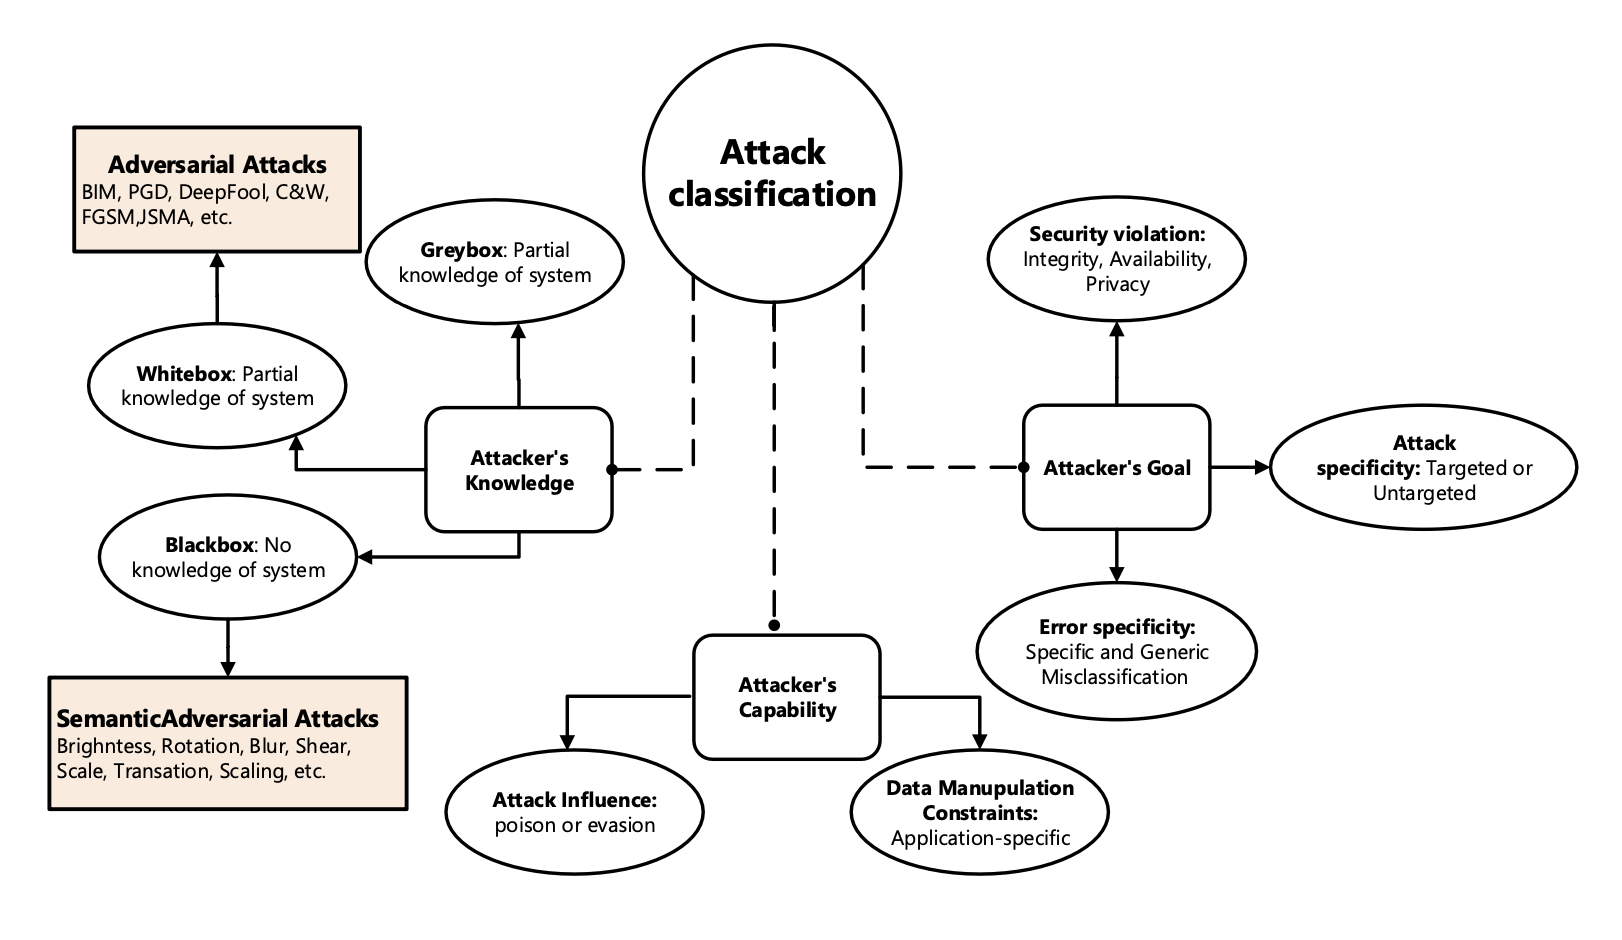
\includegraphics[width=\linewidth]{attackclassification.png}
  \caption{Attack classification}
  \label{fig:adv_threats}
\end{figure*}


DNNs are known for their lack of robustness, which makes them vulnerable to adversarial attacks. Researchers have developed various attack techniques to expose these vulnerabilities by creating adversarial examples, which highlight the weaknesses of a DNN without providing any provable guarentee \cite{HuangX}. Fig. \ref{fig:adv_threats}  illustrates the different types of attack threats, emphasizing the complexity and variety of these attacks. Adversarial attacks can be categorized through three main components: attacker's knowledge, attacker's goals, and attacker's capabilities \cite{Biggio}.

Attackers can have different levels of knowledge about DNN: white-box attacks have full knowledge of the architecture and parameters, gray-box attacks have partial knowledge, and black-box attacks have no knowledge and rely on input-output queries. Their goals might include compromising system integrity, availability, or privacy. Attack specificity can be targeted, aiming to misclassify a specific set of samples, or untargeted, causing any sample to be misclassified. 
Error specificity refers to whether the attacker aims for misclassification as a specific class or any incorrect class. Attackers can influence the model by poison attack \cite{poisonattack,Badnets} during training or evasion attack \cite{evasion} during testing, and these manipulations are often constrained by application-specific data alteration limits.\cite{Chakraborty}.

In the context of attacker's knowledge, different techniques are proposed in literature to create \emph{adversarial examples}. White-box attacks, such as the Fast Gradient Sign Method (FGSM) \cite{FGSM}, Basic Iterative Method (BIM) \cite{BIM}, Carlini and Wagner (C\&W) Attack \cite{Carlini}, DeepFool \cite{deepfool}, and Jacobian-based Saliency Map Attack (JSMA) \cite{JSMA}, use different internal information of the DNN. These techniques use gradients (FGSM, BIM, C\&W), decision boundaries (DeepFool), and the Jacobian matrix of the output with respect to the input (JSMA) to generate effective adversarial examples. They specifically manipulate input data to create slight perturbations that maximize the network prediction error, causing the DNN to make incorrect predictions \cite{Hosseini}.

Conversely, black-box attacks do not rely on internal information of the DNN to craft adversarial examples. These attacks often involve \emph{semantic adversarial examples} \cite{HuangX,deeptest,Engstrom,Pei}, which are not limited to slight modifications of the image. These attacks can involve any transformation that preserves the semantics of the image, such as shear, translation, scale, rotations, etc., as illustrated in Fig. \ref{fig:image-trans}.


\begin{center}
  \fcolorbox{gray}{lightgray}{
  \parbox{0.95\linewidth}{
  \textbf{Note:} Currently, I have explored both black-box and white-box techniques to understand the differences between these adversarial examples. Further exploration is needed for grey-box techniques.

  }
  }
  \end{center}

  \begin{figure*}
    \centering
    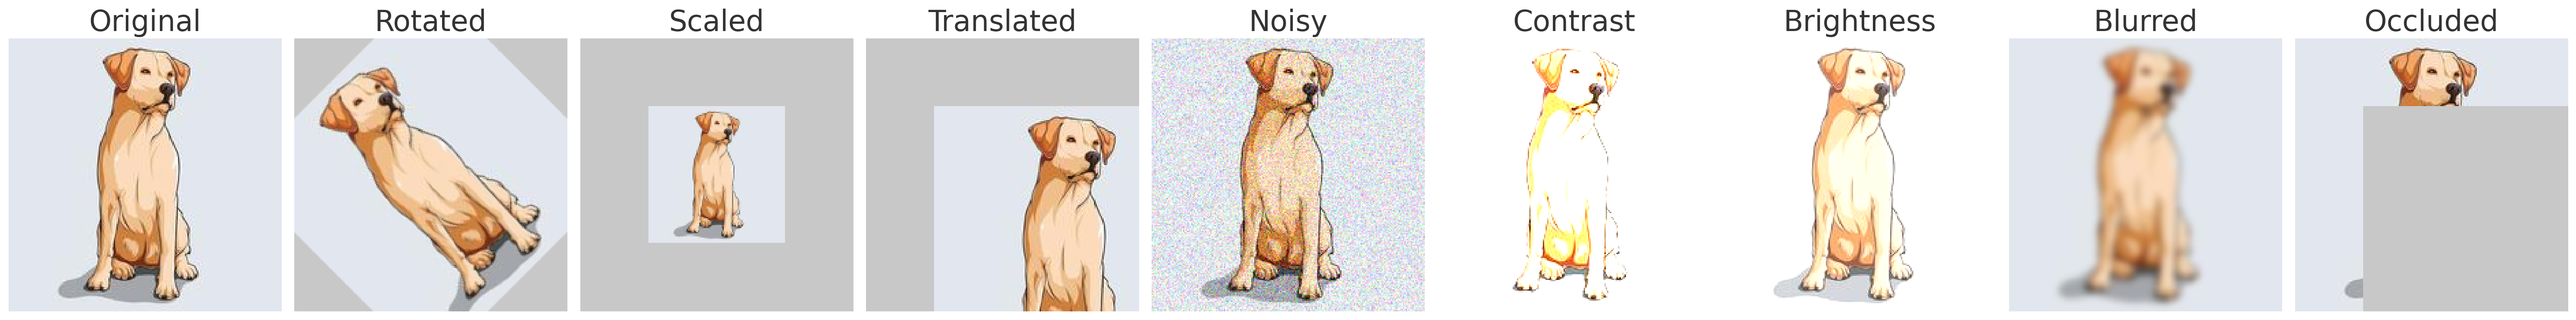
\includegraphics[width=\linewidth]{figures/output_update.png}
    \caption{Semantic Adversarial Examples}
    \label{fig:image-trans}
  \end{figure*}


\section{Research Modules}

I have categorized the literature work into seven research areas as shown in Figure \ref{fig:thematic_wheel}. 
\begin{figure*}[h]
  \centering
  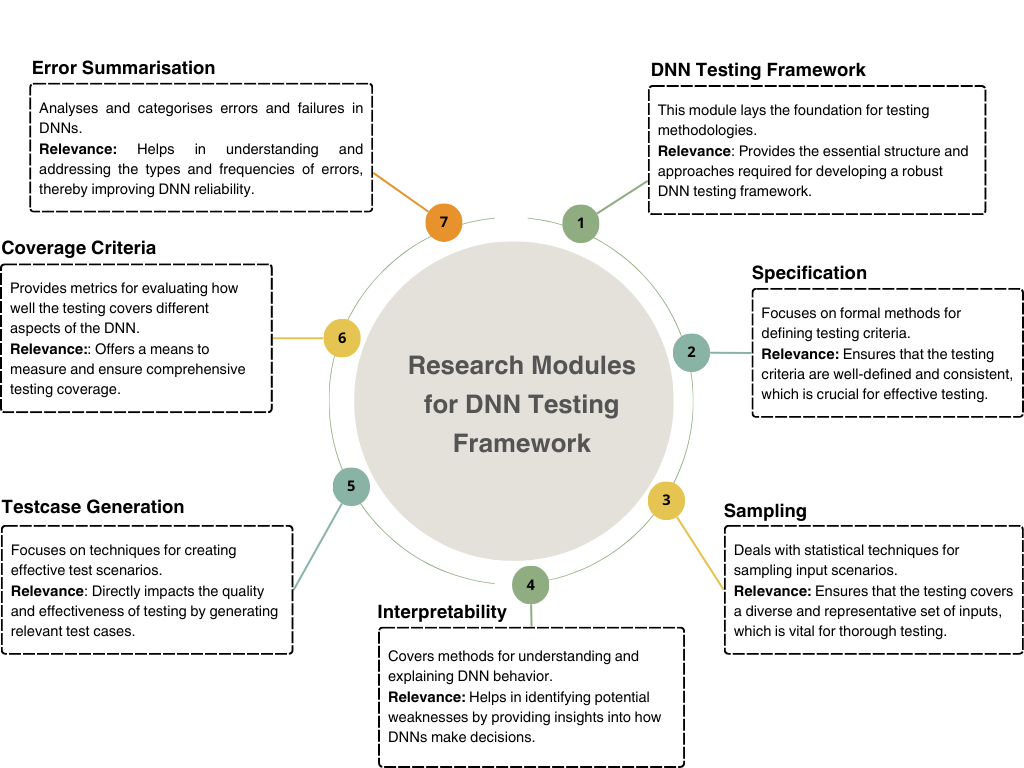
\includegraphics[width=\linewidth]{literaturedomains.png}
  \caption{Thematic Wheel Diagram of Research Modules for DNN Testing Framework}
  \label{fig:thematic_wheel}
\end{figure*}

Various frameworks have been proposed in the literature, each incorporating different methodologies and components to address specific aspects of DNN testing and related research areas. Braiek and Khomh in paper \cite{Braiek} reviews all the challenges of testing DNNs, discussing each area but without providing concrete solutions. Table \ref{tab:Comprison of Research Modules} provides a comparison of several papers based on their inclusion of key areas such as specification, sampling, interpretability, testcase generation, coverage criteria, and error summarization.
 It indicates that no single paper comprehensively addresses all the areas necessary for a robust DNN testing framework.  Most research, such as \cite{Sekhon},  \cite{deeptest},\cite{deepxplore},\cite{Wicker}, \cite{Ma}, \cite{SunY}, \cite{Sun}, \cite{Cheng}, \cite{Kim}, \cite{Concolic}, \cite{Deepconcolic}, \cite{tensorfuzz}, \cite{Deephunter}, \cite{DLFuzz}, \cite{Sayah}, and \cite{Dola}, focuses on testcase generation and coverage criteria, providing methods to generate effective test cases and evaluate DNNs. 


 Expanding on this foundational work, test-case generation methods are influenced by traditional software testing methods like fuzz testing, metamorphic testing, and symbolic execution. DeepXplore \cite{deepxplore} is a whitebox test-case generation method that checks how different DNNs behave using domain-specific rules on inputs. It uses multiple models trained on the same data to find differences in their prediction. It aims to jointly optimize neuron coverage and different predictions between models, using gradient ascent for test generation. DeepTest \cite{deeptest} focuses on generating test inputs for autonomous cars by applying domain-specific rules on seed inputs. It uses a greedy search method based on the NC metric to create effective test cases. Adapting traditional fuzzing techniques for DNN test-case generation includes methods like DLFuzz \cite{DLFuzz} and TensorFuzz \cite{tensorfuzz}. DLFuzz generates adversarial inputs based on neuron coverage, akin to DeepXplore, but does not require multiple models and uses constraints to keep new inputs similar to originals. TensorFuzz employs coverage-guided testing to uncover numerical issues and discrepancies in DNNs and their quantized versions. DeepConcolic \cite{Deepconcolic} employs a concolic testing approach to generate adversarial inputs for DNN testing. It combines symbolic execution with concrete execution path information to meet coverage criteria, supporting both NC and MC/DC criteria.

In traditional software testing, coverage criteria measure how thoroughly software is tested. In DNNs, coverage might not directly apply to lines of code but rather to the input space or the variety of data the model can effectively handle or provide predictions for. Neuron coverage (NC) \cite{deepxplore} is the first coverage metric proposed in the literature to test DNNs. It is defined as the ratio of neurons activated by a test input to the total number of neurons in the model, where a neuron is activated when its activation value exceeds a predefined threshold. Ma et al. \cite{Ma} proposed a variety of coverage metrics, including K-multisection neuron coverage (KMNC), Neuron boundary coverage (NBC), and Strong neuron activation coverage (SNAC). KMNC calculates coverage by dividing the interval between lower and upper bounds into k-bins and measuring the number of bins activated by the test inputs. NBC measures the ratio of corner case regions covered by test inputs, with corner cases defined as activation values below or above those observed during training. SNAC similarly measures how many upper corner cases, defined as activation values above the training range, are covered by test inputs. Modified Condition/Decision Coverage (MC/DC) \cite{SunY} captures causal changes in test inputs based on the sign and value change of a neuron's activation. Likelihood-based Surprise Adequacy (LSA) uses Kernel Density Estimation (KDE) to estimate the likelihood of a test input during the training phase, prioritizing inputs with higher LSA scores as they are closer to classification boundaries. Distance-based Surprise Adequacy (DSA) is an alternative to LSA that uses the distance between activation traces of new test inputs and those observed during training \cite{Kim}.

Efficient sampling methods, crucial for identifying representative input scenarios, have not been the primary focus of existing studies. Sampling is a crucial step in the testing of DNNs, as it involves selecting a representative subset of inputs from a potentially vast input space. Depending on the testing objectives, different sampling techniques can be employed to ensure comprehensive testing. Stratified sampling ensures that all groups (or strata) within the data are represented, which is particularly useful when the specification requires equal representation from all categories. This technique needs prior knowledge of the groups to be effective \cite{Stratifiedsampling}. When the focus is on identifying critical samples, techniques like Borderline-SMOTE, ADASYN, and NearMiss are particularly useful. Borderline-SMOTE generates synthetic examples near the class borders, targeting challenging areas and thus helping to identify corner cases. However, it can still introduce noise \cite{Han2005}. ADASYN (Adaptive Synthetic Sampling Approach for Imbalanced Learning) adjusts the number of synthetic samples generated for each minority class example according to its difficulty level, focusing more on difficult-to-learn examples but might also introduce noise \cite{He2008}. NearMiss focuses on selecting examples close to the decision boundary, emphasizing difficult examples, but may discard useful information \cite{near-miss}. Integrating advanced sampling techniques into DNN testing and addressing their challenges can enhance corner case identification. Current research primarily focuses on generating effective input test cases through semantic adversarial examples or adversarial examples. However, it is crucial to first understand whether the samples selected for these test cases are optimal. By prioritizing the selection of high-quality samples, we can lay a stronger foundation for subsequent test case generation, leading to more reliable and insightful testing outcomes. This shift in focus could provide new directions for research and development in DNN testing, ensuring that the inputs used for test cases are truly representative and capable of revealing critical vulnerabilities.

Formal specification of testing requirements is another area that lacks attention in current research. Paper \cite{Scenic} introduces Scenic, a language specifically designed for scenario specification and scene generation, highlighting its utility in creating detailed and probabilistic environment models. While some papers on interpretability, such as \cite{Fidel, Lin, Walker, Rahnama, Watson, Kuppa} exist in the literature, they primarily focus on detecting adversarial examples rather than providing a comprehensive framework for DNN testing. Although interpretability is not a key component of my framework, it is an important area of research that I will use for test case generation. Additionally, error summarization is covered by even fewer papers. For instance, \cite{ChenJ} omprehensive analysis of different types of bugs, identifies common bug patterns and their root causes to guide more effective debugging practices. Similarly, the authors of \cite{Deepmutation} analyzed the differences between the original and mutated models to identify errors.

\begin{table*}[ht]
  \centering
  \renewcommand{\arraystretch}{1.5}
  \setlength{\tabcolsep}{8pt}
  \resizebox{\textwidth}{!}{
  \begin{tabular}{|>{\centering\arraybackslash}m{3.5cm}|>{\centering\arraybackslash}m{2.5cm}|>{\centering\arraybackslash}m{2.5cm}|>{\centering\arraybackslash}m{3cm}|>{\centering\arraybackslash}m{3.5cm}|>{\centering\arraybackslash}m{3.5cm}|>{\centering\arraybackslash}m{3.5cm}|}
  \hline
  \rowcolor[gray]{0.9} \textbf{Paper} & \textbf{Specification} & \textbf{Sampling} & \textbf{Interpretability} & \textbf{Testcase Generation} & \textbf{Coverage Criteria} & \textbf{Error Summarization} \\
  \hline
  ImprovedTesting\cite{Sekhon} & \tickNo & \tickNo & \tickNo & \tickYes & \tickYes & \tickNo \\
\hline
  Deeptest \cite{deeptest} & \tickNo & \tickNo & \tickNo & \tickYes & \tickYes & \tickNo \\
  \hline
  DeepXplore \cite{deepxplore} & \tickNo & \tickNo & \tickNo & \tickYes & \tickYes & \tickNo \\
  \hline
  Feature-guided Testing \cite{Wicker}& \tickNo & \tickNo & \tickNo & \tickYes & \tickYes & \tickNo \\
\hline
DeepGauge \cite{Ma}& \tickNo & \tickNo & \tickNo & \tickYes & \tickYes & \tickNo \\
  \hline
  Testing DNNs \cite{SunY}& \tickNo & \tickNo & \tickNo & \tickYes & \tickYes & \tickNo \\
\hline
Structural Test Coverage \cite{Sun}& \tickNo & \tickNo & \tickNo & \tickYes & \tickYes & \tickNo \\
\hline

Quantitative Projection Coverage \cite{Cheng} & \tickNo & \tickNo & \tickNo & \tickYes & \tickYes & \tickNo \\
\hline
Surprise Adequacy \cite{Kim} & \tickNo & \tickNo & \tickNo & \tickYes & \tickYes & \tickNo \\
\hline
Concolic testing \cite{Concolic} & \tickNo & \tickNo & \tickNo & \tickYes & \tickYes & \tickNo \\
\hline
Deepconcolic \cite{Deepconcolic} & \tickNo & \tickNo & \tickNo & \tickYes & \tickYes & \tickNo \\
\hline
Tensorfuzz \cite{tensorfuzz} & \tickNo & \tickNo & \tickNo & \tickYes & \tickYes & \tickNo \\
\hline
Deephunter \cite{Deephunter} & \tickNo & \tickNo & \tickNo & \tickYes & \tickYes & \tickNo \\
\hline
DLFuzz \cite{DLFuzz} & \tickNo & \tickNo & \tickNo & \tickYes & \tickYes & \tickNo \\
\hline
Symbolic execution\cite{Gopinath} & \tickNo & \tickNo & \tickNo & \tickYes & \tickNo & \tickNo \\
\hline
Automated Test Generation\cite{Agarwal} & \tickNo & \tickNo & \tickNo & \tickYes & \tickNo & \tickNo \\
\hline
DeepRoad \cite{Zhang} & \tickNo & \tickNo & \tickNo & \tickYes & \tickNo & \tickNo \\
\hline
MODE \cite{MODE} & \tickNo & \tickNo & \tickNo & \tickYes & \tickNo & \tickNo \\
\hline
Deepmutation \cite{Deepmutation} & \tickNo & \tickNo & \tickNo & \tickYes & \tickYes & \tickYes \\
% \hline
% \cite{Braiek} & \tickYes & \tickYes & \tickYes & \tickYes & \tickYes & \tickYes \\
\hline
Distribution-aware testing \cite{Dola} & \tickNo & \tickNo & \tickNo & \tickYes & \tickYes & \tickNo \\
\hline
Robustness testing \cite{Sayah} & \tickNo & \tickNo & \tickNo & \tickYes & \tickYes & \tickNo \\
\hline
Understanding Framework Bugs\cite{ChenJ} & \tickNo & \tickNo & \tickNo & \tickYes & \tickYes & \tickYes \\
\hline
%Specification
Scenic\cite{Scenic} & \tickYes & \tickNo & \tickNo & \tickNo & \tickNo & \tickNo \\
\hline
% SHAP
SHAP signatures\cite{Fidel} & \tickNo & \tickNo & \tickYes & \tickNo & \tickNo & \tickNo \\
\hline
DeepSHAP \cite{Lin} & \tickNo & \tickNo & \tickYes & \tickNo & \tickNo & \tickNo \\
\hline
Attribution Analysis \cite{Walker} & \tickNo & \tickNo & \tickYes & \tickNo & \tickNo & \tickNo \\
\hline
Adversarial Explaining \cite{Rahnama} & \tickNo & \tickNo & \tickYes & \tickNo & \tickNo & \tickNo \\
\hline
Attack-Agnostic Detection\cite{Watson} & \tickNo & \tickNo & \tickYes & \tickNo & \tickNo & \tickNo \\
\hline
XAI\cite{Kuppa} & \tickNo & \tickNo & \tickYes & \tickNo & \tickNo & \tickNo \\
\hline
%sampling
Stratified sampling\cite{Stratifiedsampling} & \tickNo & \tickYes & \tickNo & \tickNo & \tickNo & \tickNo \\
\hline
Borderline-SMOTE \cite{Han2005} & \tickNo & \tickYes & \tickNo & \tickNo & \tickNo & \tickNo \\
\hline
ADASYN\cite{He2008} & \tickNo & \tickYes & \tickNo & \tickNo & \tickNo & \tickNo \\
\hline
Near-Miss\cite{near-miss} & \tickNo & \tickYes & \tickNo & \tickNo & \tickNo & \tickNo \\
\hline
  \end{tabular}
  }
  \caption{Comparison of Research Areas Relevant to DNN Testing}
  \label{tab:Comprison of Research Modules}
  \end{table*}



% [Comment for Alex]  I will revisit and complete this PLP section at the end of the document. Currently, I am unable to integrate it smoothly into the flow of the literature review.


% \section{Probabilistic Logic Programming (PLP)}

% Probabilistic Logic Programming (PLP) integrates probabilistic reasoning with the flexibility and expressiveness of logic programming. Traditional logic programming paradigms are deterministic, where each statement is either true or false. However, real-world scenarios often involve inherent uncertainties which deterministic logic cannot adequately handle. PLP addresses this limitation by allowing the representation of uncertainties directly within the logic framework, thereby enabling more nuanced and accurate modeling of complex domains \cite{Sato2001, Kimmig2011}.

% PLP has been explored extensively in various domains, including artificial intelligence, bioinformatics, and robotics. Sato and Kameya's introduction of PRISM \cite{Sato1997} was a significant milestone, combining statistical modeling with logic programming. Subsequent work by Koller and Friedman \cite{Koller2009} on probabilistic graphical models further influenced PLP frameworks. Various approaches to PLP, such as Logic Programs with Annotated Disjunctions (LPADs) \cite{Vennekens2004}, ProbLog \cite{DeRaedt2007}, Probabilistic Horn Abduction (PHA) \cite{Poole1993}, Independent Choice Logic (ICL) \cite{Poole1997}, and PRISM \cite{Sato2001}, have been developed, each leveraging the distribution semantics introduced by Sato \cite{Sato2001}.

% Among these, ProbLog has gained prominence due to its simplicity and expressive power, making it a preferred choice for many applications \cite{Kimmig2011}. ProbLog extends a logic program with probabilistic facts, defining a probability distribution over possible worlds (sets of facts). The probability of a query is computed by marginalizing over the probabilities of the worlds where the query is true.

% The need for explainable AI (XAI) has become increasingly important, particularly in domains where decisions must be transparent and interpretable, such as medical diagnosis and finance. Various approaches to XAI emphasize model interpretability and the generation of comprehensible explanations for model predictions \cite{Arrieta2020}. PLP, with its ability to generate explanations as part of its reasoning process, fits well within the XAI paradigm. Vidal \cite{Vidal2023} proposes a novel approach where explanations in PLP are represented as programs generated from a given query through unfolding-like transformations. This approach preserves the causal structure of inferences and ensures minimality by excluding irrelevant information. Such explanations can be parameterized to hide uninteresting details, making them comprehensible to non-expert users.


% Despite the extensive research in PLP and its applications, its use in testing DNNs is still very new. DNNs are powerful but often act like "black boxes," making it hard to understand and trust their predictions. This thesis presents a new way to use PLP for testing DNNs, an area that has not been explored before.

% By using PLP, we can turn the probabilistic outputs  of DNNs into probabilistic facts and rules. This helps in reasoning about uncertainties in the model's predictions and generating clear explanations for each prediction. This approach makes it easier to understand why a model made a certain prediction, giving insights into the model’s decision-making process. PLP can also help in debugging DNNs by identifying and fixing inconsistencies or unexpected behaviors in the predictions. By examining the probabilistic rules and their explanations, we can find areas for improvement more effectively. Additionally, PLP allows us to simulate different scenarios by changing probabilistic facts, which is useful for testing how robust the DNNs are under various conditions. This innovative method opens up new opportunities for research and practical applications, making deep learning systems more transparent, reliable, and trustworthy.


% Adjusting chapter title format for regular (numbered) chapters
\titleformat{\chapter}[display]
  {\normalfont\huge\bfseries\centering}{\chaptertitlename\ \thechapter}{20pt}{\Huge}

% Using similar styling for unnumbered chapters but without "Chapter" prefix
\titleformat{name=\chapter,numberless}
  {\normalfont\huge\bfseries\centering}{}{0pt}{\Huge}

\titlespacing*{\chapter}{0pt}{50pt}{40pt} % Adjust vertical spacing before and after the title

\chapter{Proposed Framework} % Ensures chapter numbering starts correctly
\label{chp:3}


This chapter presents a comprehensive approach for AI systems, which may consist of one or multiple DNN components, each component handle different task. My research introduces a framework that addresses each DNN separately, recognising that each has unique specifications, e.g., consider an AI system using the MNIST dataset for different purposes. One DNN might classify handwritten digits (0-9), while another might analyse pairs of digits to predict their sum or product. Although both DNNs work with digit images in this case, their properties in specifications differ due to their distinct tasks, even when using the same dataset. In other cases, such as an autonomous car, different DNNs might use different datasets designed for their specific tasks. One DNN might use labeled images for object detection (e.g., identifying pedestrians, vehicles, and road signs), while another DNN might use data on driving paths and movement for path planning to predict optimal routes. This framework provides end-to-end testing for each DNN. It consists of five components, summarized in Figure~\ref{fig:framework}.

\begin{enumerate}
  \item \emph{Specification} defines key properties to guide testing. It includes details about the DNN architecture, environmental properties, and input data, like data type, sample size, and number of classes. 
    \item \emph{Sampling} involves selecting a representative subset of inputs from a potentially vast input space. Depending on the testing objectives, this subset helps ensure that the tests are meaningful and cover various scenarios effectively.
    \item \emph{Testcase Generation} applies the properties mentioned in the specifications to the sampled data to generate test cases.
    \item \emph{Testing Graph Analysis} conducts both local and global coverage assessments. Locally, it focuses on an individual property to check its correctness. Globally, it examines multiple properties to understand their interdependencies and overall system behavior. By modeling these dependencies probabilistically, testing graph analysis provides a comprehensive view of AI system.
    \item \emph{Error Summarisation} quantify the performance of the AI system by compiling and analyzing recorded errors. This analysis generates graphical reports and recommendations, helping to refine and improve the models.
\end{enumerate}

\begin{figure*}
  \centering
  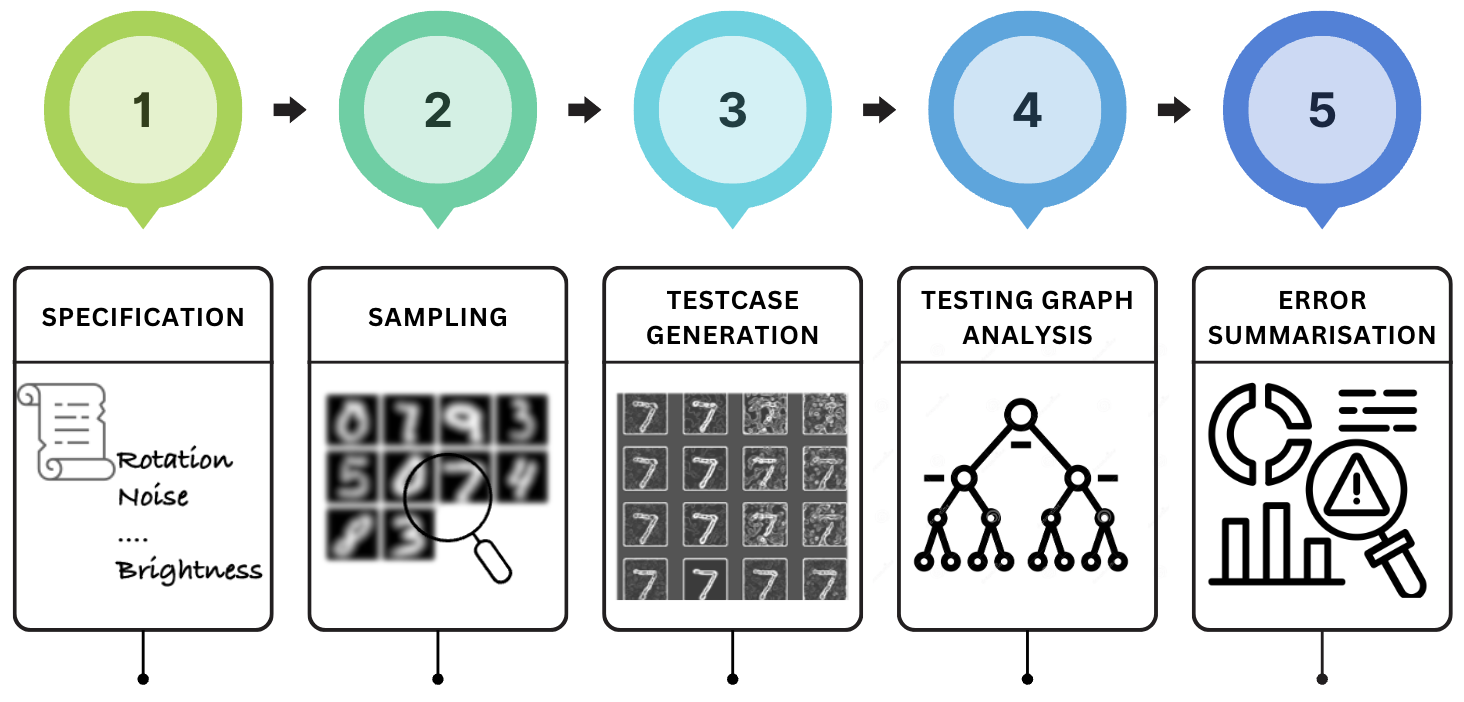
\includegraphics[width=\linewidth]{figures/fivesteps.png}
  \caption{Overview of the Proposed Framework}
  \label{fig:framework}
\end{figure*}

My research focus on AI systems with DNN components performing various tasks, which may include classification, regression, clustering and more. Each DNN within the system has unique specifications. Formally, we define an AI system $ \mathcal{S} $ as follows:

$\mathcal{F}$ is the functional unit comprises $n$ DNN components $ f_1, \dots, f_n $, each handling different tasks, and a symbolic (software) component $ \omega $ that integrates the outputs of these DNNs. Given an input $\vec{x} = (x_1, \dots, x_n)$, where each $x_i$ represents an input from the respective dataset of $f_i$, the output $\mathcal{F}(\vec{x})$ is defined as $\omega(f_1(x_1), \dots, f_n(x_n))$. Each DNN component $f_i$ processes its input $x_i$ according to its specific dataset.


\section{Specification}
The first component of this framework is formalized to specify model architecture $\mathcal{M}$, environmental properties, testing type, and input data characteristics $\mathcal{D}$. 

The specifications $\mathcal{S}_{\text{specs}}$ include all classes (classification task) by default, but users can adjust this to test specific classes based on their needs.

It is essential to specify the type of testing $\mathcal{T}$ within the $\mathcal{S}_{\text{specs}}$, as different methods are employed based on this choice. In black-box testing $\mathcal{T}_{\text{black}}$, semantic adversarial properties $\mathcal{P}_{\text{sem}}$ are applied by adjusting the input data $\mathcal{D}$ without any knowledge of the model's internal details. In white-box testing $\mathcal{T}_{\text{white}}$, adversarial attacks $\mathcal{P}_{\text{adv}}$ are used by accessing the model's internal structure and parameters. Grey-box testing $\mathcal{T}_{\text{grey}}$ combines aspects of both, utilizing partial knowledge of the model’s structure to inform the testing process. 



\begin{example}
  \label{ex:mnist-adder-specification}
  Consider the AI system $\mathcal{S}_{\text{adder}}$, an \emph{MNIST Digit Adder}, which is specified as $\mathcal{S}_{\text{adder}} = (\mathcal{F}, \mathcal{D})$. In this system, the functional unit $\mathcal{F}$ consists of a DNN component $\mathcal{M}_{\text{CNN}}$, which is a Convolutional Neural Network (CNN) designed to recognize digits ranging from 0 to 9. The dataset $\mathcal{D}$ provides input in the form of images, and a software component $\omega$ is used to perform the addition of the recognized digits. 

  Formally, we define $\mathcal{F} = (\{\mathcal{M}_{\text{CNN}}\}, \omega)$, where $\omega$ integrates the output of the DNN. The function $\mathcal{M}_{\text{CNN}}$ takes single digit as an input and recognizes the digits. The software component $\omega$ can then pick any two recognized digits and compute their sum. For example, $\mathcal{S}_{\text{adder}}$ can perform the task of digit addition:
  \begin{equation}
    \mathcal{S}_{\text{adder}}(x_1, x_2) = \omega(\mathcal{M}_{\text{CNN}}(x_1), \mathcal{M}_{\text{CNN}}(x_2)),
  \end{equation}
  where $\omega(a, b) = a + b$. Given two digits $x_1$ and $x_2$, $\mathcal{S}_{\text{adder}}$ recognizes the digits and computes their sum.

  The specifications $\mathcal{S}_{\text{specs}}$ for this system include the following key elements: The DNN component $\mathcal{M}_{\text{CNN}}$ is a pre-trained CNN with a typical architecture involving a convolutional layer (32 filters, kernel size 3x3, ReLU activation), followed by a max pooling layer (2x2), a flattened layer, a fully connected layer with 128 neurons (ReLU), and an output layer with 10 neurons using softmax activation. The input data $\mathcal{D}$ consists of 10,000 test samples of digits, each labeled with one of 10 classes representing the digits 0 to 9. 

  $\mathcal{S}_{\text{adder}}$ is evaluated using both black-box and white-box testing methods. In black-box testing $\mathcal{T}_{\text{black}}$, semantic adversarial properties such as rotation, brightness adjustment, blur, shear, and contrast modification are applied to the input data without accessing the internal structure of $\mathcal{M}_{\text{CNN}}$. Specifically, $\mathcal{S}_{\text{adder}}$ robustness is tested against rotations within a range of 3 to 30 degrees and brightness adjustments between 0.5 and 1.5. In white-box testing $\mathcal{T}_{\text{white}}$, adversarial examples are generated by utilizing the internal structure and parameters of $\mathcal{M}_{\text{CNN}}$, like Fast Gradient Sign Method (FGSM), Projected Gradient Descent (PGD), AdamPGD, and Deepfool.
\end{example}


\textbf{Note:} Grey-box testing, involving partial model access, will be explored in future work.
\section{Sampling}
The sampling process is designed to identify both efficient and corner cases, focusing on hard-to-learn examples to enhance the robustness of the model. Data is sampled according to the requirements specified in the specifications. By default, all classes are tested, but users can customize the classes to be sampled based on specific requirements. The sampling approach is applied as follows for each classifier $f_i$ independently:

The full sample $\mathcal{X}_i$ for classifier $f_i$, $i=1,\dots,n$, is computed by applying the sampling method directly to the dataset $\mathcal{D}_i$:

\begin{equation}
\mathcal{X}_i = \text{Sampling}(\mathcal{D}_i)
\end{equation}

Here, $\mathcal{D}_i$ represents the dataset associated with each classifier $f_i$. In cases where all classifiers share the same dataset, $\mathcal{D}_i$ may be identical across all $i$, denoted simply as $\mathcal{D}$. However, if the datasets differ for each classifier, they are represented individually as $\mathcal{D}_1, \mathcal{D}_2, \dots, \mathcal{D}_n$ to reflect the specific dataset for each $f_i$.



This sampling method is designed to balance the dataset and ensure that both typical and challenging cases are adequately represented, thereby improving the evaluation of the model's performance across a variety of scenarios.


\begin{example}
  \label{ex:sampling}
  To further illustrate the sampling process, consider the classifier $\mathcal{M}_{\text{CNN}}$ and $\mathcal{D}$ from Example~\ref{ex:mnist-adder-specification}. For each class $c$ in $\mathcal{D}$, we begin with the samples specified in specification, forming the initial subset $\mathcal{X}_{\text{mnist}}$. This subset is then enhanced by applying a hybrid sampling method, that combines Borderline-SMOTE focuses on creating samples near decision boundaries, while ADASYN targets hard-to-learn examples, ensuring that both typical and challenging cases are effectively covered. The final sample $\mathcal{X}_{\text{hyb}}$ for testing is obtained as:
  

  \begin{equation}
    \mathcal{X}_{\text{hyb}} = \text{HybridSampling}(\mathcal{X}_{\text{mnist}})
  \end{equation}

  where $\mathcal{X}_{\text{hyb}}$ is new sampled data. HybridSampling method combines Borderline-SMOTE and ADASYN. This process ensures a balanced and comprehensive set of test samples, covering both typical and challenging cases for robust evaluation of $\mathcal{M}_{\text{CNN}}$.
\end{example}




\begin{tcolorbox}[colback=purple!2!white, colframe=purple, title=Challenges in Sampling]
  \begin{itemize}
    \item \textbf{Synthetic Sample Quality:} Ensuring generated samples represent true corner cases, not noise.
    \item \textbf{Computational Overhead:} Managing the intensive computation required for hybrid sampling.
 
  \end{itemize}

\end{tcolorbox}


\section{Test Case Generation}

The test case generation process is designed to create a comprehensive set of test cases that evaluate the robustness of the AI system, as outlined in the specifications. Test cases are generated by applying specified perturbations to the resampled data, ensuring that the system is rigorously evaluated under various conditions.

For each classifier $f_i$, $i = 1, \dots, n$, test cases are generated based on the perturbations defined in the specifications. The test cases $\mathcal{T}_i$ for classifier $f_i$ are generated as follows:

\begin{equation}
\mathcal{T}_i = \text{GenerateTestCases}(\mathcal{X}_i, \mathcal{P}_i)
\end{equation}

Here, $\mathcal{X}_i$ represents the sampled data for classifier $f_i$, and $\mathcal{P}_i$ denotes the set of perturbations to be applied. The method $\text{GenerateTestCases}$ applies these perturbations to create the test cases, which are then used to assess the model's performance.

\begin{example}
  \label{ex:test-case-generation-math}
   $\mathcal{S}_{\text{adder}}$ evaluated using both black-box and white-box testing methods as specified in Example~\ref{ex:mnist-adder-specification}. The test cases are generated by applying various perturbations to the resampled data $\mathcal{X}_{\text{hyb}}$ for classifier $\mathcal{M}_{\text{CNN}}$ mentioned in Example~\ref{ex:mnist-adder-specification}.

  For black-box testing, let $\mathcal{P}_{\text{black}} = \{\text{Rotation}, \text{Brightness}, \text{Blur}, \text{Shear}, \text{Contrast}\}$ represent the set of semantic adversarial properties applied without accessing the internal structure of $\mathcal{M}_{\text{CNN}}$. The test cases generated for black-box testing are:
  
  \begin{equation}
  \mathcal{T}_{\text{black},i} = \bigcup_{p \in \mathcal{P}_{\text{black}}} \text{ApplyPerturbation}(p, \mathcal{X}_{\text{hyb}})
  \end{equation}
  
  For white-box testing, where the internal structure of $\mathcal{M}_{\text{CNN}}$ is utilized, let $\mathcal{P}_{\text{white}} = \{\text{FGSM}, \text{PGD}, \text{AdamPGD}, \text{Deepfool}\}$ represent the set of adversarial attack methods. The test cases generated for white-box testing are:
  \begin{equation}
  \mathcal{T}_{\text{white},i} = \bigcup_{a \in \mathcal{P}_{\text{white}}} \text{GenerateAdversarial}(a,\mathcal{X}_{\text{hyb}}, \mathcal{M}_{\text{CNN}})
  \end{equation}

  The overall set of test cases $\mathcal{T}_i$ for classifier $f_i$ is the union of the black-box and white-box test cases:
  \begin{equation}
  \mathcal{T}_i = \mathcal{T}_{\text{black},i} \cup \mathcal{T}_{\text{white},i}
  \end{equation}
\end{example}


\section{Validation}

The validation process aims to evaluate the correctness and robustness of the AI system under various perturbations.

Fix a perturbation \( p \in P \) and a class \( c \). For every test case in \( \mathcal{T}_p^c \), we store the results in the form:
\[ \text{Raw}_{p, c} = \Big\{\big(\text{query}(f_i, x, c), f_i(x)_c\big) \mid x \in \mathcal{T}_p^c \Big\} \]

After generating test cases, measure the AI subsystem's confidence for each class under each type of property.

\subsection{Local Robustness}

Local robustness involves evaluating the AI subsystem's performance on individual images subjected to various transformations. For each image \( x \) from a set of samples \( S_i^c \), the AI subsystem produces a confidence score \( f_i(x) \) representing its certainty in recognizing the class \( c \). The local robustness for a transformation \( T \) applied to an image \( x \) is defined as:

\[ \text{Local Robustness}(x, T) = f_i(T(x)) \]

where \( T \) can be any transformation such as noise addition, rotation, brightness adjustment, occlusion, or scaling. Each transformation is evaluated to determine its impact on the confidence score.

To quantify local robustness, we compute the accuracy for each transformation applied to the images of a specific class:

\[
\text{Local Robustness}(c, T) = \frac{1}{|S_i^c|} \sum_{x \in S_i^c} \mathbb{I}[f_i(T(x)) = c]
\]

where:
- \(\text{Local Robustness}(c, T)\) is the accuracy of the classifier \( f_i \) for class \( c \) under transformation \( T \).
- \( \mathbb{I}[f_i(T(x)) = c] \) is an indicator function that is 1 if the classifier correctly predicts the class \( c \) for the transformed image \( T(x) \), and 0 otherwise.
- \(|S_i^c|\) is the number of correctly classified images in class \( c \).

\begin{example}
Consider the class \( c = 3 \) and the transformation \( T \) being a rotation by 25 degrees. If we have three images \( x_1, x_2, x_3 \) from class \( c \), and the model correctly classifies \( x_1 \) and \( x_2 \) but misclassifies \( x_3 \), the local robustness is computed as follows:

\[
\text{Local Robustness}(3, \text{rotation}) = \frac{1}{3} (\mathbb{I}[f_i(\text{rotate}(x_1, 25)) = 3] + 
\]
\[
\mathbb{I}[f_i(\text{rotate}(x_2, 25)) = 3] + \mathbb{I}[f_i(\text{rotate}(x_3, 25)) = 3])
\]


If the indicator values are 1, 1, and 0 respectively, the local robustness would be:

\[
\text{Local Robustness}(3, \text{rotation}) = \frac{1}{3} (1 + 1 + 0) = \frac{2}{3} \approx 0.67
\]
\end{example}

\subsection{Global Robustness}

Global robustness evaluates the AI subsystem's performance across multiple images and transformations. It is an aggregate measure of how well the AI system performs under various properties on a set of images $S_i^c$.

For a given transformation $T$ and a set of images $S_i^c$, the global robustness is defined as:

$$ \text{Global Robustness}(S_i^c, T) = \frac{1}{|S_i^c|} \sum_{x \in S_i^c} \mathbb{I}[f_i(T(x)) = c] $$

This measures the average confidence score for the AI subsystem over the entire dataset when subjected to a particular transformation.

To quantify global robustness, we compute the expected confidence score over all transformations and images. Depending on whether the relationship is AND or OR, the formulas vary:

\textbf{AND Relationship:}

For an AND relationship between transformations, the global robustness is calculated as:

$$ P(\text{Property 1} \cap \text{Property 2}) = P(\text{Property 1}) \times P(\text{Property 2}) $$

\textbf{OR Relationship:}

For an OR relationship between transformations, the global robustness is calculated as:

$$ P(\text{Property 1} \cup \text{Property 2}) = P(\text{Property 1}) + P(\text{Property 2}) - P(\text{Property 1} \cap \text{Property 2}) $$

\begin{example}
Consider a pair of images $(x_1, x_2)$ representing the digits '3' and '5'. Let the transformation $T$ be rotation. If the model's confidence scores for these transformations are as follows:

$$
\begin{aligned}
&f_i(\text{rotation}(x_1)) = 0.78, \\
&f_i(\text{rotation}(x_2)) = 0.85,
\end{aligned}
$$

For the AND relationship, the global correctness for the pair is computed as follows:

$$P(\text{Global Robustness}_{\text{AND}}) = 0.78 \times 0.85$$

For the OR relationship, the global correctness for the pair is computed as follows:

$$P(\text{Global Robustness}_{\text{OR}}) = 0.78 + 0.85 - (0.78 \times 0.85)$$

(Note: The complete OR relationship formula requires including all images and transformations as per the OR formula.)

\end{example}

\subsection{Use Cases and Examples}
To illustrate the application of ProbLog for global robustness in real-world scenarios, we present the following use cases:

\subsubsection{Use Case 1: Handwritten Digit Recognition}
\textbf{Scenario:} Consider an AI system designed to recognize handwritten digits, such as the MNIST dataset. The system is evaluated under various transformations, including noise addition, rotation, and brightness adjustment. The goal is to determine the global robustness of the system in recognizing digit pairs correctly under these properties.

The tables below provide the probabilities for correctly recognizing digit pairs under different conditions (AND and OR relationships) for an MNIST 2-digit addition system. Each world represents a different combination of transformations applied to the digits.

\begin{table}[h]
    \centering
    \caption{Specification Probabilities for MNIST 2-Digit Addition Under Different Transformations}
    \label{tab:mnist_prob_and_or}
    \resizebox{\textwidth}{!}{%
    \begin{tabular}{|c|c|c|c|c|c|}
    \hline
    \textbf{World} & \textbf{Conditions} & \textbf{Probability Expression (AND)} & \textbf{Probability (AND)} & \textbf{Probability Expression (OR)} & \textbf{Probability (OR)} \\
    \hline
    $w_1$ & \{noise(0), noise(1)\} & $0.85 \cdot 0.8$ & $0.68$ & $0.85 + 0.8 - (0.85 \cdot 0.8)$ & $0.97$ \\
    $w_2$ & \{noise(0), correct(1)\} & $0.85 \cdot 0.9$ & $0.765$ & $0.85 + 0.9 - (0.85 \cdot 0.9)$ & $0.985$ \\
    $w_3$ & \{correct(0), noise(1)\} & $0.9 \cdot 0.8$ & $0.72$ & $0.9 + 0.8 - (0.9 \cdot 0.8)$ & $0.98$ \\
    $w_4$ & \{rotation(0), correct(1)\} & $0.88 \cdot 0.9$ & $0.792$ & $0.88 + 0.9 - (0.88 \cdot 0.9)$ & $0.992$ \\
    $w_5$ & \{correct(0), rotation(1)\} & $0.9 \cdot 0.77$ & $0.693$ & $0.9 + 0.77 - (0.9 \cdot 0.77)$ & $0.977$ \\
    $w_6$ & \{rotation(0), rotation(1)\} & $0.88 \cdot 0.77$ & $0.6776$ & $0.88 + 0.77 - (0.88 \cdot 0.77)$ & $0.9696$ \\
    $w_7$ & \{noise(0), rotation(1)\} & $0.85 \cdot 0.77$ & $0.6545$ & $0.85 + 0.77 - (0.85 \cdot 0.77)$ & $0.9655$ \\
    $w_8$ & \{rotation(0), noise(1)\} & $0.88 \cdot 0.8$ & $0.704$ & $0.88 + 0.8 - (0.88 \cdot 0.8)$ & $0.976$ \\
    $w_9$ & \{correct(0), correct(1)\} & $0.9 \cdot 0.9$ & $0.81$ & $0.9 + 0.9 - (0.9 \cdot 0.9)$ & $0.99$ \\
    \hline
    \end{tabular}
    }
\end{table}

\textbf{Explanation:} The table shows the global correctness probabilities for pairs of digits under various transformation conditions. Each row represents a different combination of transformations applied to the two digits in the pair:
- AND Probability: The probability that both digits are correctly recognized under the specified transformations.
- OR Probability: The probability that at least one of the digits is correctly recognized under the specified transformations.

For example, in world $w_1$, both digits are subjected to noise, leading to an AND probability of $0.68$ and an OR probability of $0.97$.

\textbf{Problog Code:}
\begin{mdframed}[leftline=false, rightline=false, topline=true, bottomline=true]
\scriptsize
\begin{verbatim}
% Define probabilities for digit 0 under different transformations
0.9::noise_0. % Digit 0 correctly predicted with 90% probability under noise
0.85::brightness_0. % Digit 0 correctly predicted with 85% probability under brightness
0.88::rotation_0. % Digit 0 correctly predicted with 88% probability under rotation

% Define probabilities for digit 1 under different transformations
0.8::noise_1. % Digit 1 correctly predicted with 80% probability under noise
0.75::brightness_1. % Digit 1 correctly predicted with 75% probability under brightness
0.77::rotation_1. % Digit 1 correctly predicted with 77% probability under rotation

% Define rules for correct prediction under each transformation for digit 0
correct_noise_0 :- noise_0.
correct_brightness_0 :- brightness_0.
correct_rotation_0 :- rotation_0.

% Define rules for correct prediction under each transformation for digit 1
correct_noise_1 :- noise_1.
correct_brightness_1 :- brightness_1.
correct_rotation_1 :- rotation_1.

% Define rules for incorrect prediction under each transformation for digit 0
wrong_noise_0 :- +correct_noise_0.
wrong_brightness_0 :- +correct_brightness_0.
wrong_rotation_0 :- +correct_rotation_0.

% Define rules for incorrect prediction under each transformation for digit 1
wrong_noise_1 :- +correct_noise_1.
wrong_brightness_1 :- +correct_brightness_1.
wrong_rotation_1 :- +correct_rotation_1.

% Define rules for correct prediction of both digits under noise
pair_correct_noise_0_1 :- correct_noise_0, correct_noise_1.
% Define rules for incorrect prediction of both digits under noise
pair_wrong_noise_0_1 :- wrong_noise_0, wrong_noise_1.

% Define global correctness based on either both correct or both incorrect under noise
global_correct_noise_0_1 :- pair_correct_noise_0_1; pair_wrong_noise_0_1.

% Query the global correctness under noise
query(global_correct_noise_0_1).
\end{verbatim}
\end{mdframed}
\captionof{figure}{Problog code snippet for evaluating handwritten digit recognition under noise, brightness, and rotation transformations.}

\textbf{Explanation:} In this scenario, we are interested in the global correctness of recognizing pairs of digits (0 and 1) under different transformations. The ProbLog code models the local robustness probabilities for each transformation and combines them to evaluate the global correctness.

\subsubsection{Use Case 2: Autonomous Vehicle Perception}

\textbf{Scenario:} An AI system used in autonomous vehicles must reliably detect objects such as vehicles under various weather conditions (rain, sand, fog, and snow). The goal is to evaluate the system's robustness in identifying these objects correctly under these weather conditions.

\begin{mdframed}[leftline=false, rightline=false, topline=true, bottomline=true]
  \scriptsize
  \begin{verbatim}

% Probabilities for Vehicle Detection under Different Weather Conditions
0.75::rain_vehicle. % Vehicle correctly detected with 75% probability under rain
0.55::fog_vehicle. % Vehicle correctly detected with 55% probability under fog
0.7::snow_vehicle. % Vehicle correctly detected with 70% probability under snow

% Correct Detection Rules for Vehicle
correct_rain_vehicle :- rain_vehicle.
correct_fog_vehicle :- fog_vehicle.
correct_snow_vehicle :- snow_vehicle.

% Incorrect Detection Rules for Vehicle
wrong_rain_vehicle :- +correct_rain_vehicle.
wrong_fog_vehicle :- +correct_fog_vehicle.
wrong_snow_vehicle :- +correct_snow_vehicle.

% AND conditions for Vehicle Detection under all weather conditions
global_correct_vehicle_and :- correct_rain_vehicle, correct_fog_vehicle, correct_snow_vehicle.

% OR conditions for Vehicle Detection under any weather condition
global_correct_vehicle_or :- correct_rain_vehicle; correct_fog_vehicle; correct_snow_vehicle.

% Mixed conditions (AND & OR) for Vehicle Detection
global_correct_mixed_vehicle :- correct_rain_vehicle, (correct_fog_vehicle; correct_snow_vehicle).

% Queries for Global Correctness
query(global_correct_vehicle_and).
query(global_correct_vehicle_or).
query(global_correct_mixed_vehicle).
\end{verbatim}
\end{mdframed}
\captionof{figure}{Problog code snippet for evaluating vehicle detection under different weather conditions.}

\textbf{Explanation:} The ProbLog code assesses the global robustness of the AI system in detecting objects (vehicles) under individual and combined weather conditions. This ensures that the system can reliably perform in diverse environmental scenarios.

\begin{table}[h]
  \centering
  \caption{Specification Probabilities (AND) for Vehicle Detection Under Different Weather Conditions \\
  \( P(A \cap B \cap C) = P(A) \times P(B) \times P(C) \)}
  \label{tab:veh_prob_and}
  \resizebox{\textwidth}{!}{%
  \begin{tabular}{|c|c|c|c|}
  \hline
  \textbf{World} & \textbf{Conditions} & \textbf{Probability Expression (AND)} & \textbf{Probability (AND)} \\
  \hline
  $w_1$ & \{rain, fog\} & $0.75 \times 0.55$ & $0.4125$ \\
  $w_2$ & \{rain, snow\} & $0.75 \times 0.7$ & $0.525$ \\
  $w_3$ & \{rain, sand\} & $0.75 \times 0.6$ & $0.45$ \\
  $w_4$ & \{fog, snow\} & $0.55 \times 0.7$ & $0.385$ \\
  $w_5$ & \{fog, sand\} & $0.55 \times 0.6$ & $0.33$ \\
  $w_6$ & \{snow, sand\} & $0.7 \times 0.6$ & $0.42$ \\
  $w_7$ & \{rain, fog, snow\} & $0.75 \times 0.55 \times 0.7$ & $0.28875$ \\
  $w_8$ & \{rain, fog, sand\} & $0.75 \times 0.55 \times 0.6$ & $0.2475$ \\
  $w_9$ & \{rain, snow, sand\} & $0.75 \times 0.7 \times 0.6$ & $0.315$ \\
  $w_{10}$ & \{fog, snow, sand\} & $0.55 \times 0.7 \times 0.6$ & $0.231$ \\
  \hline
  \end{tabular}
  }
\end{table}

\textbf{Explanation:} This table shows the global correctness probabilities for detecting vehicles under different combinations of weather conditions using AND relationships. Each row represents a different combination of weather conditions applied to the detection scenario:
- AND Probability: The probability that the vehicle is correctly detected under all specified weather conditions.

For example, in world $w_1$, the vehicle detection system is subjected to rain and fog, leading to an AND probability of $0.4125$.

\begin{table}[h]
  \centering
  \caption{Specification Probabilities (OR) for Vehicle Detection Under Different Weather Conditions \\
  \( P(A \cup B \cup C) = P(A) + P(B) + P(C) - P(A \cap B) - P(A \cap C) - P(B \cap C) + P(A \cap B \cap C) \)}
  \label{tab:veh_prob_or}
  \resizebox{\textwidth}{!}{%
  \begin{tabular}{|c|c|c|c|}
  \hline
  \textbf{World} & \textbf{Conditions} & \textbf{Probability Expression (OR)} & \textbf{Probability (OR)} \\
  \hline
  $w_1$ & \{rain; fog\} & $0.75 + 0.55 - (0.75 \times 0.55)$ & $0.8875$ \\
  $w_2$ & \{rain; snow\} & $0.75 + 0.7 - (0.75 \times 0.7)$ & $0.925$ \\
  $w_3$ & \{rain; sand\} & $0.75 + 0.6 - (0.75 \times 0.6)$ & $0.9$ \\
  $w_4$ & \{fog; snow\} & $0.55 + 0.7 - (0.55 \times 0.7)$ & $0.835$ \\
  $w_5$ & \{fog; sand\} & $0.55 + 0.6 - (0.55 \times 0.6)$ & $0.82$ \\
  $w_6$ & \{snow; sand\} & $0.7 + 0.6 - (0.7 \times 0.6)$ & $0.88$ \\
  $w_7$ & \{rain; fog; snow\} & $0.75 + 0.55 + 0.7 - (0.75 \times 0.55) - (0.75 \times 0.7) - (0.55 \times 0.7) + (0.75 \times 0.55 \times 0.7)$ & $0.966625$ \\
  $w_8$ & \{rain; fog; sand\} & $0.75 + 0.55 + 0.6 - (0.75 \times 0.55) - (0.75 \times 0.6) - (0.55 \times 0.6) + (0.75 \times 0.55 \times 0.6)$ & $0.95125$ \\
  $w_9$ & \{rain; snow; sand\} & $0.75 + 0.7 + 0.6 - (0.75 \times 0.7) - (0.75 \times 0.6) - (0.7 \times 0.6) + (0.75 \times 0.7 \times 0.6)$ & $0.967$ \\
  $w_{10}$ & \{fog; snow; sand\} & $0.55 + 0.7 + 0.6 - (0.55 \times 0.7) - (0.55 \times 0.6) - (0.7 \times 0.6) + (0.55 \times 0.7 \times 0.6)$ & $0.938$ \\
  \hline
  \end{tabular}
  }
\end{table}

\textbf{Explanation:} This table shows the global correctness probabilities for detecting vehicles under different combinations of weather conditions using OR relationships. Each row represents a different combination of weather conditions applied to the detection scenario:
- OR Probability: The probability that the vehicle is correctly detected under at least one of the specified weather conditions.

For example, in world $w_1$, the vehicle detection system is subjected to rain and fog, leading to an OR probability of $0.8875$.




% \subsection{Use Cases and Examples}

% To illustrate the application of Problog for global robustness in real-world scenarios, we present the following use cases:

% \subsection{Use Case 1: Handwritten Digit Recognition}

% \textbf{Scenario:} Consider an AI system designed to recognize handwritten digits, such as the MNIST dataset. The system is evaluated under various transformations, including noise addition, rotation, and brightness adjustment. The goal is to determine the global robustness of the system in recognizing digit pairs correctly under these properties.


  
%   \begin{table}[h]
%     \centering
  
%     \caption{Specification Probabilities for MNIST 2-Digit Addition Under Different Transformations}
%     \label{tab:mnist_prob_and_or}
  
%     \resizebox{\textwidth}{!}{%
%     \begin{tabular}{|c|c|c|c|c|c|}
%     \hline
%     \textbf{World} & \textbf{Conditions} & \textbf{Probability Expression (AND)} & \textbf{Probability (AND)} & \textbf{Probability Expression (OR)} & \textbf{Probability (OR)} \\
%     \hline
%     $w_1$ & \{noise(0), noise(1)\} & $0.85 \cdot 0.8$ & $0.68$ & $0.85 + 0.8 - (0.85 \cdot 0.8)$ & $0.97$ \\
%     $w_2$ & \{noise(0), correct(1)\} & $0.85 \cdot 0.9$ & $0.765$ & $0.85 + 0.9 - (0.85 \cdot 0.9)$ & $0.985$ \\
%     $w_3$ & \{correct(0), noise(1)\} & $0.9 \cdot 0.8$ & $0.72$ & $0.9 + 0.8 - (0.9 \cdot 0.8)$ & $0.98$ \\
%     $w_4$ & \{rotation(0), correct(1)\} & $0.88 \cdot 0.9$ & $0.792$ & $0.88 + 0.9 - (0.88 \cdot 0.9)$ & $0.992$ \\
%     $w_5$ & \{correct(0), rotation(1)\} & $0.9 \cdot 0.77$ & $0.693$ & $0.9 + 0.77 - (0.9 \cdot 0.77)$ & $0.977$ \\
%     $w_6$ & \{rotation(0), rotation(1)\} & $0.88 \cdot 0.77$ & $0.6776$ & $0.88 + 0.77 - (0.88 \cdot 0.77)$ & $0.9696$ \\
%     $w_7$ & \{noise(0), rotation(1)\} & $0.85 \cdot 0.77$ & $0.6545$ & $0.85 + 0.77 - (0.85 \cdot 0.77)$ & $0.9655$ \\
%     $w_8$ & \{rotation(0), noise(1)\} & $0.88 \cdot 0.8$ & $0.704$ & $0.88 + 0.8 - (0.88 \cdot 0.8)$ & $0.976$ \\
%     $w_9$ & \{correct(0), correct(1)\} & $0.9 \cdot 0.9$ & $0.81$ & $0.9 + 0.9 - (0.9 \cdot 0.9)$ & $0.99$ \\
%     \hline
%     \end{tabular}
%     }
%     \end{table}
  



% \textbf{Problog Code:}
% \begin{mdframed}[leftline=false, rightline=false, topline=true, bottomline=true]
% \scriptsize
% \begin{verbatim}
% % Define probabilities for digit 0 under different transformations
% 0.9::noise_0. % Digit 0 correctly predicted with 90% probability under noise
% 0.85::brightness_0. % Digit 0 correctly predicted with 85% probability under brightness
% 0.88::rotation_0. % Digit 0 correctly predicted with 88% probability under rotation

% % Define probabilities for digit 1 under different transformations
% 0.8::noise_1. % Digit 1 correctly predicted with 80% probability under noise
% 0.75::brightness_1. % Digit 1 correctly predicted with 75% probability under brightness
% 0.77::rotation_1. % Digit 1 correctly predicted with 77% probability under rotation

% % Define rules for correct prediction under each transformation for digit 0
% correct_noise_0 :- noise_0.
% correct_brightness_0 :- brightness_0.
% correct_rotation_0 :- rotation_0.

% % Define rules for correct prediction under each transformation for digit 1
% correct_noise_1 :- noise_1.
% correct_brightness_1 :- brightness_1.
% correct_rotation_1 :- rotation_1.

% % Define rules for incorrect prediction under each transformation for digit 0
% wrong_noise_0 :- +correct_noise_0.
% wrong_brightness_0 :- +correct_brightness_0.
% wrong_rotation_0 :- +correct_rotation_0.

% % Define rules for incorrect prediction under each transformation for digit 1
% wrong_noise_1 :- +correct_noise_1.
% wrong_brightness_1 :- +correct_brightness_1.
% wrong_rotation_1 :- +correct_rotation_1.

% % Define rules for correct prediction of both digits under noise
% pair_correct_noise_0_1 :- correct_noise_0, correct_noise_1.
% % Define rules for incorrect prediction of both digits under noise
% pair_wrong_noise_0_1 :- wrong_noise_0, wrong_noise_1.

% % Define global correctness based on either both correct or both incorrect under noise
% global_correct_noise_0_1 :- pair_correct_noise_0_1; pair_wrong_noise_0_1.

% % Query the global correctness under noise
% query(global_correct_noise_0_1).
% \end{verbatim}
% \end{mdframed}
% \captionof{figure}{Problog code snippet for evaluating handwritten digit recognition under noise, brightness, and rotation transformations.}



% \textbf{Explanation:} In this scenario, we are interested in the global correctness of recognizing pairs of digits (0 and 1) under different transformations. The Problog code models the local robustness probabilities for each transformation and combines them to evaluate the global correctness.


%   \subsection{Use Case 2: Autonomous Vehicle Perception}

% \textbf{Scenario:} An AI system used in autonomous vehicles must reliably detect objects such as pedestrians and vehicles under various weather conditions (rain, fog, and snow). The goal is to evaluate the system's robustness in identifying these objects correctly under these weather conditions.



% \begin{mdframed}[leftline=false, rightline=false, topline=true, bottomline=true]
%   \scriptsize
%   \begin{verbatim}

%   % Probabilities for Vehicle Detection under Different Weather Conditions
%   0.75::rain_vehicle. % Vehicle correctly detected with 75% probability under rain
%   0.55::fog_vehicle. % Vehicle correctly detected with 55% probability under fog
%   0.7::snow_vehicle. % Vehicle correctly detected with 70% probability under snow

  
%   % Correct Detection Rules for Vehicle
%   correct_rain_vehicle :- rain_vehicle.
%   correct_fog_vehicle :- fog_vehicle.
%   correct_snow_vehicle :- snow_vehicle.
  
%   % Incorrect Detection Rules for Vehicle
%   wrong_rain_vehicle :- +correct_rain_vehicle.
%   wrong_fog_vehicle :- +correct_fog_vehicle.
%   wrong_snow_vehicle :- +correct_snow_vehicle.
  

%   % AND conditions for Vehicle Detection under all weather conditions
%   global_correct_vehicle_and :- correct_rain_vehicle, correct_fog_vehicle, correct_snow_vehicle.
  
%   % OR conditions for Vehicle Detection under any weather condition
%   global_correct_vehicle_or :- correct_rain_vehicle; correct_fog_vehicle; correct_snow_vehicle.
  
%   % Mixed conditions (AND & OR) for Vehicle Detection
%   global_correct_mixed_vehicle :- correct_rain_vehicle, (correct_fog_vehicle; correct_snow_vehicle).
  
%   % Queries for Global Correctness

%   query(global_correct_vehicle_and).
%   query(global_correct_vehicle_or).
%   query(global_correct_mixed_vehicle).
%   \end{verbatim}
%   \end{mdframed}
%   \captionof{figure}{Problog code snippet for evaluating  vehicle detection under different weather conditions.}
  
  

% \textbf{Explanation:} he Problog code assesses the global robustness of the AI system in detecting objects (pedestrians and vehicles) under individual and combined weather conditions. This ensures that the system can reliably perform in diverse environmental scenarios.

% \begin{table}[h]
%   \centering
%   \caption{Specification Probabilities (AND) for Vehicle Detection Under Different Weather Conditions \\
%   \( P(A \cap B \cap C) = P(A) \times P(B) \times P(C) \)}
%   \label{tab:veh_prob_and}
%   \resizebox{\textwidth}{!}{%
%   \begin{tabular}{|c|c|c|c|}
%   \hline
% \textbf{World} & \textbf{Conditions} & \textbf{Probability Expression (AND)} & \textbf{Probability (AND)} \\
%   \hline
%   $w_1$ & \{rain, fog\} & $0.75 \times 0.55$ & $0.4125$ \\
%   $w_2$ & \{rain, snow\} & $0.75 \times 0.7$ & $0.525$ \\
%   $w_3$ & \{rain, sand\} & $0.75 \times 0.6$ & $0.45$ \\
%   $w_4$ & \{fog, snow\} & $0.55 \times 0.7$ & $0.385$ \\
%   $w_5$ & \{fog, sand\} & $0.55 \times 0.6$ & $0.33$ \\
%   $w_6$ & \{snow, sand\} & $0.7 \times 0.6$ & $0.42$ \\
%   $w_7$ & \{rain, fog, snow\} & $0.75 \times 0.55 \times 0.7$ & $0.28875$ \\
%   $w_8$ & \{rain, fog, sand\} & $0.75 \times 0.55 \times 0.6$ & $0.2475$ \\
%   $w_9$ & \{rain, snow, sand\} & $0.75 \times 0.7 \times 0.6$ & $0.315$ \\
%   $w_{10}$ & \{fog, snow, sand\} & $0.55 \times 0.7 \times 0.6$ & $0.231$ \\
%   \hline
%   \end{tabular}
%   }
% \end{table}


% \begin{table}[h]
%   \centering
%   \caption{Specification Probabilities (OR) for Vehicle Detection Under Different Weather Conditions \\
%   \( P(A \cup B \cup C) = P(A) + P(B) + P(C) - P(A \cap B) - P(A \cap C) - P(B \cap C) + P(A \cap B \cap C) \)}
%   \label{tab:veh_prob_or}
%   \resizebox{\textwidth}{!}{%
%   \begin{tabular}{|c|c|c|c|}
%   \hline
% \textbf{World} & \textbf{Conditions} & \textbf{Probability Expression (OR)} & \textbf{Probability (OR)} \\
%   \hline
%   $w_1$ & \{rain; fog\} & $0.75 + 0.55 - (0.75 \times 0.55)$ & $0.8875$ \\
%   $w_2$ & \{rain; snow\} & $0.75 + 0.7 - (0.75 \times 0.7)$ & $0.925$ \\
%   $w_3$ & \{rain; sand\} & $0.75 + 0.6 - (0.75 \times 0.6)$ & $0.9$ \\
%   $w_4$ & \{fog; snow\} & $0.55 + 0.7 - (0.55 \times 0.7)$ & $0.835$ \\
%   $w_5$ & \{fog; sand\} & $0.55 + 0.6 - (0.55 \times 0.6)$ & $0.82$ \\
%   $w_6$ & \{snow; sand\} & $0.7 + 0.6 - (0.7 \times 0.6)$ & $0.88$ \\
%   $w_7$ & \{rain; fog; snow\} & $0.75 + 0.55 + 0.7 - (0.75 \times 0.55) - (0.75 \times 0.7) - (0.55 \times 0.7) + (0.75 \times 0.55 \times 0.7)$ & $0.966625$ \\
%   $w_8$ & \{rain; fog; sand\} & $0.75 + 0.55 + 0.6 - (0.75 \times 0.55) - (0.75 \times 0.6) - (0.55 \times 0.6) + (0.75 \times 0.55 \times 0.6)$ & $0.95125$ \\
%   $w_9$ & \{rain; snow; sand\} & $0.75 + 0.7 + 0.6 - (0.75 \times 0.7) - (0.75 \times 0.6) - (0.7 \times 0.6) + (0.75 \times 0.7 \times 0.6)$ & $0.967$ \\
%   $w_{10}$ & \{fog; snow; sand\} & $0.55 + 0.7 + 0.6 - (0.55 \times 0.7) - (0.55 \times 0.6) - (0.7 \times 0.6) + (0.55 \times 0.7 \times 0.6)$ & $0.938$ \\
%   \hline
%   \end{tabular}
%   }
% \end{table}

% \section{Error Summarization}

% Error summarization involves evaluating the performance of the AI system by identifying and quantifying errors. We use Bayesian Network-based Coverage Metrics to assess both local and global coverage. Two testing coverage metrics are defined in Figure~\ref{Coverage}: local coverage (LC) and global coverage (GC).

% \begin{figure*}[h]
%     \centering
%     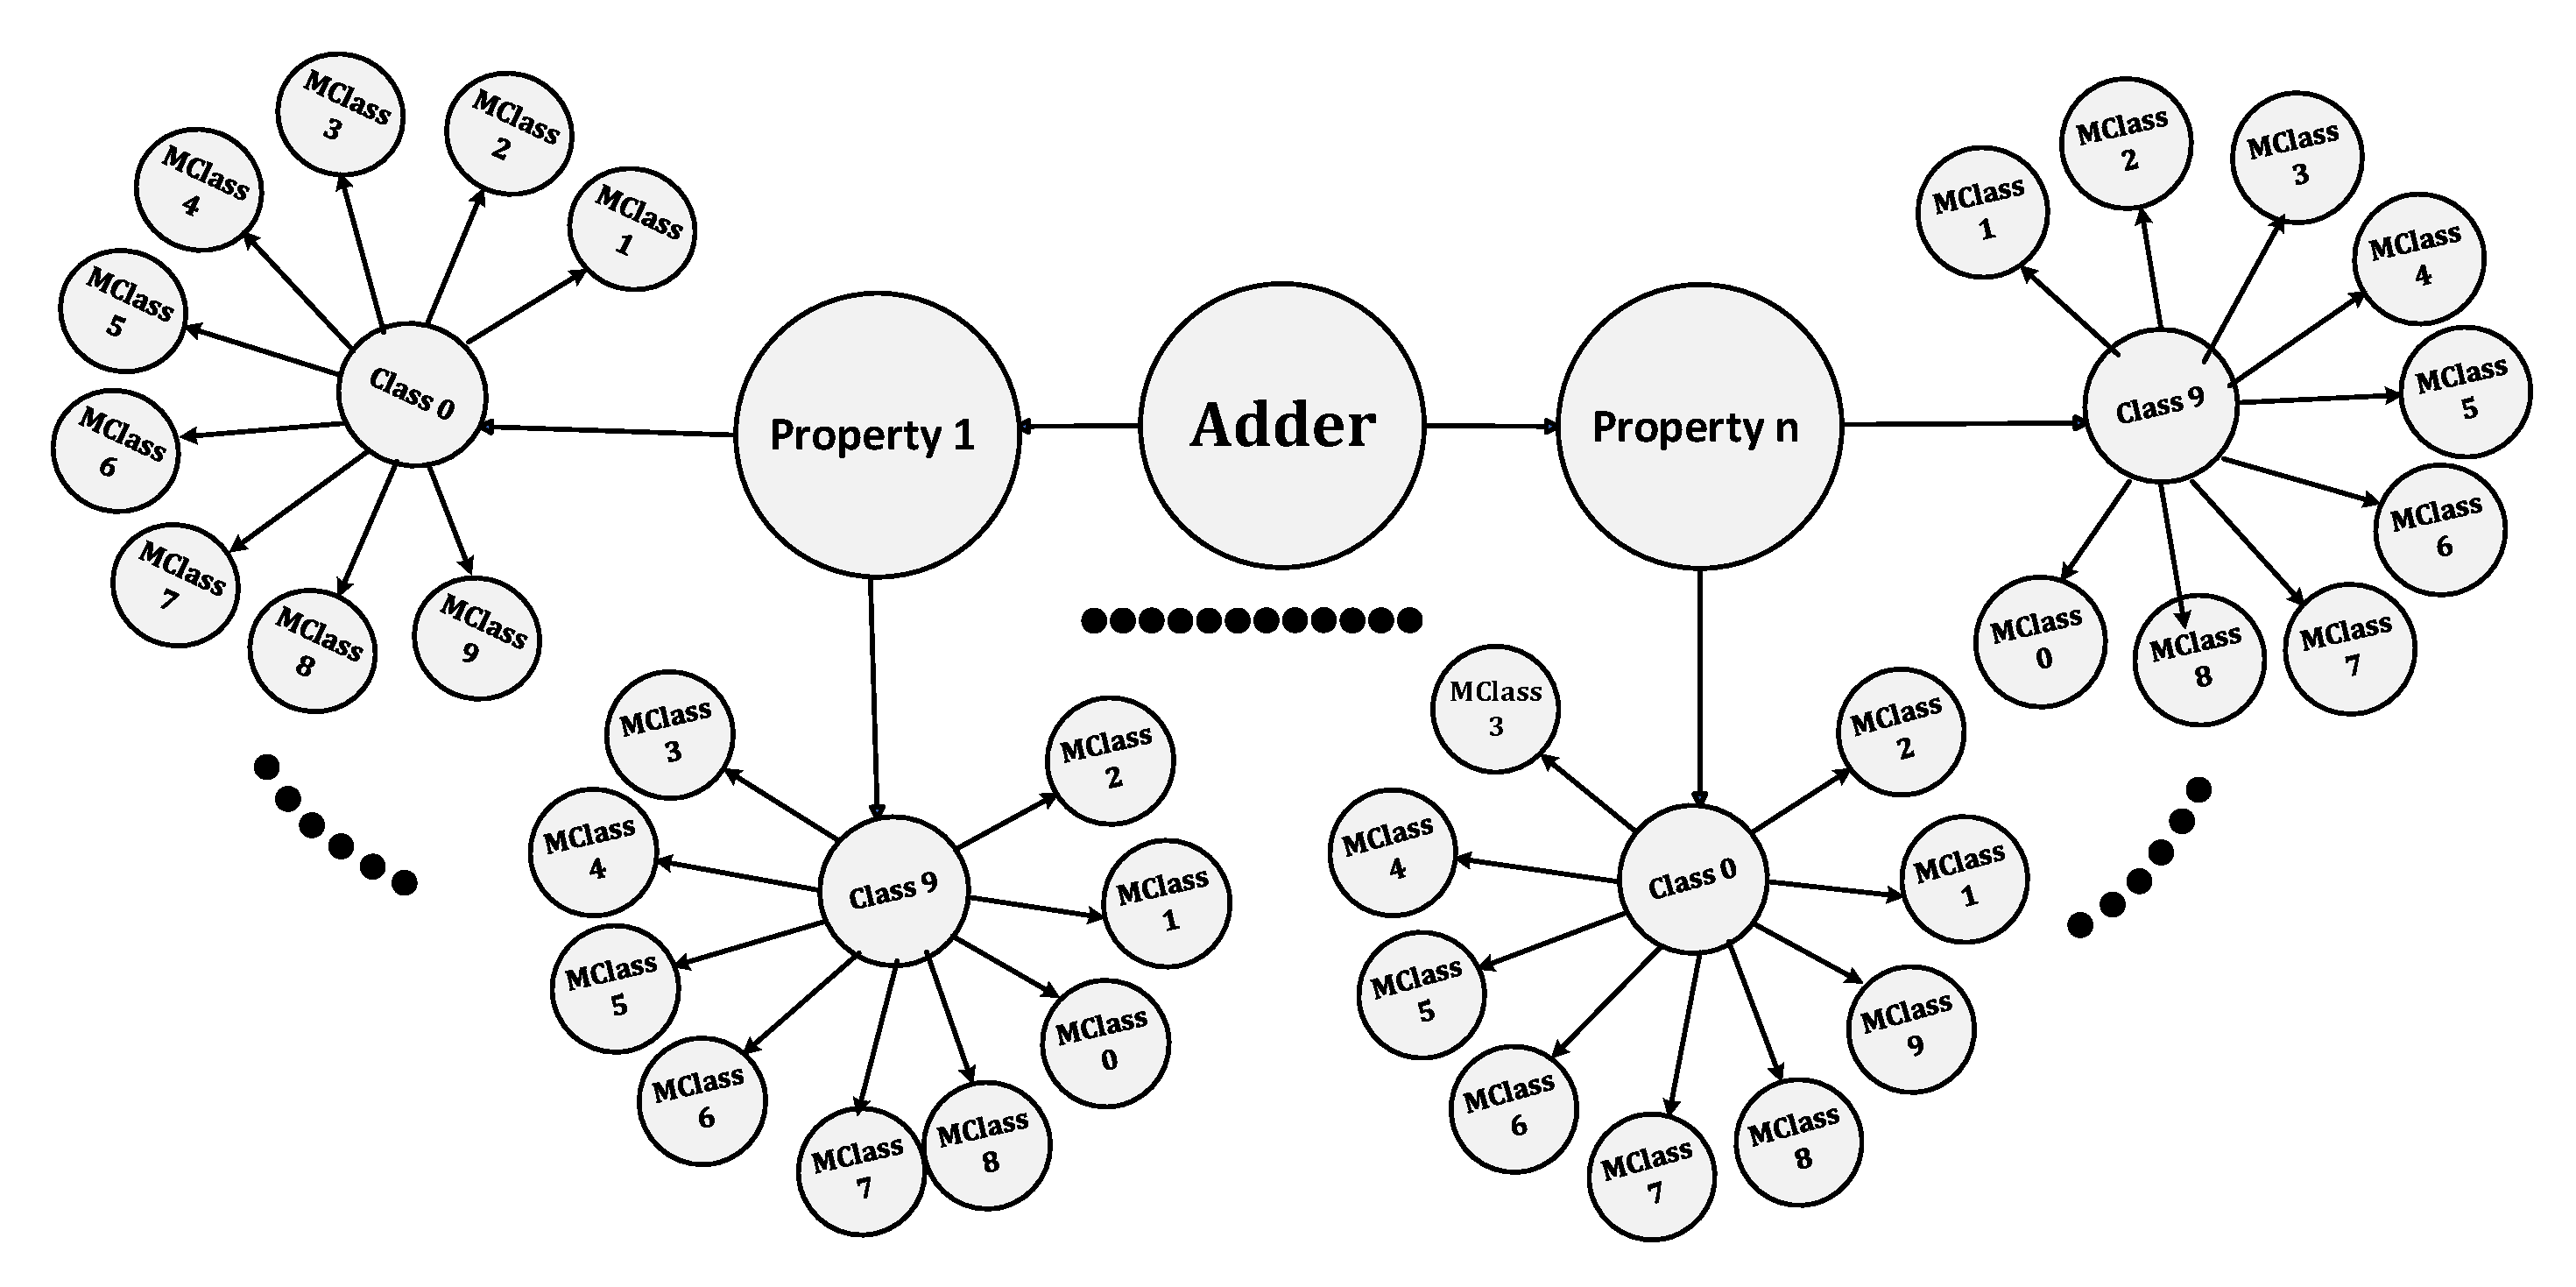
\includegraphics[width=1\textwidth]{figures/step5.pdf}
%     \caption{Error Summarization}
%     \label{Summarization}
% \end{figure*}

% \subsection{Use Cases and Examples}

% To illustrate the application of ProbLog for global robustness in real-world scenarios, we present the following use cases:

% \subsubsection{Use Case 1: Handwritten Digit Recognition}

% \textbf{Scenario:} Consider an AI system designed to recognize handwritten digits, such as the MNIST dataset. The system is evaluated under various transformations, including noise addition, rotation, and brightness adjustment. The goal is to determine the global robustness of the system in recognizing digit pairs correctly under these properties.

% The tables below provide the probabilities for correctly recognizing digit pairs under different conditions (AND and OR relationships) for an MNIST 2-digit addition system. Each world represents a different combination of transformations applied to the digits.

% \begin{table}[h]
%     \centering
%     \caption{Specification Probabilities for MNIST 2-Digit Addition Under Different Transformations}
%     \label{tab:mnist_prob_and_or}
%     \resizebox{\textwidth}{!}{%
%     \begin{tabular}{|c|c|c|c|c|c|}
%     \hline
%     \textbf{World} & \textbf{Conditions} & \textbf{Probability Expression (AND)} & \textbf{Probability (AND)} & \textbf{Probability Expression (OR)} & \textbf{Probability (OR)} \\
%     \hline
%     $w_1$ & \{noise(0), noise(1)\} & $0.85 \cdot 0.8$ & $0.68$ & $0.85 + 0.8 - (0.85 \cdot 0.8)$ & $0.97$ \\
%     $w_2$ & \{noise(0), correct(1)\} & $0.85 \cdot 0.9$ & $0.765$ & $0.85 + 0.9 - (0.85 \cdot 0.9)$ & $0.985$ \\
%     $w_3$ & \{correct(0), noise(1)\} & $0.9 \cdot 0.8$ & $0.72$ & $0.9 + 0.8 - (0.9 \cdot 0.8)$ & $0.98$ \\
%     $w_4$ & \{rotation(0), correct(1)\} & $0.88 \cdot 0.9$ & $0.792$ & $0.88 + 0.9 - (0.88 \cdot 0.9)$ & $0.992$ \\
%     $w_5$ & \{correct(0), rotation(1)\} & $0.9 \cdot 0.77$ & $0.693$ & $0.9 + 0.77 - (0.9 \cdot 0.77)$ & $0.977$ \\
%     $w_6$ & \{rotation(0), rotation(1)\} & $0.88 \cdot 0.77$ & $0.6776$ & $0.88 + 0.77 - (0.88 \cdot 0.77)$ & $0.9696$ \\
%     $w_7$ & \{noise(0), rotation(1)\} & $0.85 \cdot 0.77$ & $0.6545$ & $0.85 + 0.77 - (0.85 \cdot 0.77)$ & $0.9655$ \\
%     $w_8$ & \{rotation(0), noise(1)\} & $0.88 \cdot 0.8$ & $0.704$ & $0.88 + 0.8 - (0.88 \cdot 0.8)$ & $0.976$ \\
%     $w_9$ & \{correct(0), correct(1)\} & $0.9 \cdot 0.9$ & $0.81$ & $0.9 + 0.9 - (0.9 \cdot 0.9)$ & $0.99$ \\
%     \hline
%     \end{tabular}
%     }
% \end{table}

% \textbf{Explanation:} The table shows the global correctness probabilities for pairs of digits under various transformation conditions. Each row represents a different combination of transformations applied to the two digits in the pair:
% - AND Probability: The probability that both digits are correctly recognized under the specified transformations.
% - OR Probability: The probability that at least one of the digits is correctly recognized under the specified transformations.

% For example, in world $w_1$, both digits are subjected to noise, leading to an AND probability of $0.68$ and an OR probability of $0.97$.

% \textbf{Problog Code:}
% \begin{mdframed}[leftline=false, rightline=false, topline=true, bottomline=true]
% \scriptsize
% \begin{verbatim}
% % Define probabilities for digit 0 under different transformations
% 0.9::noise_0. % Digit 0 correctly predicted with 90% probability under noise
% 0.85::brightness_0. % Digit 0 correctly predicted with 85% probability under brightness
% 0.88::rotation_0. % Digit 0 correctly predicted with 88% probability under rotation

% % Define probabilities for digit 1 under different transformations
% 0.8::noise_1. % Digit 1 correctly predicted with 80% probability under noise
% 0.75::brightness_1. % Digit 1 correctly predicted with 75% probability under brightness
% 0.77::rotation_1. % Digit 1 correctly predicted with 77% probability under rotation

% % Define rules for correct prediction under each transformation for digit 0
% correct_noise_0 :- noise_0.
% correct_brightness_0 :- brightness_0.
% correct_rotation_0 :- rotation_0.

% % Define rules for correct prediction under each transformation for digit 1
% correct_noise_1 :- noise_1.
% correct_brightness_1 :- brightness_1.
% correct_rotation_1 :- rotation_1.

% % Define rules for incorrect prediction under each transformation for digit 0
% wrong_noise_0 :- +correct_noise_0.
% wrong_brightness_0 :- +correct_brightness_0.
% wrong_rotation_0 :- +correct_rotation_0.

% % Define rules for incorrect prediction under each transformation for digit 1
% wrong_noise_1 :- +correct_noise_1.
% wrong_brightness_1 :- +correct_brightness_1.
% wrong_rotation_1 :- +correct_rotation_1.

% % Define rules for correct prediction of both digits under noise
% pair_correct_noise_0_1 :- correct_noise_0, correct_noise_1.
% % Define rules for incorrect prediction of both digits under noise
% pair_wrong_noise_0_1 :- wrong_noise_0, wrong_noise_1.

% % Define global correctness based on either both correct or both incorrect under noise
% global_correct_noise_0_1 :- pair_correct_noise_0_1; pair_wrong_noise_0_1.

% % Query the global correctness under noise
% query(global_correct_noise_0_1).
% \end{verbatim}
% \end{mdframed}
% \captionof{figure}{Problog code snippet for evaluating handwritten digit recognition under noise, brightness, and rotation transformations.}

% \textbf{Explanation:} In this scenario, we are interested in the global correctness of recognizing pairs of digits (0 and 1) under different transformations. The ProbLog code models the local robustness probabilities for each transformation and combines them to evaluate the global correctness.

% \subsubsection{Use Case 2: Autonomous Vehicle Perception}

% \textbf{Scenario:} An AI system used in autonomous vehicles must reliably detect objects such as pedestrians and vehicles under various weather conditions (rain, fog, and snow). The goal is to evaluate the system's robustness in identifying these objects correctly under these weather conditions.

% \begin{mdframed}[leftline=false, rightline=false, topline=true, bottomline=true]
%   \scriptsize
%   \begin{verbatim}

% % Probabilities for Vehicle Detection under Different Weather Conditions
% 0.75::rain_vehicle. % Vehicle correctly detected with 75% probability under rain
% 0.55::fog_vehicle. % Vehicle correctly detected with 55% probability under fog
% 0.7::snow_vehicle. % Vehicle correctly detected with 70% probability under snow

% % Correct Detection Rules for Vehicle
% correct_rain_vehicle :- rain_vehicle.
% correct_fog_vehicle :- fog_vehicle.
% correct_snow_vehicle :- snow_vehicle.

% % Incorrect Detection Rules for Vehicle
% wrong_rain_vehicle :- +correct_rain_vehicle.
% wrong_fog_vehicle :- +correct_fog_vehicle.
% wrong_snow_vehicle :- +correct_snow_vehicle.

% % AND conditions for Vehicle Detection under all weather conditions
% global_correct_vehicle_and :- correct_rain_vehicle, correct_fog_vehicle, correct_snow_vehicle.

% % OR conditions for Vehicle Detection under any weather condition
% global_correct_vehicle_or :- correct_rain_vehicle; correct_fog_vehicle; correct_snow_vehicle.

% % Mixed conditions (AND & OR) for Vehicle Detection
% global_correct_mixed_vehicle :- correct_rain_vehicle, (correct_fog_vehicle; correct_snow_vehicle).

% % Queries for Global Correctness
% query(global_correct_vehicle_and).
% query(global_correct_vehicle_or).
% query(global_correct_mixed_vehicle).
% \end{verbatim}
% \end{mdframed}
% \captionof{figure}{Problog code snippet for evaluating vehicle detection under different weather conditions.}

% \textbf{Explanation:} The ProbLog code assesses the global robustness of the AI system in detecting objects (vehicles) under individual and combined weather conditions. This ensures that the system can reliably perform in diverse environmental scenarios.

% \begin{table}[h]
%   \centering
%   \caption{Specification Probabilities (AND) for Vehicle Detection Under Different Weather Conditions \\
%   \( P(A \cap B \cap C) = P(A) \times P(B) \times P(C) \)}
%   \label{tab:veh_prob_and}
%   \resizebox{\textwidth}{!}{%
%   \begin{tabular}{|c|c|c|c|}
%   \hline
%   \textbf{World} & \textbf{Conditions} & \textbf{Probability Expression (AND)} & \textbf{Probability (AND)} \\
%   \hline
%   $w_1$ & \{rain, fog\} & $0.75 \times 0.55$ & $0.4125$ \\
%   $w_2$ & \{rain, snow\} & $0.75 \times 0.7$ & $0.525$ \\
%   $w_3$ & \{rain, sand\} & $0.75 \times 0.6$ & $0.45$ \\
%   $w_4$ & \{fog, snow\} & $0.55 \times 0.7$ & $0.385$ \\
%   $w_5$ & \{fog, sand\} & $0.55 \times 0.6$ & $0.33$ \\
%   $w_6$ & \{snow, sand\} & $0.7 \times 0.6$ & $0.42$ \\
%   $w_7$ & \{rain, fog, snow\} & $0.75 \times 0.55 \times 0.7$ & $0.28875$ \\
%   $w_8$ & \{rain, fog, sand\} & $0.75 \times 0.55 \times 0.6$ & $0.2475$ \\
%   $w_9$ & \{rain, snow, sand\} & $0.75 \times 0.7 \times 0.6$ & $0.315$ \\
%   $w_{10}$ & \{fog, snow, sand\} & $0.55 \times 0.7 \times 0.6$ & $0.231$ \\
%   \hline
%   \end{tabular}
%   }
% \end{table}

% \textbf{Explanation:} This table shows the global correctness probabilities for detecting vehicles under different combinations of weather conditions using AND relationships. Each row represents a different combination of weather conditions applied to the detection scenario:
% - AND Probability: The probability that the vehicle is correctly detected under all specified weather conditions.

% For example, in world $w_1$, the vehicle detection system is subjected to rain and fog, leading to an AND probability of $0.4125$.

% \begin{table}[h]
%   \centering
%   \caption{Specification Probabilities (OR) for Vehicle Detection Under Different Weather Conditions \\
%   \( P(A \cup B \cup C) = P(A) + P(B) + P(C) - P(A \cap B) - P(A \cap C) - P(B \cap C) + P(A \cap B \cap C) \)}
%   \label{tab:veh_prob_or}
%   \resizebox{\textwidth}{!}{%
%   \begin{tabular}{|c|c|c|c|}
%   \hline
%   \textbf{World} & \textbf{Conditions} & \textbf{Probability Expression (OR)} & \textbf{Probability (OR)} \\
%   \hline
%   $w_1$ & \{rain; fog\} & $0.75 + 0.55 - (0.75 \times 0.55)$ & $0.8875$ \\
%   $w_2$ & \{rain; snow\} & $0.75 + 0.7 - (0.75 \times 0.7)$ & $0.925$ \\
%   $w_3$ & \{rain; sand\} & $0.75 + 0.6 - (0.75 \times 0.6)$ & $0.9$ \\
%   $w_4$ & \{fog; snow\} & $0.55 + 0.7 - (0.55 \times 0.7)$ & $0.835$ \\
%   $w_5$ & \{fog; sand\} & $0.55 + 0.6 - (0.55 \times 0.6)$ & $0.82$ \\
%   $w_6$ & \{snow; sand\} & $0.7 + 0.6 - (0.7 \times 0.6)$ & $0.88$ \\
%   $w_7$ & \{rain; fog; snow\} & $0.75 + 0.55 + 0.7 - (0.75 \times 0.55) - (0.75 \times 0.7) - (0.55 \times 0.7) + (0.75 \times 0.55 \times 0.7)$ & $0.966625$ \\
%   $w_8$ & \{rain; fog; sand\} & $0.75 + 0.55 + 0.6 - (0.75 \times 0.55) - (0.75 \times 0.6) - (0.55 \times 0.6) + (0.75 \times 0.55 \times 0.6)$ & $0.95125$ \\
%   $w_9$ & \{rain; snow; sand\} & $0.75 + 0.7 + 0.6 - (0.75 \times 0.7) - (0.75 \times 0.6) - (0.7 \times 0.6) + (0.75 \times 0.7 \times 0.6)$ & $0.967$ \\
%   $w_{10}$ & \{fog; snow; sand\} & $0.55 + 0.7 + 0.6 - (0.55 \times 0.7) - (0.55 \times 0.6) - (0.7 \times 0.6) + (0.55 \times 0.7 \times 0.6)$ & $0.938$ \\
%   \hline
%   \end{tabular}
%   }
% \end{table}

% \textbf{Explanation:} This table shows the global correctness probabilities for detecting vehicles under different combinations of weather conditions using OR relationships. Each row represents a different combination of weather conditions applied to the detection scenario:
% - OR Probability: The probability that the vehicle is correctly detected under at least one of the specified weather conditions.

% For example, in world $w_1$, the vehicle detection system is subjected to rain and fog, leading to an OR probability of $0.8875$.

% \section{Error Summarization}

% Error summarization involves evaluating the performance of the AI system by identifying and quantifying errors. We use Bayesian Network-based Coverage Metrics to assess both local and global coverage. Two testing coverage metrics are defined in Figure~\ref{Coverage}: local coverage (LC) and global coverage (GC).

% \begin{figure*}[h]
%     \centering
%     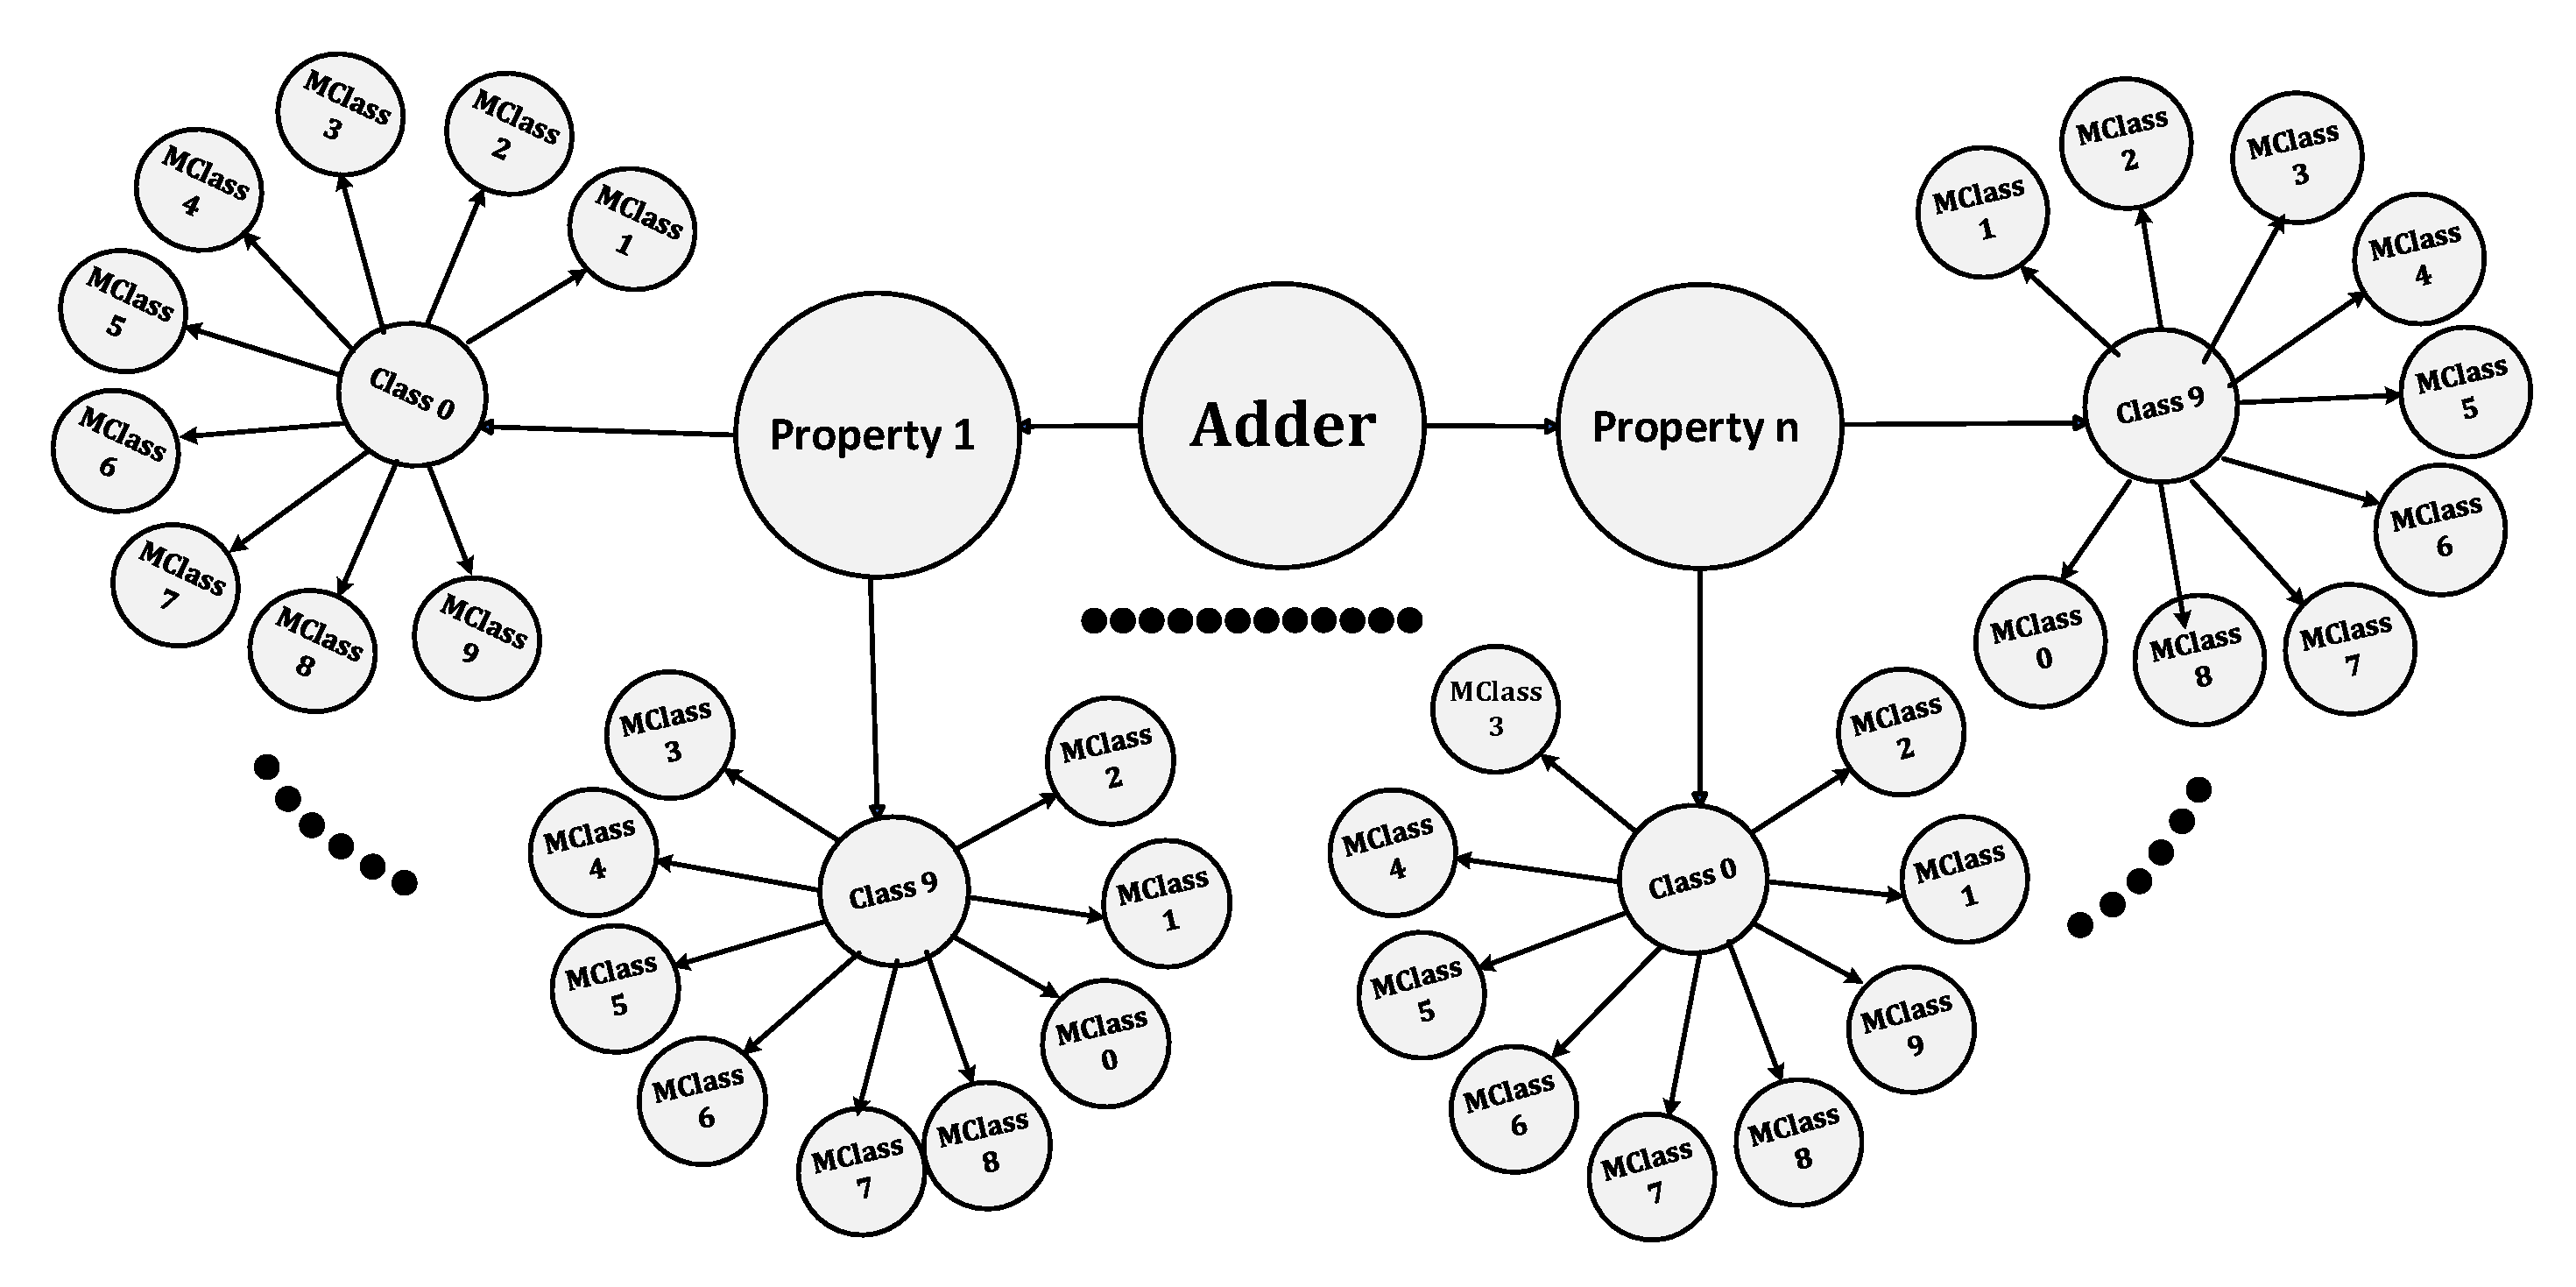
\includegraphics[width=\textwidth]{figures/step5.pdf}
%     \caption{Error Summarization}
%     \label{Summarization}
% \end{figure*}
\section{Error Summarization}

Error summarization involves evaluating the performance of the AI system by identifying and quantifying errors. We use Bayesian Network-based Coverage Metrics to assess both local and global coverage. Two testing coverage metrics are defined in Figure~\ref{Coverage}: local coverage (LC) and global coverage (GC).

\begin{figure*}[h]
    \centering
    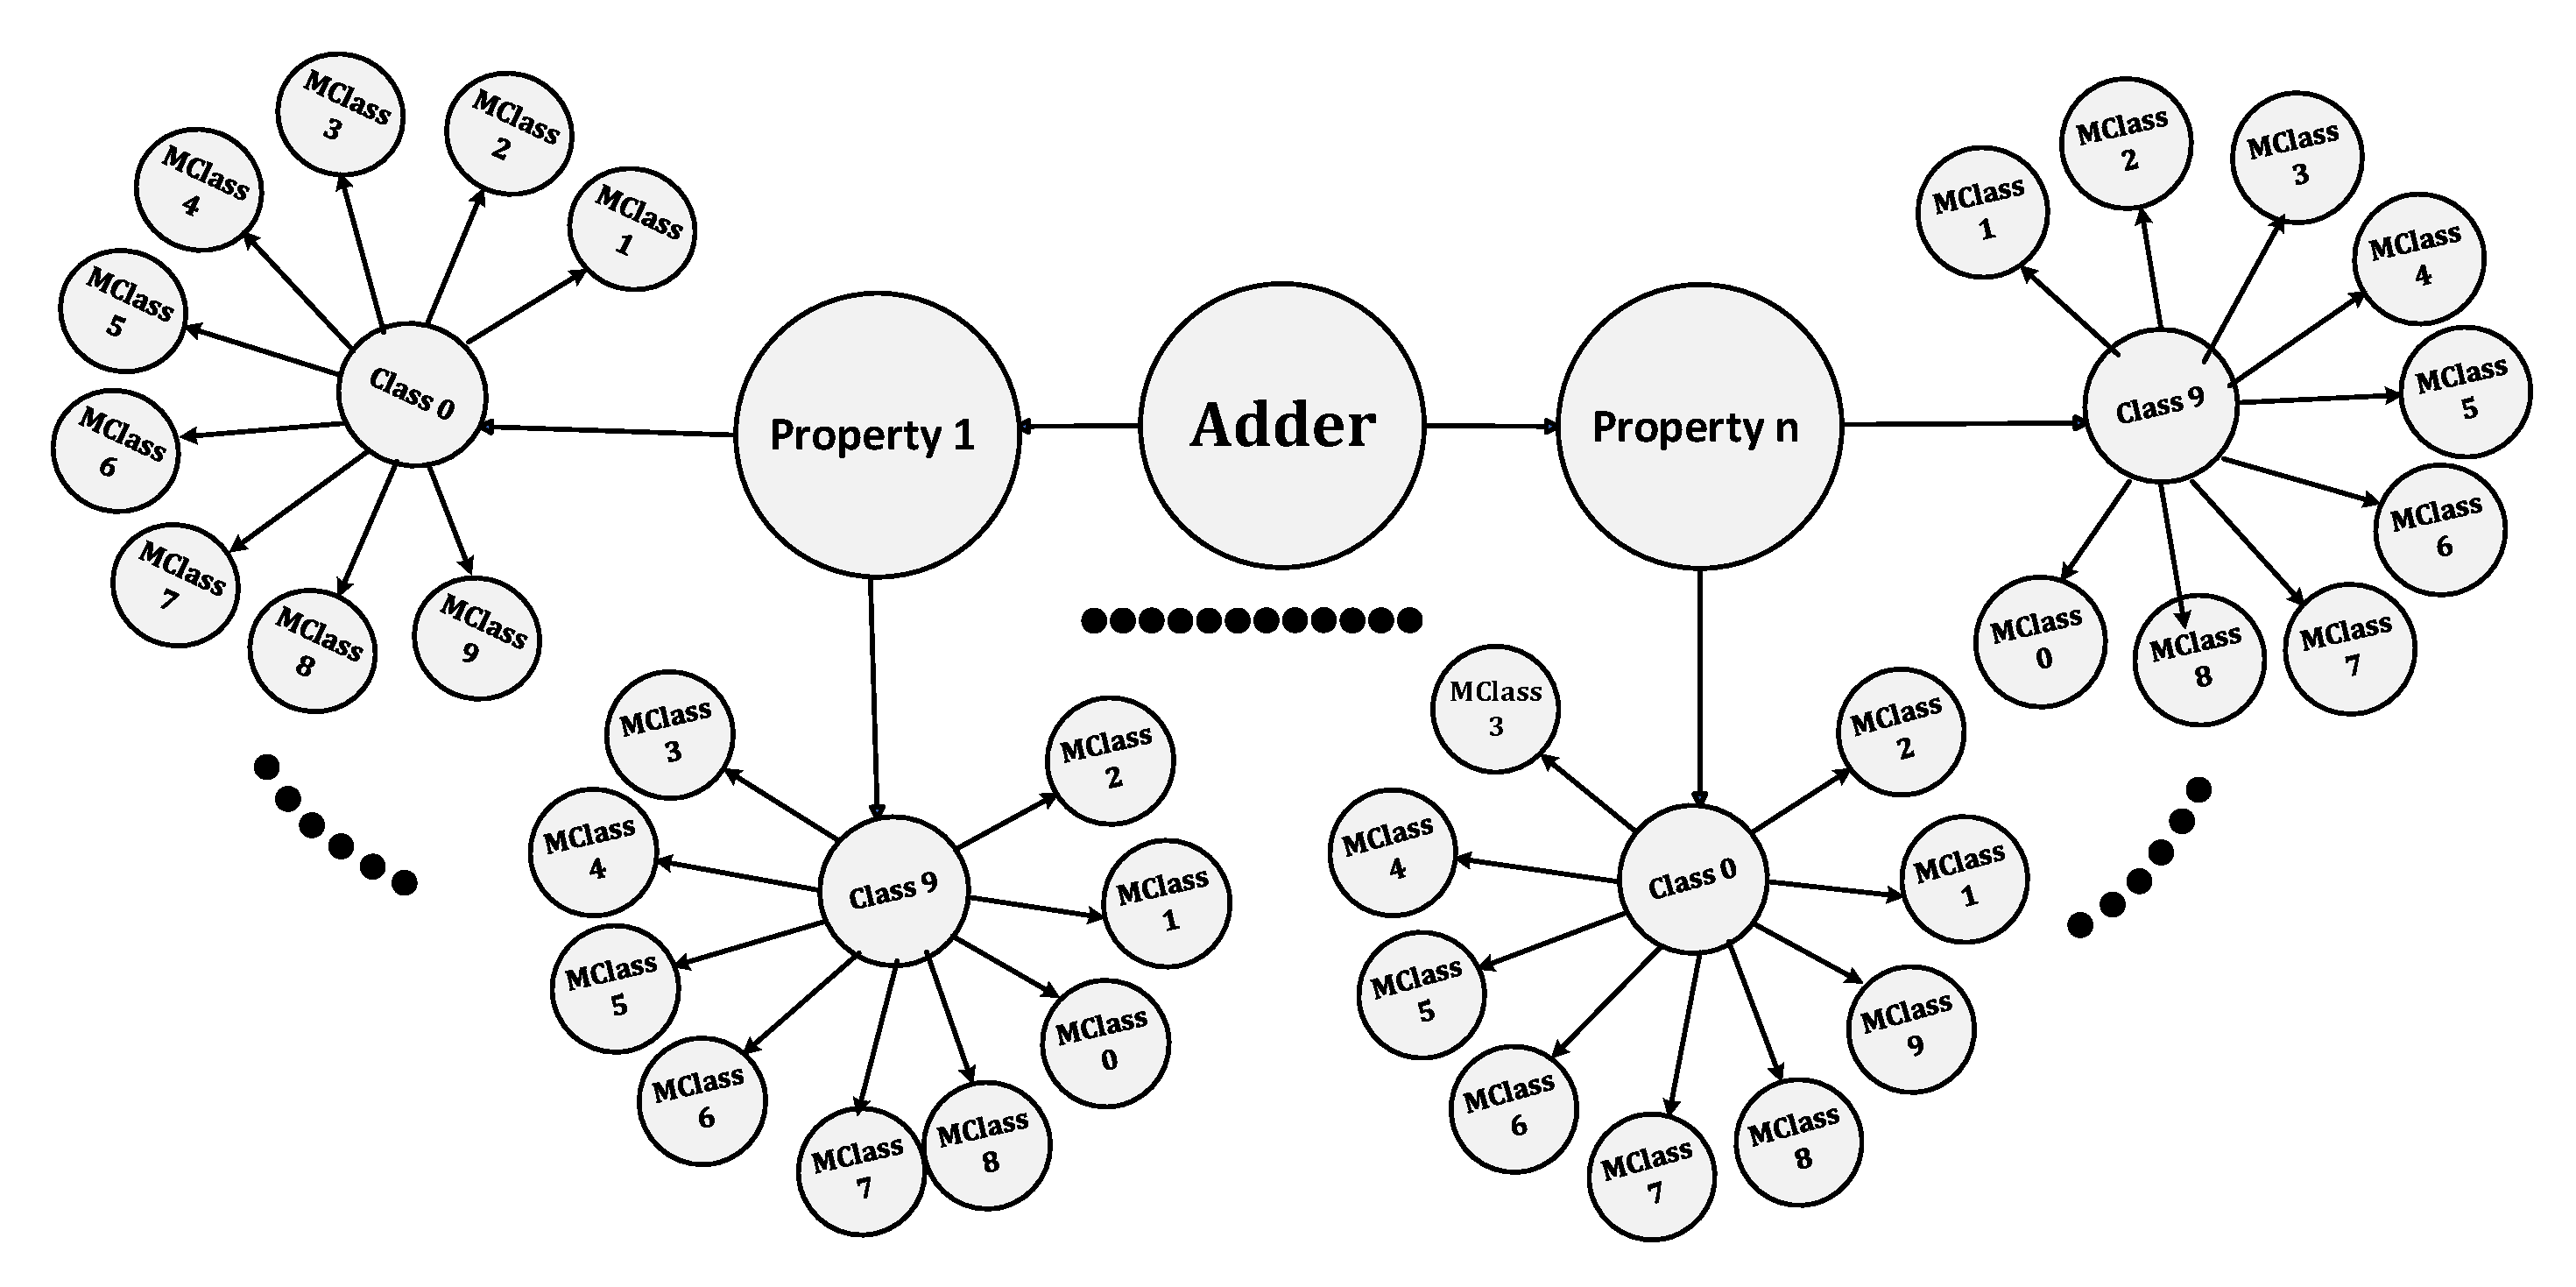
\includegraphics[width=\textwidth]{figures/step5.pdf}
    \caption{Error Summarization}
    \label{Summarization}
\end{figure*}



\section{Algorithm for Evaluating Model Robustness Using ProbLog}

\begin{algorithm}
  \caption{Evaluating Model Robustness Using ProbLog}
  \label{alg:model_robustness}
  \begin{algorithmic}[1]

  \REQUIRE $M$: Pre-trained model
  \REQUIRE $D$: Dataset
  \REQUIRE $N$: Number of samples per class
  \REQUIRE $P$: Set of properties

  \ENSURE $G$: Global correctness values for each specification

  \STATE \textbf{Load and Preprocess Data}
  \STATE $(X_{\text{train}}, y_{\text{train}}), (X_{\text{test}}, y_{\text{test}}) \leftarrow \text{load\_data}(D)$
  \STATE $X_{\text{test}} \leftarrow \text{preprocess\_data}(X_{\text{test}})$
  \STATE $\hat{Y} \leftarrow M.\text{predict}(X_{\text{test}})$
  \STATE $\hat{y} \leftarrow \text{extract\_predictions}(\hat{Y})$

  \STATE \textbf{Determine Number of Classes}
  \STATE $C \leftarrow \text{num\_classes}(y_{\text{test}})$ \COMMENT{Number of unique classes in the dataset}

  \STATE \textbf{Select Correctly Classified Samples}
  \STATE $\text{correct\_samples} \leftarrow \{ \}$
  \FOR{$c = 0$ \TO $C-1$} 
      \STATE $\text{correct\_samples}[c] \leftarrow \text{select\_correct\_samples}(X_{\text{test}}, y_{\text{test}}, \hat{y}, c, N)$
  \ENDFOR

  \STATE \textbf{Define Transformation Functions}
  \STATE $\text{define\_transformations}()$

  \STATE \textbf{Generate Test Cases}
  \FOR{$c = 0$ \TO $C-1$}
      \FORALL{$x \in \text{correct\_samples}[c]$}
          \FORALL{$T \in P$}
              \STATE $\text{generate\_test\_cases}(x, T)$
          \ENDFOR
      \ENDFOR
  \ENDFOR

  \STATE \textbf{Evaluate Model on Transformations}
  \FOR{$c = 0$ \TO $C-1$}
      \FORALL{$\text{property} \in P$}
          \STATE $L_{c, \text{property}} \leftarrow \text{compute\_accuracy}(M, \text{property}, c)$
      \ENDFOR
  \ENDFOR

  \STATE \textbf{Specification Definitions:}
  \STATE Specification1: $P(\text{Property1} \cap \text{Property2}) = P(\text{Property1}) \times P(\text{Property2})$ \COMMENT{AND relationship}
  \STATE Specification2: $P(\text{Property1} \cup \text{Property2}) = P(\text{Property1}) + P(\text{Property2}) - P(\text{Property1} \cap \text{Property2})$ \COMMENT{OR relationship}
  \STATE Specification3: Custom definitions
  \STATE \ldots

  \STATE \textbf{Generate and Evaluate ProbLog Code for Each Specification}
  \STATE Initialize $G$ as an empty list

  \FOR{$\text{spec} = 1$ \TO $\text{num\_specs}$}
      \STATE $\text{ProbLog Code}_{\text{spec}} \leftarrow \text{generate\_problog\_code}(L_{c, \text{property}}, \text{spec})$
      \STATE $G_{\text{spec}} \leftarrow \text{evaluate\_problog}(\text{ProbLog Code}_{\text{spec}})$
      \STATE Append $G_{\text{spec}}$ to $G$
  \ENDFOR

  \RETURN $G$
  \end{algorithmic}
\end{algorithm}


% Adjusting chapter title format for regular (numbered) chapters
\titleformat{\chapter}[display]
  {\normalfont\huge\bfseries\centering}{\chaptertitlename\ \thechapter}{20pt}{\Huge}

% Using similar styling for unnumbered chapters but without "Chapter" prefix
\titleformat{name=\chapter,numberless}
  {\normalfont\huge\bfseries\centering}{}{0pt}{\Huge}

\titlespacing*{\chapter}{0pt}{50pt}{40pt} % Adjust vertical spacing before and after the title


\chapter{Simulations and Results} % Ensures chapter numbering starts correctly

\label{chp:4}

\section{Datasets}


\subsection{MNIST Dataset}

The MNIST dataset is a widely recognized benchmark in the field of deep neural networks (DNNs), comprising 70,000 grayscale images of handwritten digits. These images are split into 60,000 training samples and 10,000 testing samples, each of size 28x28 pixels. The dataset includes labels for each digit from 0 to 9, making it a total of 10 classes. This dataset is extensively used for evaluating the performance of various DNN algorithms due to its simplicity and the well-established baseline results it offers. To ensure the correctness our model, we selected 100 correctly classified samples from each class. This selection process involved comparing the model's predictions with the actual labels and choosing only those samples where the predictions were correct. This resulted in a balanced subset of 1,000 samples, with 100 samples from each of the 10 classes.

\subsection{DAWN Dataset}

The DAWN (Vehicle Detection in Adverse Weather Nature Dataset) dataset focuses on vehicle detection under adverse weather conditions, providing a diverse set of real-traffic images categorized into four weather conditions: fog, snow, rain, and sandstorms. Initially, the class distribution in the training set was imbalanced, with the following counts: 258 for label 1, 240 for label 0, 163 for label 3, and 160 for label 2.

To address this imbalance, we resampled the training set to ensure an equal number of samples for each class. This resulted in a balanced training set with 258 samples for each label. This balancing step was crucial for fair training and evaluation of the model, ensuring that no class was overrepresented or underrepresented.

For the testing set, we selected 100 samples from each class, ensuring a balanced evaluation dataset. This selection process was critical to accurately assess the model's performance across different classes and adverse weather conditions.




\section{Use Case 1: Handwritten Digit Recognition }
\subsection{Local Correctness Evaluation}

In this section, we evaluate the local correctness of the model under different transformations, namely rotation, noise, and brightness. Each transformation is applied with specific parameters to simulate real-world variations. Images are rotated by 25 degrees to evaluate the model's performance under rotation. Gaussian noise with a noise factor of 0.2 is added to the images to test the model's robustness to noisy conditions. The brightness of the images is increased by a factor of 0.3 to simulate different lighting conditions.

The local correctness graphs provide insights into the model's robustness under these transformations for each digit class. The model exhibited high performance under rotation (0.99) and brightness (1.00) for Class 0, with slightly reduced accuracy under noise (0.81). For Class 1, the model maintained consistently high accuracy across all transformations: rotation (0.99), noise (0.99), and brightness (1.00). However, the model struggled more with rotations (0.76) and noise (0.79) for Class 2 compared to brightness (1.00). Similarly, for Class 3, the model showed lower accuracy for rotations (0.82) and noise (0.78), but performed perfectly under brightness (1.00). 

Class 4 demonstrated high accuracy across all properties, with rotation (0.91), noise (0.86), and brightness (1.00). Class 5 maintained high performance under all transformations: rotation (0.89), noise (0.99), and brightness (1.00). The model showed noticeable difficulty with noise (0.64) for Class 6, while maintaining high accuracy for rotation (0.87) and brightness (0.99). For Class 7, high accuracy was observed under brightness (1.00), with reduced performance under rotation (0.75) and noise (0.86). The model faced significant challenges under noise (0.02) for Class 8, but maintained good performance for rotation (0.68) and brightness (0.99). Finally, for Class 9, the model showed moderate performance under noise (0.51), and high accuracy under rotation (0.93) and brightness (0.99).

Overall, the model demonstrates strong robustness to brightness changes across all classes, frequently achieving perfect accuracy. However, performance under noise is highly variable, with some classes, such as Class 8, experiencing a dramatic drop in accuracy. While the model generally handles rotations well, there remains room for improvement, particularly in addressing noise-induced challenges. This analysis highlights the necessity for targeted training to enhance the model's robustness, especially under noisy conditions for specific classes.

\begin{figure}[h]
    \centering
    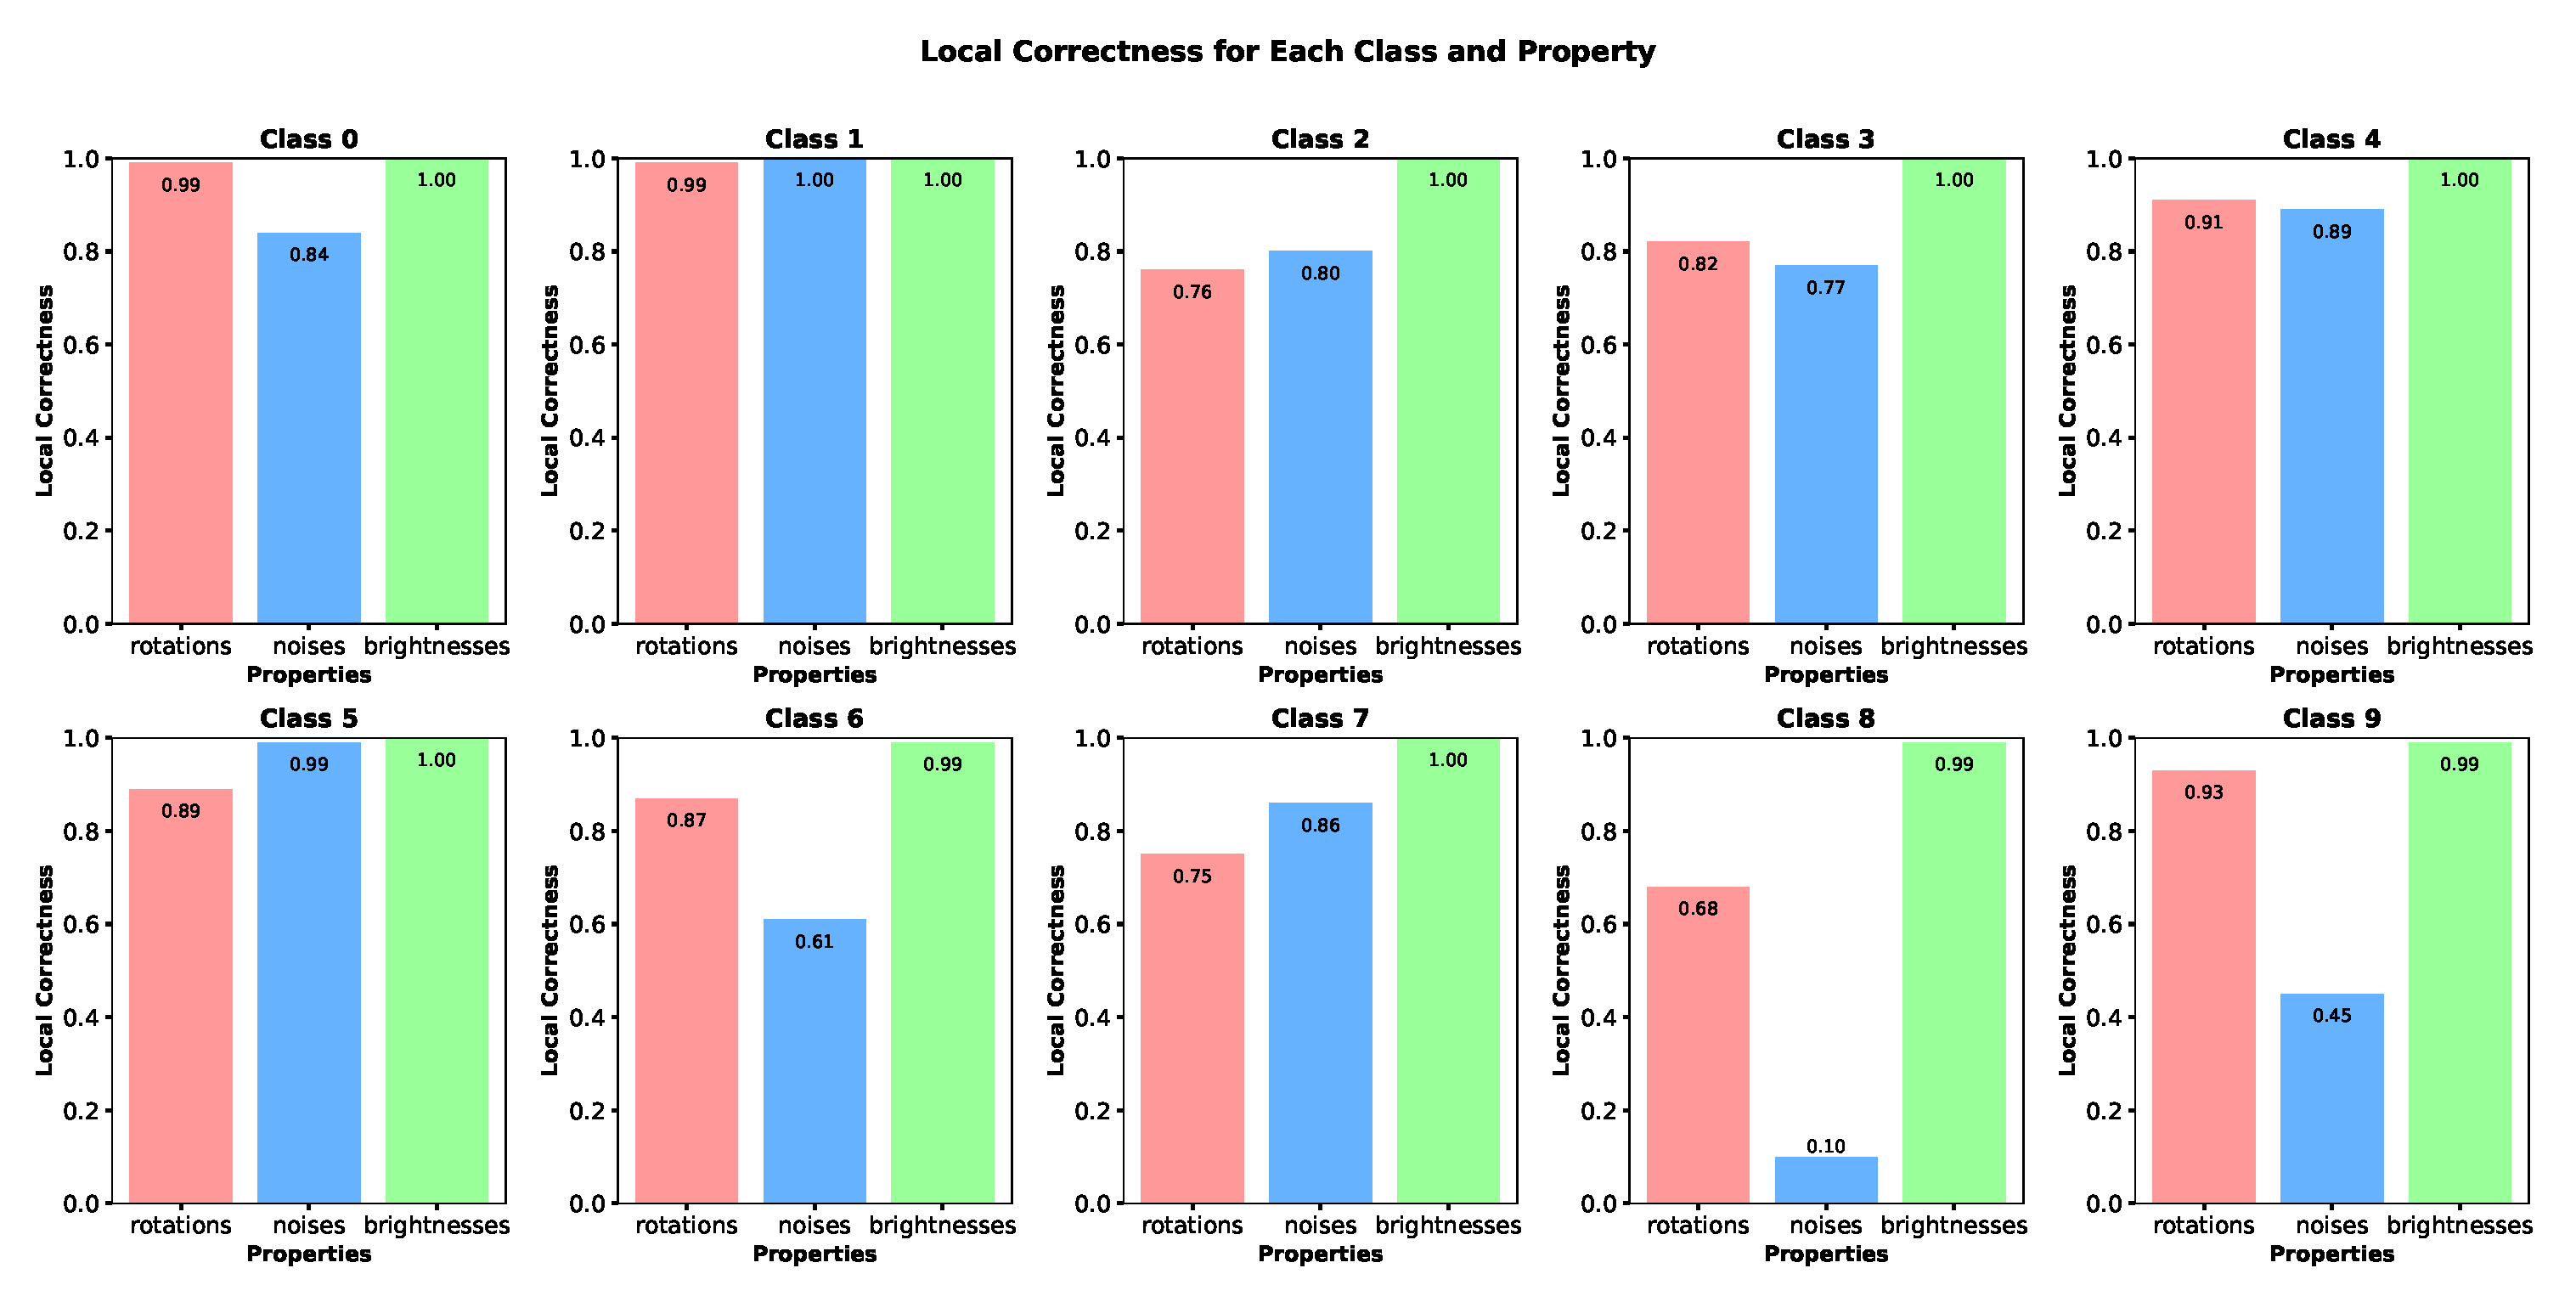
\includegraphics[width=\textwidth]{local_correctness.eps}
    \caption{Local Correctness for each Class and Property}
    \label{fig:local_correctness}
\end{figure}
\subsection{Global Correctness Evaluation}
The following figures illustrate the global correctness of various pairs of digits under different transformations: noise, brightness adjustment, and rotation. The final global correctness for each transformation is also depicted.

In my experiment, I checked the following specifications:

\scalebox{0.9}{%
\begin{minipage}{\linewidth}
\begin{align*}
  global\_noise &\leftrightarrow (noise\_0\_0 \land noise\_0\_1 \land noise\_0\_2 \land \ldots \land noise\_9\_9) \\
  global\_brightness &\leftrightarrow (brightness\_0\_0 \land brightness\_0\_1 \land brightness\_0\_2 \land \ldots \land brightness\_9\_9) \\
  global\_rotation &\leftrightarrow (rotation\_0\_0 \land rotation\_0\_1 \land rotation\_0\_2 \land \ldots \land rotation\_9\_9) \\
  global\_system &\leftrightarrow (global\_noise \lor global\_brightness \lor global\_rotation)
\end{align*}
\end{minipage}
}
  


\begin{figure}[H]
    \centering
    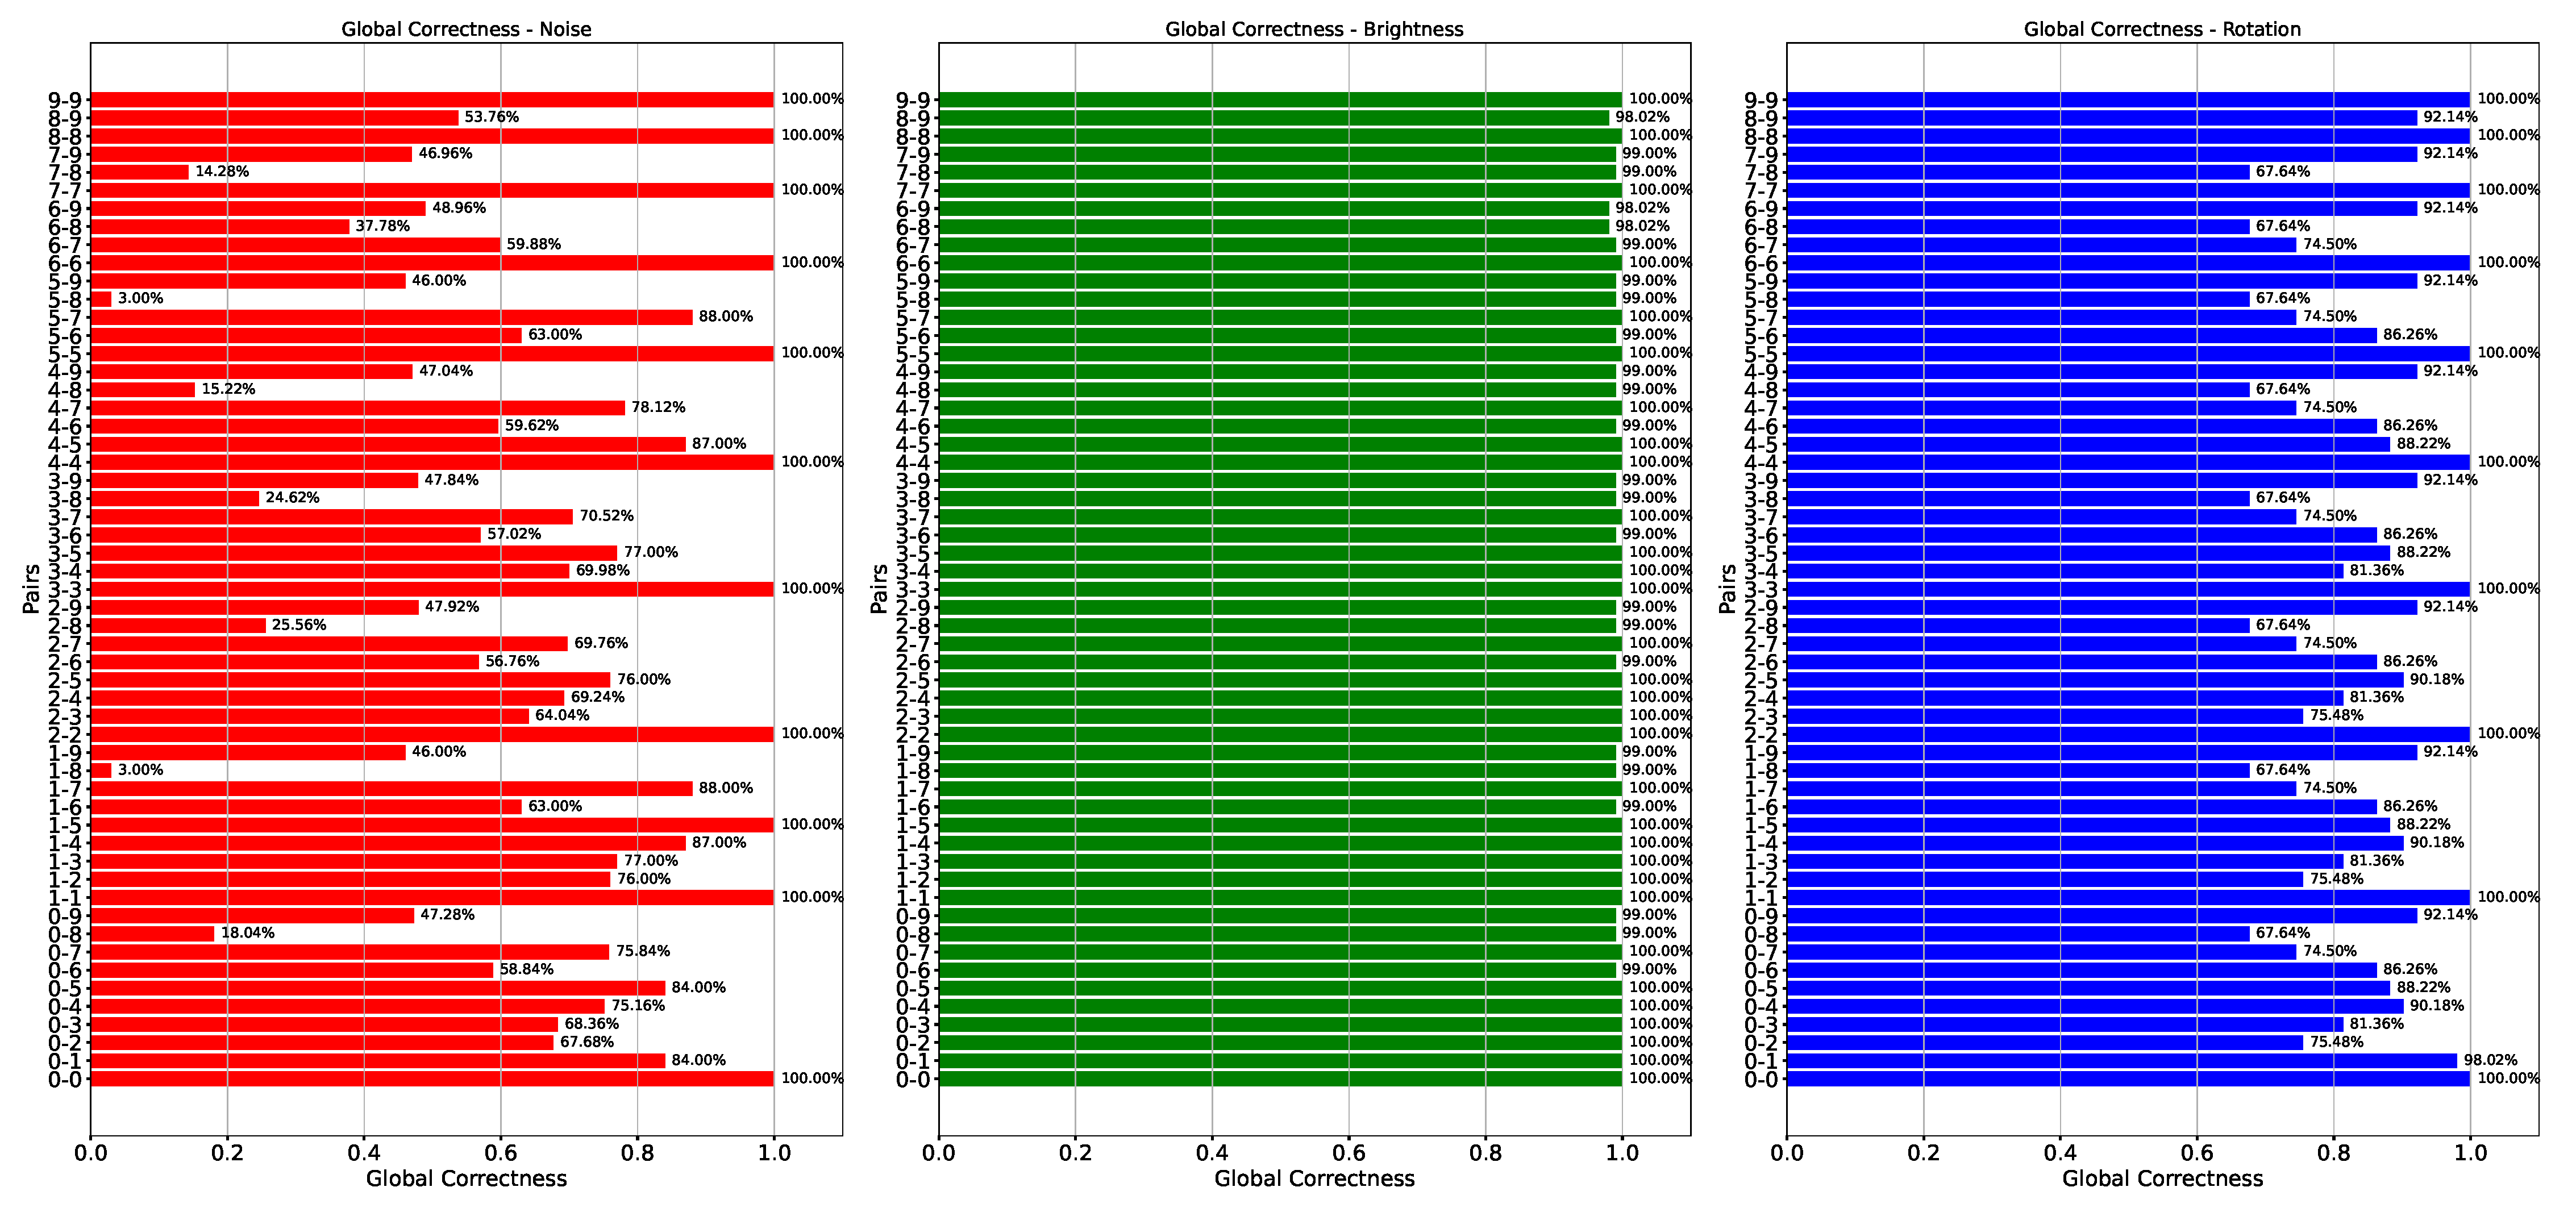
\includegraphics[width=\textwidth]{global_correctness.eps}
    \caption{Global Correctness for Noise, Brightness, and Rotation Transformations}
    \label{fig:global_correctness}
\end{figure}

\begin{figure}[H]
    \centering
    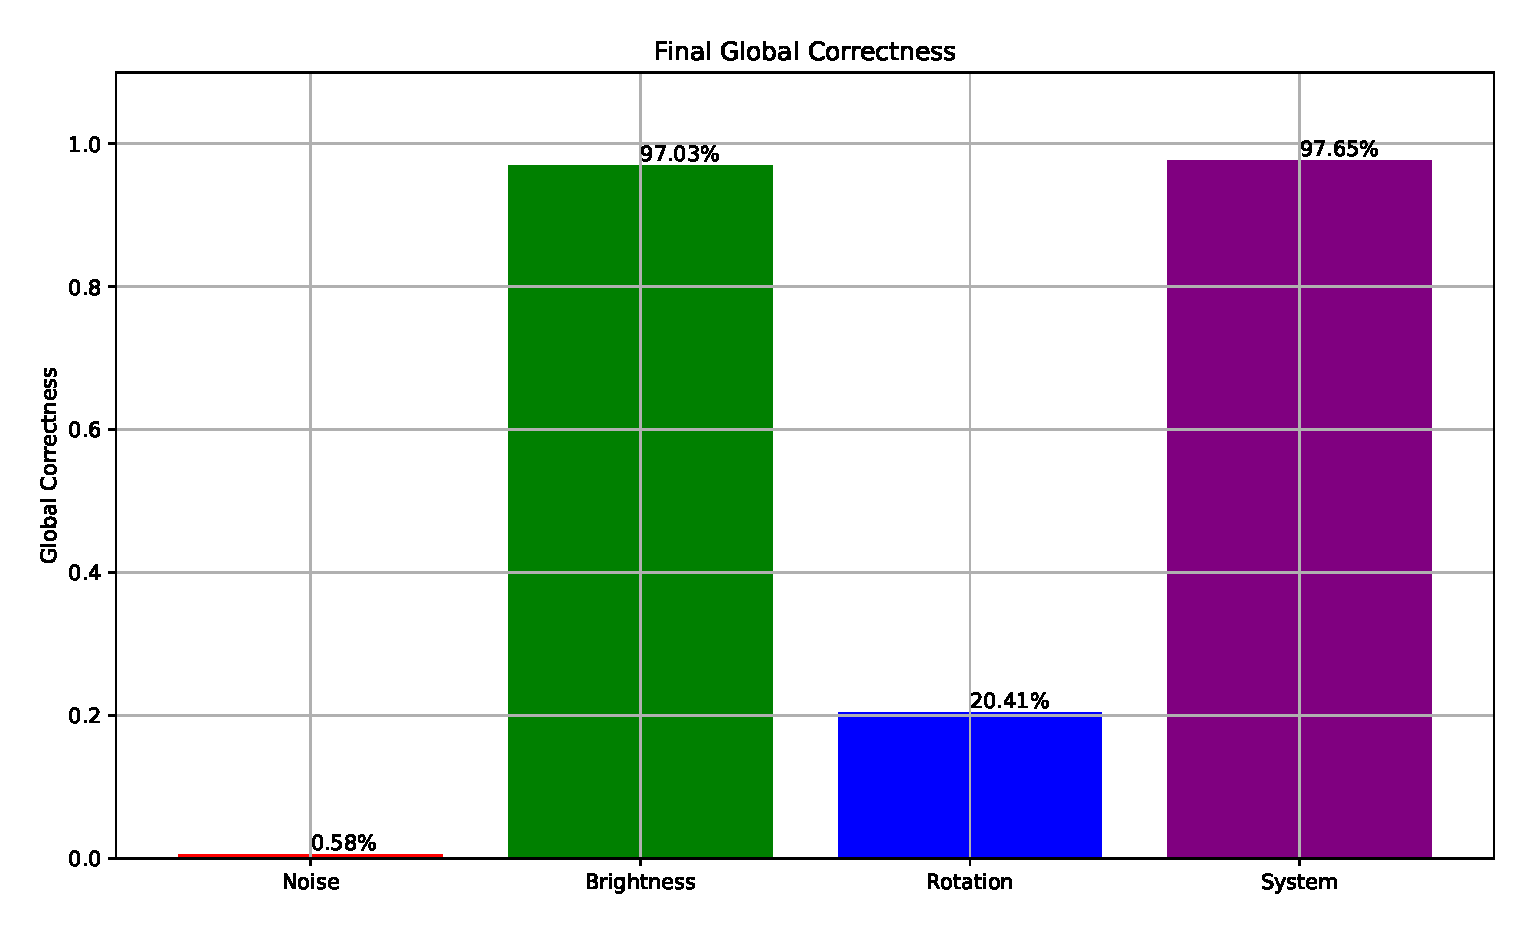
\includegraphics[width=0.8\textwidth]{global_correctness_combine.eps}
    \caption{Final Global Correctness}
    \label{fig:final_global_correctness}
\end{figure}

The global correctness values for pairs of digits under the noise transformation vary significantly. Some pairs such as (0,0), (1,1), (2,2), etc., achieve perfect correctness (100\%), while others like (0,5) and (1,8) exhibit very low correctness (3.00\% and 18.04\%, respectively). This indicates that the model's performance is highly inconsistent under noise, likely due to the distortion introduced affecting digit recognition. The model performs exceptionally well under brightness adjustments, with most pairs achieving near-perfect correctness. This suggests that the model is robust to changes in brightness, maintaining high confidence scores despite variations in image illumination. Performance under rotation is moderate, with significant variations across different pairs. Some pairs like (0,0), (1,1), (3,3), etc., achieve high correctness, while others such as (2,5) and (5,8) have lower correctness values. This variation suggests that while the model can handle certain rotations well, it struggles with others, potentially due to the angles and the inherent difficulty in recognizing rotated digits.

Combining the global correctness across all transformations, we observe an overall high performance with a final global correctness of 97.65\%. **Brightness** contributes the most to this high score (97.03\%), while Noise contributes the least (0.58\%). Rotation has a moderate impact (20.41\%), reflecting its varied performance across different pairs. These observations highlight the strengths and weaknesses of the AI subsystem under different transformations. The high performance under brightness adjustments indicates robustness to illumination changes, while the challenges with noise and rotation suggest areas for improvement in handling these perturbations.


\section{Use Case 2: Autonomous Vehicle Perception}

In this use case, we investigate the robustness of an AI system for autonomous vehicles in detecting objects, particularly vehicles, under various weather conditions including fog, rain, snow, and sand. The goal is to assess the system's performance across these challenging environments to ensure reliable operation.

The dataset was split into training and validation sets, with class balancing performed through oversampling to address any class imbalances. Data augmentation techniques such as rotation, width and height shifts, shear transformation, zoom, and horizontal flips were applied to the training set to enhance the model's generalizability.

The trained model's performance was evaluated on a balanced validation set resampled to ensure uniform class distribution.

\subsection{Local Correctness Analysis}

The local correctness of the model for each weather condition is depicted in the first graph. The AI system exhibits the following correctness values:
- \textbf{Fog:} The detection correctness is 51\%, indicating moderate performance. Fog conditions likely introduce significant visual obstructions that challenge the model's ability to correctly identify vehicles.
- \textbf{Rain:} Achieving a correctness of 75\%, the model performs relatively well in rainy conditions, suggesting robustness to moderate visual disturbances caused by rain.
- \textbf{Snow:} Similar to rain, the system shows a correctness of 75\%, demonstrating its capability to handle snowy environments, where the visual contrast might be reduced.
- \textbf{Sand:} With the highest correctness of 88\%, the model excels in sandy conditions, possibly due to clearer visibility compared to other adverse weather scenarios.

\subsection{Global Correctness Analysis}

\subsection{Global Correctness Evaluation for Vehicle Detection}

The second graph illustrates the global correctness for vehicle detection under different combination methods of weather conditions:

\scalebox{0.9}{%
\begin{minipage}{\linewidth}
\begin{align*}
  global\_weather &\leftrightarrow (fog \land rain \land snow \land sand) \\
  global\_weather &\leftrightarrow (fog \lor rain \lor snow \lor sand) \\
  global\_weather &\leftrightarrow (fog \land (rain \lor snow \lor sand))
\end{align*}
\end{minipage}
}

\begin{figure}[h]
  \centering
  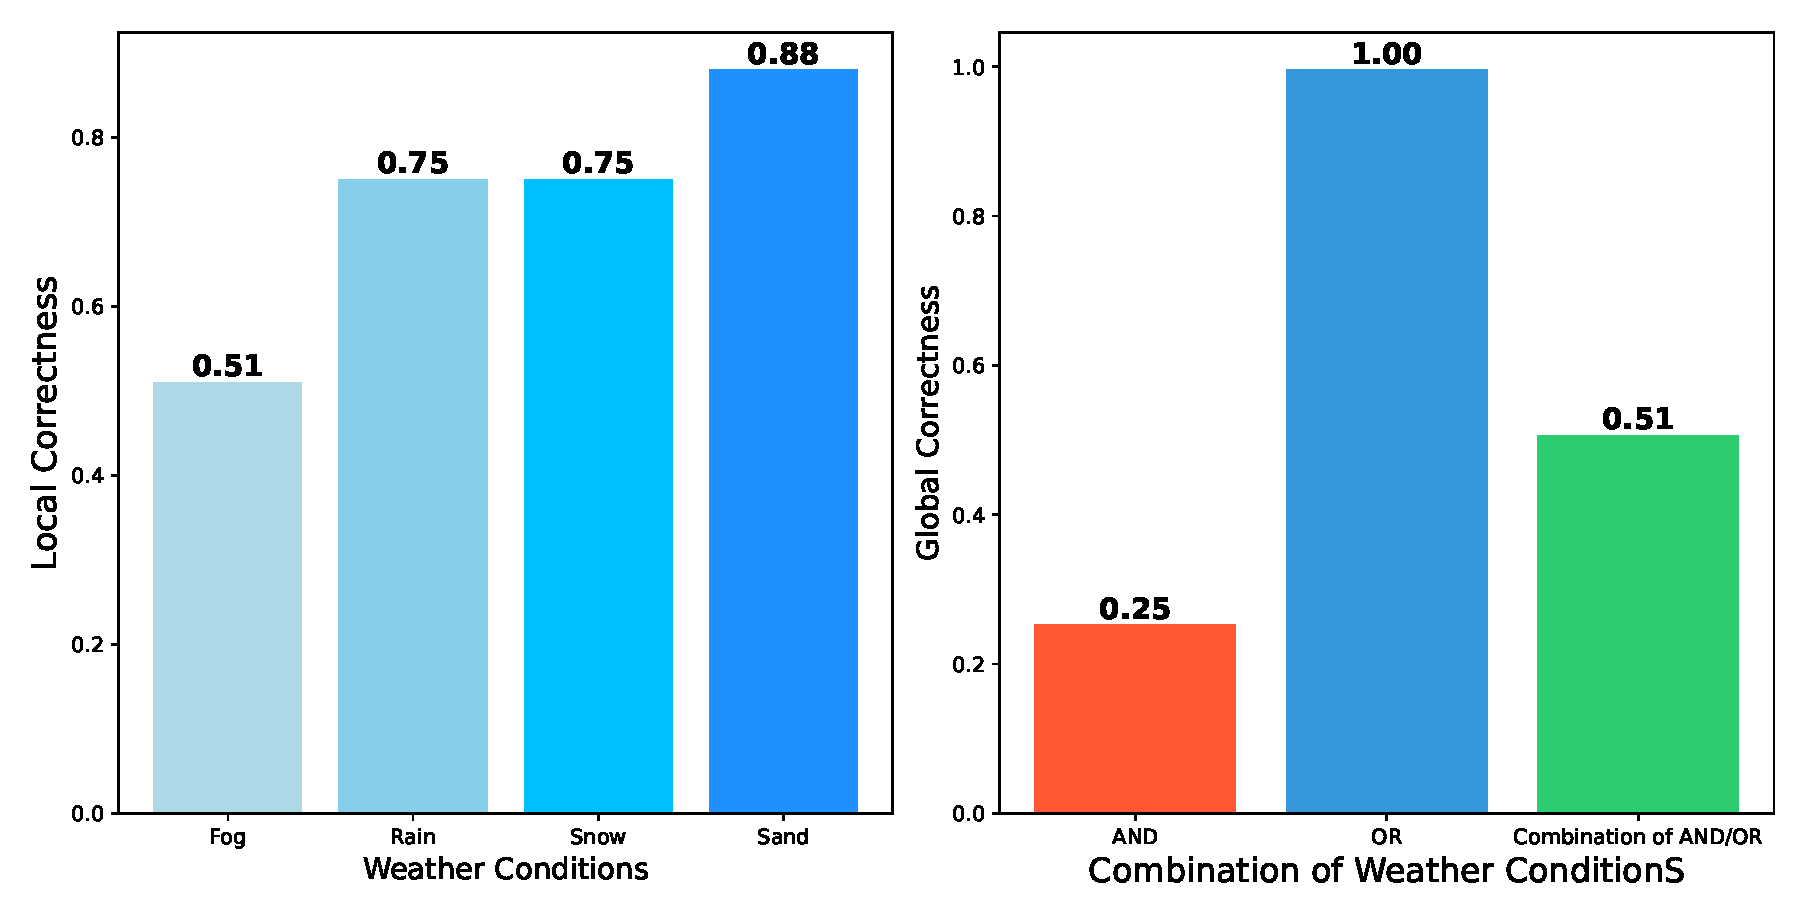
\includegraphics[width=0.8\textwidth]{globalcorrectness_vehicle_detection.eps}
  \caption{Local and Global Correctness of Vehicle Detection Under Various Weather Conditions}
  \label{fig:global_correctness_vehicle_detection}
\end{figure}




\begin{itemize}
    \item \textbf{AND (Intersection):} The model's correctness is 25\%. This low value reflects the stringent requirement for the system to correctly detect vehicles under all specified conditions simultaneously, highlighting potential vulnerabilities when multiple weather challenges are present.
    \item \textbf{OR (Union):} Achieving a perfect correctness of 100\%, the model successfully detects vehicles under at least one of the conditions. This high performance underscores the system's reliability when at least one favorable condition is present.
    \item \textbf{Combination of AND/OR:} The correctness stands at 51\%, representing a balanced approach where the model must correctly detect vehicles under fog and any one of the other conditions (rain, snow, or sand). This mixed strategy provides a realistic measure of the system's robustness in practical scenarios with varying weather conditions.
\end{itemize}



\newpage

%results

%% Adjusting chapter title format for regular (numbered) chapters
\titleformat{\chapter}[display]
  {\normalfont\huge\bfseries\centering}{\chaptertitlename\ \thechapter}{20pt}{\Huge}

% Using similar styling for unnumbered chapters but without "Chapter" prefix
\titleformat{name=\chapter,numberless}
  {\normalfont\huge\bfseries\centering}{}{0pt}{\Huge}

\titlespacing*{\chapter}{0pt}{50pt}{40pt} % Adjust vertical spacing before and after the title

\definecolor{barblue}{RGB}{153,204,254}
\definecolor{groupblue}{RGB}{51,102,254}
\definecolor{linkred}{RGB}{165,0,33}
\chapter{PhD Two-Year Plan} % Ensures chapter numbering starts correctly
\label{chp:9}

\section{Research Modules}
I have categorized my research into seven modules as depicted in Figure \ref{fig:no_publish}: Module 1 (DNN Testing Framework), Module 2 (Specification), Module 3 (Sampling), Module 4 (Interpretability), Module 5 (Testcase Generation), Module 6 (Coverage Criteria), and Module 7 (Error Summarization).

\begin{figure}[ht]
  \centering
  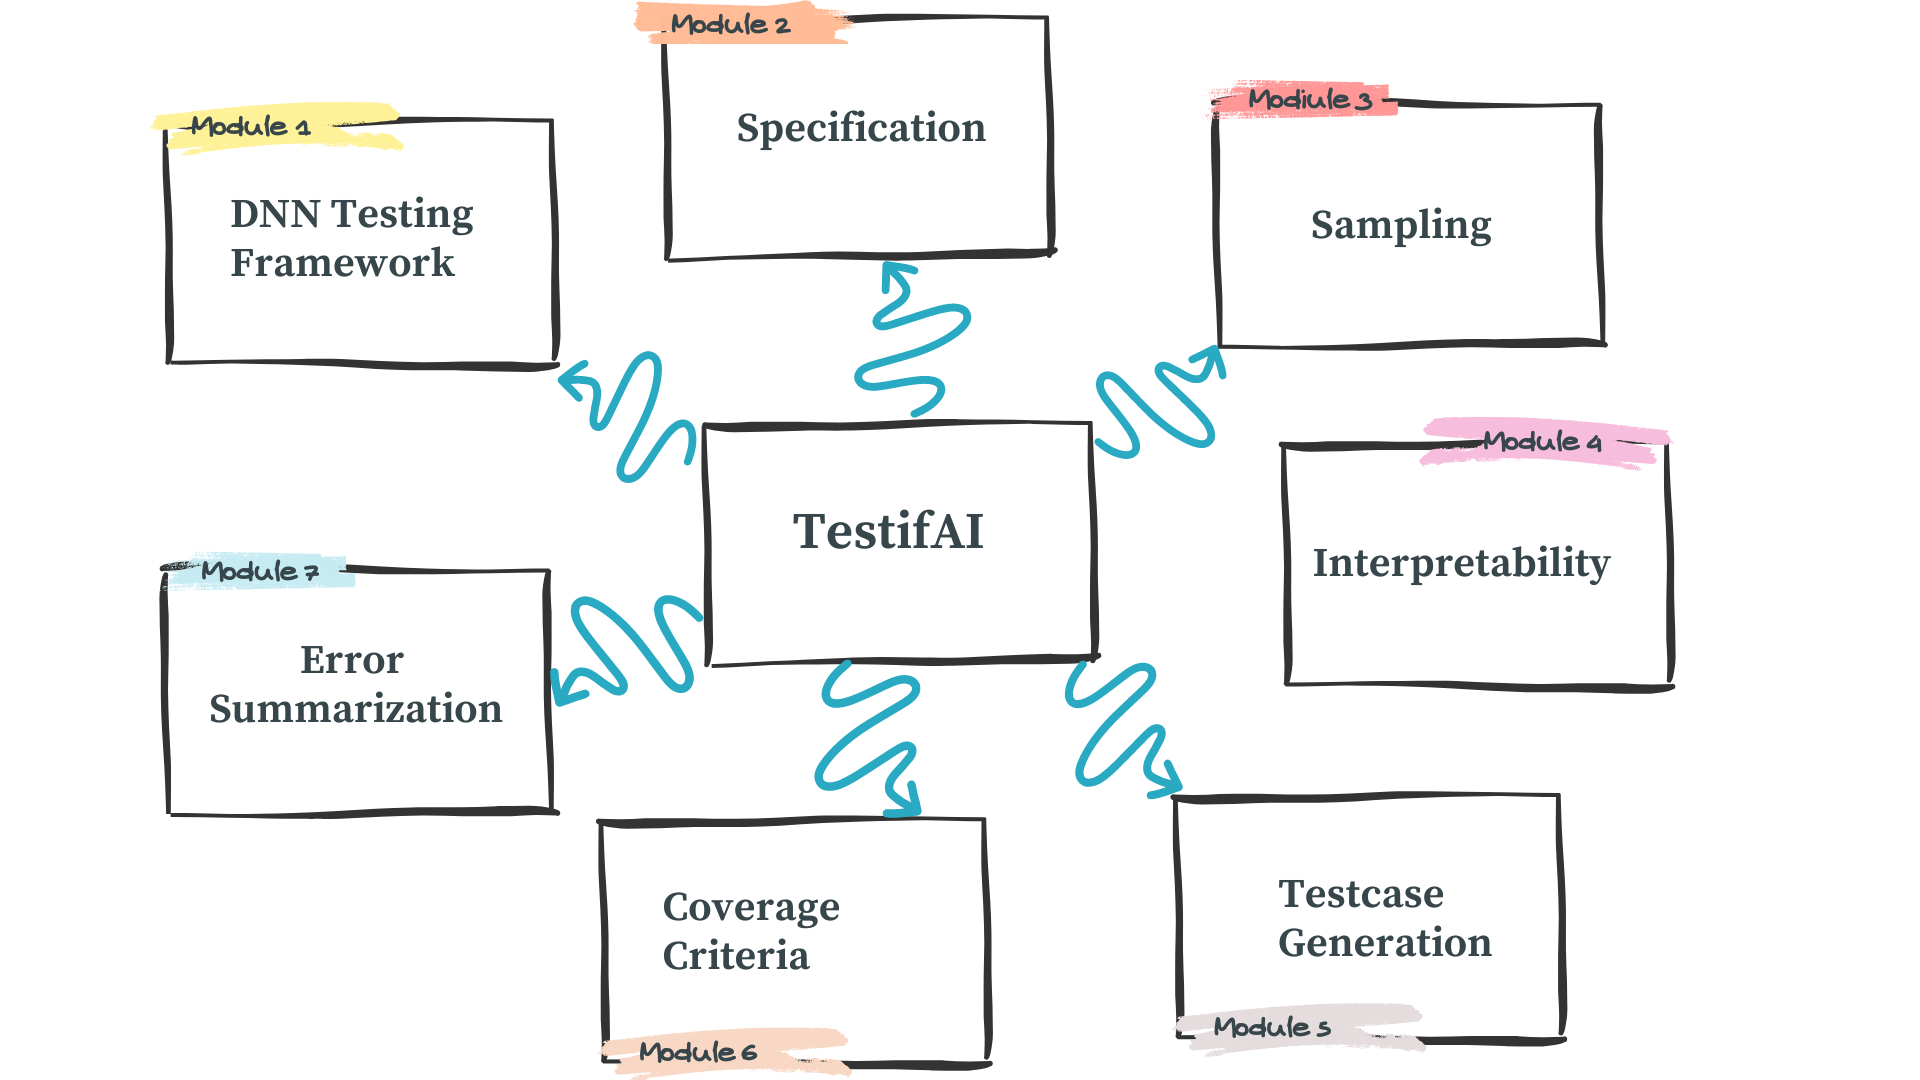
\includegraphics[width=\linewidth]{researchareas.png}
  \caption{Research Modules}
  \label{fig:no_publish}
\end{figure}

\section{Mapping of Research Modules to Objectives}
The research is structured into seven distinct modules, each addressing a specific objective. Table \ref{table:modules} outlines the mapping of these research modules to their corresponding objectives discussed in Section \ref{Research Questions and Objectives}.

\begin{table}[ht]
  \centering
  \renewcommand{\arraystretch}{1.5} % Adjusts the row padding
  \begin{tabular}{|l|l|}
    \hline
    \rowcolor[HTML]{000000} 
    \multicolumn{1}{|c|}{\cellcolor[HTML]{000000}{\color[HTML]{FFFFFF} \textbf{Research Modules}}} & {\color[HTML]{FFFFFF} \textbf{Research Objectives}} \\ \hline
    {\color[HTML]{404040} DNN Testing Framework} & Obj1 \\ \hline
    {\color[HTML]{404040} Specification} & Obj2 \\ \hline
    {\color[HTML]{404040} Sampling} & Obj3 \\ \hline
    {\color[HTML]{404040} Interpretability} & Obj4 \\ \hline
    {\color[HTML]{404040} Testcase Generation} & Obj5 \\ \hline
    {\color[HTML]{404040} Coverage Criteria} & Obj6 \\ \hline
    Error Summarization & Obj7 \\ \hline
  \end{tabular}
  \caption{Mapping of Research Modules to Objectives}
  \label{table:modules}
\end{table}

These modules are further divided into specific tasks to streamline the research process:

\subsection{DNN Testing Framework (Module 1, M\textsubscript{Oct24} - M\textsubscript{Sep25}, 43\% completion)} \noindent This module focuses on developing a comprehensive testing framework for DNNs. So far, 43\% of the work is done, including designing the framework, identifying key components, and implementing methods like adversarial and semantic adversarial testcase generation. Previous methods, such as resampling and testcase generation is combined with new solutions like local and global coverage to create a functional pipeline. Next year, I will refine and integrate all components to complete the framework. I have divided it into subtasks. Let's discuss each one in detail.

\noindent \textbf{5.2.1.1 Literature review (M\textsubscript{Oct24} - M\textsubscript{Dec24}, 50\% completion)}\ I have reviewed 50\% of existing DNN testing methods and identified key requirements. Moving forward, I will continue to outline comprehensive testing needs based on further findings.

\noindent \textbf{5.2.1.2 Designing a conceptual framework (M\textsubscript{Oct24} - M\textsubscript{Nov24}, 80\% completion)}\ I have designed 80\% of the framework. I will automate the remaining 20\% of the framework flow according to specified requirements, starting in October 2024.

\noindent \textbf{5.2.1.3 Design local and global coverage flow (M\textsubscript{Oct24} - M\textsubscript{Dec24}, 80\% completion)}\ The design of the local and global coverage flow is 80\% complete. I will focus on gaining more proficiency in running multiple scenarios, models, and datasets, and implementing existing coverage metrics to validate my local and global coverage concept.

\noindent \textbf{5.2.1.4 Implementing the simple real life example to calculate local to global robustness (M\textsubscript{Oct24} - M\textsubscript{Nov24}, 70\% completion)}\ Implemented a simple real-life example to calculate local to global robustness, reaching 70\% completion. The remaining work involves running this example on different DNNs to test effectiveness and further validate the approach.

\noindent \textbf{5.2.1.5 Implement probabilistic logic programming to calculate global coverage with simple examples (M\textsubscript{Oct24} - M\textsubscript{Nov24}, 80\% completion)}\ Set clear criteria for calculating the global coverage. Successfully implemented ProbLog by running a few simple examples, such as an adder and detecting different weather conditions by assuming specifications. These examples were successfully executed using ProbLog. In the coming months, I will run more complex scenarios and datasets related to autonomous driving cars.

\noindent \textbf{5.2.1.6 Integrate probLog code with python code (M\textsubscript{Oct24} - M\textsubscript{Dec24}, 80\% completion)}\ I successfully integrated ProbLog syntax with Python for simple scenarios. In the future, I will focus on integrating it with more complex scenarios and optimizing the code for these complex scenarios.

\noindent \textbf{5.2.1.7 Apply framework to different datasets (M\textsubscript{Oct24} - M\textsubscript{Jun25}, 50\% completion)}\ I have applied the framework, which includes both existing and my proposed components, to the CIFAR, MNIST, and DAWN datasets, reaching 50\% completion. In the future, I will move to more complex datasets, such as those related to autonomous vehicles and other advanced scenarios.

\noindent \textbf{5.2.1.8 Implement existing criteria and integrate proposed coverage criteria (M\textsubscript{Nov24} - M\textsubscript{Jan25}, 40\% completion)}\ I have implemented proposed coverage criteria (local and global) on simple examples, reaching 40\% completion. In the future, I will also implement existing criteria to compare and validate the results of my proposed criteria.

\noindent \textbf{5.2.1.9 Implement and integrate test cases (M\textsubscript{Dec24} - M\textsubscript{March25}, 42\% completion)}\ Implemented various adversarial examples from literature, such as FGSM, BIM and DeepFool, etc., using Foolbox and Adversarial Toolbox library. Additionally, I have implemented semantic adversarial examples like rotation, brightness, noise, and blur using Python code, 42\% is completed. In the future, I will focus on automating these processes and integrating this module into the framework.

\noindent \textbf{5.2.1.10 Implement and integrate interpretability analysis to identify critical features (M\textsubscript{Oct24} - M\textsubscript{Dec24}, 42\% completion)}\ I have explored and applied interpretability techniques, specifically SHAP, to identify critical features in CIFAR and MNIST datasets, reaching 42\% completion. This approach is unique as most research focuses on using these techniques for defensive mechanisms against adversarial examples. In the future, I will explore additional interpretability techniques like LIME and investigate how to better utilize them for my framework, as interpretability is a vast domain with significant potential for enhancing my study.

\noindent \textbf{5.2.1.11 Develop and integrate efficient sampling approach (M\textsubscript{Jan25} - M\textsubscript{Mar25}, 40\% completion)}\ I have read several sampling techniques that are not commonly used by researchers for testing DNNs. I have identified techniques like Borderline SMOTE and ADASYN for finding and prioritize the corner cases, which are not typically used for this purpose in the literature. In the future, I will apply these techniques and develop improved methods for efficient sampling to identify more corner cases.

\noindent \textbf{5.2.1.12 Develop and integrate error summarization modules (M\textsubscript{June25} - M\textsubscript{Aug25}, 0\% completion)}\ I found no existing literature on this component. I have planned to develop a new method for detailed error summarization. This part has not been started yet and will be addressed at the end after implementing all other components.

\noindent \textbf{5.2.1.13 Integrate all developed techniques (M\textsubscript{Aug25} - M\textsubscript{Sep25}, 0\% completion)}\ After working on individual components, I will integrate all components to work automatically within the framework. I will also apply existing methods of different literature papers to validate my proposed framework.


\noindent \textbf{5.2.1.14 Generate results on different datasets and make scenarios to validate this framework (M\textsubscript{Aug25} - M\textsubscript{Sep25}, 35\% completion)}\ Currently working with CIFAR, DAWN, and MNIST datasets, reaching 35\% completion. In the future, I will work with more datasets to further validate the framework.


\subsection{Specification (Module 2, M\textsubscript{Jan25} - M\textsubscript{May25}, 0\% completion)} I have not yet addressed this module in terms of literature or practical work. I tried to find relevant papers, but no significant work focuses on this area. Currently, I assume specifications based on user requirements and perform experiments. In the future, I will automate this part to align the framework with user requirements. I divided this module into subtasks. Let's discuss each one.


\noindent \textbf{5.2.2.1 Read literature about how specification is specified in other systems (M\textsubscript{Jan25} - M\textsubscript{Apr25}, 0\% completion)}\ I plan to work on this in Jan25, after implementing other components of framework. This task will involve reading literature about how specifications are specified in other systems.

\noindent \textbf{5.2.2.2 Find a way to define specification (M\textsubscript{Mar25} - M\textsubscript{Apr25}, 0\% completion)}\ I plan to work on this from Mar25 to Apr25. I will investigate how specifications are defined in other systems, whether they use templates or specific criteria. Additionally, I will determine if I need a template or criteria to define specifications, and how users should provide these, whether in raw form or a specific format.

\noindent \textbf{5.2.2.3 How to pass specifications to ProbLog (M\textsubscript{Apr25} - M\textsubscript{May25}, 0\% completion)}\ I will explore methods to efficiently pass specifications to ProbLog. This includes examin the required format and steps needed for integration between the defined specifications and the ProbLog system.

\noindent \textbf{5.2.2.4 How to automatically change specifications into desired format of framework (M\textsubscript{Apr25} - M\textsubscript{May25}, 0\% completion)}\ I will work on automating the conversion of specifications into the desired format for the framework. This task involves developing a method to transform user-provided specifications into a format compatible with the proposed framework.



\subsection{Sampling (Module 3, M\textsubscript{Jan25} - M\textsubscript{Mar25}, 40\% completion)} Currently, I have achieved 40\% completion by implementing existing sampling techniques specifically for DNN testing. However, I have not explored these techniques in detail. The detailed examination is still pending. So far, I have only implemented these techniques to determine their feasibility, as there is limited research in this area. The module have been separated into subtasks. Let's go through them individually.

\noindent \textbf{5.2.3.1 Reading papers related to sampling techniques and identify gaps (M\textsubscript{Jan25} - M\textsubscript{Feb25}, 50\% completion)}\  I will read various papers related to sampling techniques and identify gaps and potential areas for improvement. This task is already 50\% complete, covering initial literature review and gap identification.

\noindent \textbf{5.2.3.2 Develop efficient sampling technique (M\textsubscript{Feb25} - M\textsubscript{Feb25}, 0\% completion)}\ After identifying gaps in existing techniques, I will develop my own efficient sampling technique specifically for DNN testing. This task aims to create methods that can identify corner cases and enhance overall sampling efficiency.

\noindent \textbf{5.2.3.3 Implement existing sampling techniques (M\textsubscript{Mar25} - M\textsubscript{Mar25}, 70\% completion)}\ I will implement existing sampling techniques, which is already 70\% complete. This involves further testing of these techniques to ensure they are effective for DNN testing.

\noindent \textbf{5.2.3.4 Automate sample generation according to specification (M\textsubscript{Mar25} - M\textsubscript{Mar25}, 0\% completion)}\ I will work on automating the sample generation process according to specified criteria. This task aims to create an efficient method for generating samples that meet the defined specifications.

\subsection{Interpretability (Module 4, M\textsubscript{Oct24} - M\textsubscript{Dec24}, 42\% completion)} This module focuses on applying interpretability techniques to DNNs. Currently, I have achieved 42\% completion by implementing specific methods like SHAP to identify critical features in datasets such as CIFAR and MNIST. Future work will include exploring additional interpretability techniques and further integrating these methods into the framework. Ihave organized it into subtasks. Let's delve into each one specifically.

\noindent \textbf{5.2.4.1 Literature review (M\textsubscript{Oct24} - M\textsubscript{Nov24}, 30\% completion)}\  I will conduct a literature review on interpretability techniques for DNNs. Specifically, I will focus on how to use these techniques to identify critical pixels for effective test case generation, an area that has not been widely explored.

\noindent \textbf{5.2.4.2 Implement SHAP tool (M\textsubscript{Oct24} - M\textsubscript{Nov24}, 100\% completion)}\ Successfully implemented the SHAP tool to identify critical features in DNNs. This task is 100\% complete, providing insights into which pixels are most important for generating effective test cases.

\noindent \textbf{5.2.4.3 Apply SHAP to identify important pixels (M\textsubscript{Oct24} - M\textsubscript{Nov24}, 80\% completion)}\ I have applied the SHAP tool to identify important pixels in DNNs, reaching 80\% completion. In the future, I will apply this technique to different scenarios and datasets to further validate its effectiveness.


\noindent \textbf{5.2.4.4 Explore other interpretability analysis techniques (M\textsubscript{Oct24} - M\textsubscript{Nov24}, 0\% completion)}\ I will explore other interpretability techniques, such as LIME, to identify key features that can guide the generation of optimal test cases for evaluating model robustness. This task is scheduled from M\textsubscript{Oct24} - M\textsubscript{Nov24}, with 0\% completion currently.


\noindent \textbf{5.2.4.5 Automate interpretability approach in test case generation module (M\textsubscript{Nov24} - M\textsubscript{Dec24}, 0\% completion)}\  I will automate the interpretability approach in the test case generation module. This task aims to integrate advanced interpretability techniques to identify critical features in the dataset, which will be used to create effective test cases.

\subsection{Testcase Generation (Module 5, M\textsubscript{Dec24} - M\textsubscript{Mar25}, 42\% completion)} This module focuses on generating test cases for DNNs. Currently, I have achieved 42\% completion by implementing various adversarial and semantic test case generation techniques. Future work will involve automating these processes and integrating them into the overall framework. The module is divided into subtasks. Let's review each one in detail

\noindent \textbf{5.2.5.1 Literature review (M\textsubscript{Dec24} - M\textsubscript{Feb25}, 50\% completion)}\ Conducted a literature review on test case generation techniques for DNNs, reaching 50\% completion. This task covered the period from M\textsubscript{1} to M\textsubscript{18}, identifying key methods and gaps in the current research.

\noindent \textbf{5.2.5.2 Exploring libraries for test case generation (M\textsubscript{Dec24} - M\textsubscript{Jan25}, 80\% completion)}\ Explored various libraries for test case generation, reaching 80\% completion. This involved evaluating tools and frameworks that can be utilized for generating test cases for DNNs.

\noindent \textbf{5.2.5.3 Implementing adversarial attacks and semantic adversarial test cases (M\textsubscript{Dec24} - M\textsubscript{Dec24}, 80\% completion)}\ I have implemented adversarial attacks and semantic adversarial test cases, reaching 80\% completion. This involved creating test cases that simulate real-world adversarial scenarios and environmental variations to evaluate the robustness of DNNs.

\noindent \textbf{5.2.5.4 Apply existing test case generation methods to benchmark datasets (M\textsubscript{Jan25} - M\textsubscript{Feb25}, 0\% completion)}\ I will apply existing test case generation methods to benchmark datasets and analyze the results. This task is scheduled from M\textsubscript{13} to M\textsubscript{14}, with 0\% completion currently.

\noindent \textbf{5.2.5.5 Automate proposed test generation module (M\textsubscript{Feb25} - M\textsubscript{Mar25}, 0\% completion)}\ From Feb25 to Mar25, I will work on automating the proposed test generation module. This task aims to develop a seamless and efficient process for generating test cases automatically based on the proposed methods.

\subsection{Coverage Criteria (Module 6, M\textsubscript{Nov24} - M\textsubscript{Jan25}, 40\% completion)} This module focuses on developing and implementing coverage criteria for DNN testing. Currently, I have achieved 40\% completion by identifying and partially implementing existing coverage criteria. Future work will involve refining these criteria and integrating them into the overall framework. I have broken this module into subtasks. Let's go over each one in detail.


\noindent \textbf{5.2.6.1 Literature review on coverage criteria (M\textsubscript{Nov24} - M\textsubscript{Dec24}, 40\% completion)}\ I have reviewed literature on coverage criteria and found that existing methods often focus on internal structures of DNNs, neglecting comprehensive coverage. I proposed new local and global coverage concepts, designed, and implemented them using CIFAR and MNIST datasets. Future work will focus on refining and applying these criteria to improve DNN testing coverage.


\noindent \textbf{5.2.6.1 Reading papers and identifying gaps (M\textsubscript{Nov24} - M\textsubscript{Dec24}, 80\% completion)}\ I have reviewed relevant literature on coverage criteria and identified that many existing methods focus mainly on the internal structures of DNNs. I proposed new local and global coverage criteria to address these gaps. The work completed includes reviewing the current methods and implementing the proposed criteria using CIFAR and MNIST datasets. Future efforts will be directed towards further development and application of these coverage criteria.


\noindent \textbf{5.2.6.3 Apply existing coverage criteria to benchmark datasets (M\textsubscript{Nov24} - M\textsubscript{Dec24}, 0\% completion)}\ I plan to apply existing coverage criteria to benchmark datasets like CIFAR and MNIST. This task will involve evaluating the effectiveness of these criteria to understand their performance and limitations. The analysis will help determine how well the current methods align with the proposed coverage concepts and provide insights for further refinement.

\noindent \textbf{5.2.6.4 Reading literature on probLog to understand its application in calculating DNN global coverage (M\textsubscript{Dec24} - M\textsubscript{Dec24}, 50\% completion)}\ I will review literature on ProbLog to understand its application for calculating global coverage in DNNs. This review will explore how ProbLog has been used for global coverage analysis, identifying gaps and opportunities for improvement in the context of deep neural networks.


\noindent \textbf{5.2.6.5 Understand the probLog language and editor (M\textsubscript{Nov24} - M\textsubscript{Jan25}, 70\% completion)}\ I have achieved a 70\% understanding of the ProbLog language and its editor, including basic rule definitions and query manipulations. Further efforts will focus on deepening this knowledge and mastering advanced features to effectively implement and refine ProbLog-based solutions for coverage criteria.


\noindent \textbf{5.2.6.6 Implementing and automating probLog for DNN coverage calculations (M\textsubscript{Dec24} - M\textsubscript{Jan25}, 0\% completion)}\ I will implement and automate ProbLog to calculate DNN coverage. This will involve integrating ProbLog with the framework and automating its use to ensure accurate and efficient coverage calculations.

\subsection{Error Summarization (Module 7, M\textsubscript{Jun25} - M\textsubscript{Aug25}, 0\% completion)}This module, starting in June 2025, will focus on developing methods for summarizing errors in DNN testing. It will involve creating a new approach for error analysis and summarization, following the completion of all previous modules. I have split the work into subtasks. Let's discuss them one by one.


\noindent \textbf{5.2.7.1 Find ways to properly summarize the counter examples (M\textsubscript{Jun25} - M\textsubscript{July25}, 0\% completion)}\ I will explore methods to effectively summarize counterexamples in DNN testing. This will involve identifying techniques for detailed error analysis and summarization to enhance understanding and improve the framework's robustness.

\noindent \textbf{5.2.7.2 Best visuals to represent errors report (M\textsubscript{July25} - M\textsubscript{Aug25}, 0\% completion)}\ I will identify and implement effective visualizations to represent error reports. This involves evaluating various visualization techniques to determine which best conveys error patterns and insights, enhancing the clarity and usefulness of error summaries

\noindent \textbf{5.2.7.3 Integrate error summarization module in framework (M\textsubscript{July25} - M\textsubscript{Aug25}, 0\% completion)}\ I will integrate the error summarization module into the existing framework. This will involve ensuring that the module works seamlessly with other components and effectively summarizes errors generated during testing, providing a comprehensive view of model performance and issues.

\section{Mapping of Research Milestones to Objectives}
This section outlines the key milestones in the research timeline.The planned milestones and their associated research objectives are detailed in Table \ref{table:milestones}. This table maps each milestone to the specific objectives it addresses, including major conferences, journal papers, and thesis-related activities.

\noindent \textbf{MS1: Conference 1} \
I will present initial research findings and theoretical contributions at the first conference, focusing on early results and their implications.

\noindent \textbf{MS2: Conference 2} \
I will showcase refined results and new insights at the second conference. This presentation will highlight advancements in methodology and preliminary data analysis.

\noindent \textbf{MS3: Journal 1} \
I will publish a detailed research paper in a peer-reviewed journal, documenting significant findings and contributions to the field.

\noindent \textbf{MS4: Conference 3} \
I will present further research progress and innovations at the third conference, focusing on advanced techniques and expanded data sets.

\noindent \textbf{MS5: Conference 4} \
I will deliver a presentation on the latest developments and comprehensive results at the fourth conference, emphasizing contributions to current research trends.

\noindent \textbf{MS6: Journal 2 } \
I will submit and publish a follow-up paper in a second peer-reviewed journal, detailing additional findings and improvements from recent research.

\noindent \textbf{MS7: Thesis Writing } \
I will draft the thesis, integrating all research milestones, methodologies, and results. This will involve organizing and presenting comprehensive findings.

\noindent \textbf{MS8: Thesis Submission} \
I will submit the finalized thesis to the academic committee for review, incorporating feedback and ensuring that all research objectives and contributions are documented.

\noindent \textbf{MS9: Defense and Final Submission} \
I will prepare for and conduct the thesis defense, make final revisions based on feedback, and submit the final version of the thesis, completing the research project.

\begin{table*}[ht]
  \centering
  \renewcommand{\arraystretch}{1.5} 
  \resizebox{\textwidth}{!}{%
    \begin{tabular}{|l|l|}
      \hline
      \rowcolor[HTML]{000000} 
      \multicolumn{1}{|c|}{\cellcolor[HTML]{000000}{\color[HTML]{FFFFFF} \textbf{Milestones}}} & {\color[HTML]{FFFFFF} \textbf{Research Objectives}} \\ \hline
      {\color[HTML]{404040} Conference 1 (EuroML Conf 2025)} & Obj1, 4, 6 \\ \hline
      {\color[HTML]{404040} Conference 2 (ICSE 2025)} & Obj2 \\ \hline
      {\color[HTML]{404040} Journal paper 1 (Neural Networks)} & Obj1, 2, 4, 6 \\ \hline
      {\color[HTML]{404040} Conference 3 (ASE 2025)} & Obj3 \\ \hline
      {\color[HTML]{404040} Conference 4 (ICST 2025)} & Obj7 \\ \hline
      {\color[HTML]{404040} Journal paper 2 (IEEE Transaction on Software Engineering)} & Obj1, 2, 3, 7 \\ \hline
      {\color[HTML]{404040} Thesis writing} & compile and synthesize research findings  \\ \hline
      {\color[HTML]{404040} Thesis submission} & finalize and submit the complete thesis  \\ \hline
      {\color[HTML]{404040} Defense and final submission} & present research, address feedback, and submit final version\\ \hline
    \end{tabular}
  }
  \caption{Mapping of Research Milestones to Objectives}
  \label{table:milestones}
\end{table*}


\section{Gantt Chart for Task-Wise Completion}
The Gantt chart provides a clear timeline and progress overview for the research project. Modules, such as Module 1 (M1), Module 2 (M2), and Module 3 (M3), are depicted with color-coded bars to indicate their progress. The dark blue bars represent the percentage of work completed within each module, reflecting the overall progress. In contrast, black lines show the completion status for each Module. Tasks following the M1,2,3..7, are represented by blue lines. The sky blue bars indicate the percentage of completion for these tasks, while the light blue bars represent the remaining portion that is still pending. Milestones, such as Conference paper 1 (MS1), are marked with red circles, highlighting key achievements and deadlines. This color-coding effectively communicates the status and progress of various tasks and milestones throughout the project.

\hspace{-3.5cm}
\begin{ganttchart}[
  y unit chart=0.6cm,
  x unit=0.023cm,
  vgrid={*1{draw=none}, *1{draw=black!10}}, % Reduce vertical grid lines
  hgrid={*1{draw=black!20}}, % Reduce horizontal grid lines
  time slot format=isodate,
  title/.append style={fill=none, draw=black},
  title label font=\bfseries\footnotesize\color{black},
  bar/.append style={draw=none, fill=barblue},
  bar incomplete/.append style={fill=barblue!50},
  bar label font=\bfseries\footnotesize\color{black},
  group incomplete/.append style={fill=groupblue},
  group left shift=0,
  group right shift=0,
  group height=.4,
  group peaks tip position=0,
  group label node/.append style={left=.5cm},
  group progress label font=\bfseries\small,
  link/.append style={-latex, line width=1.5pt, linkred},
  link label font=\scriptsize\bfseries,
  link label node/.append style={below left=-2pt and 4pt},
  milestone/.append style={shape=circle, fill=none},
  milestone label font=\bfseries\footnotesize\color{red},
  milestone label node/.append style={left=5mm, above left=-5mm and 0mm}
]{2024-10-01}{2026-11-30}
\gantttitlecalendar{year, month=shortname} \\

% Module 1: DNN Testing Framework
\ganttgroup[progress=43]{M1}{2024-10-01}{2025-9-29} \\
\ganttbar[progress=50]{5.2.1.1}{2024-10-01}{2024-12-28}\\ % Literature review (M1-M5)
\ganttbar[progress=80]{5.2.1.2}{2024-10-01}{2024-11-30}\\ % Designing a conceptual framework (M8-M12)
\ganttbar[progress=80]{5.2.1.3}{2024-10-01}{2024-12-31} \\% Design local and global coverage flow (M8-M10)
\ganttbar[progress=70]{5.2.1.4}{2024-10-01}{2024-11-31}\\ % Implementing the Simple real life Example (M8-M10)
\ganttbar[progress=80]{5.2.1.5}{2024-10-01}{2024-11-30} \\% Implementing ProbLog for calculating global robustness (M9-M11)
\ganttbar[progress=80]{5.2.1.6}{2024-10-01}{2024-12-30} \\% Integrate ProbLog code with python code (M9-M11)
\ganttbar[progress=50]{5.2.1.7}{2024-10-01}{2025-6-31} \\% Applying the framework to different datset
\ganttbar[progress=40]{5.2.1.8}{2024-11-01}{2025-1-30} \\% Implement exisiting criterias and integrate proposed coverage criteria 

\ganttbar[progress=42]{5.2.1.9}{2024-12-01}{2025-3-3} \\% Implement and integrate testcases 
\ganttbar[progress=42]{5.2.1.10}{2024-10-01}{2024-12-31} \\% Implement and integrate interpratability analysis to identofy critical features


% Milestone MS1 with red dot
\ganttmilestone[
  milestone/.append style={shape=circle, fill=red, minimum size=3mm},
  milestone label font=\bfseries\footnotesize\color{black},
  milestone label node/.append style={right=20mm, yshift=0mm}
]{Conference paper 1(MS1)}{2024-12-15}\\

\ganttbar[progress=40]{5.2.1.11}{2025-1-01}{2025-3-30} \\% Develop and integrate efficient sampling approach
\ganttbar[progress=0]{5.2.1.12}{2025-1-01}{2025-5-30} \\% Develop and integrate specifcation templates
\ganttbar[progress=0]{5.2.1.13}{2025-6-01}{2025-8-30} \\% Develop and integrate error summarzation modules
\ganttbar[progress=0]{5.2.1.14}{2025-8-01}{2025-9-30} \\% Integrate all developed techniques
\ganttbar[progress=35]{5.2.1.15}{2025-8-01}{2025-9-10} \\% Generate results on different datasets  and make scenarios to validate this framework.


% Module 2: Specification
\ganttgroup[progress=0]{M2} {2025-01-01}{2025-5-30} \\
\ganttbar[progress=0]{5.2.2.1}{2025-01-01}{2025-04-31} \\% Read literature about how specification specified in other systems
\ganttbar[progress=0]{5.2.2.1}{2025-03-01}{2025-04-31} \\% Find a way to define specification (M20-M23)
\ganttbar[progress=0]{5.2.2.2}{2025-04-01}{2025-05-31} \\% How to pass specifications to ProbLog (M20-M23)
\ganttbar[progress=0]{5.2.2.3}{2025-04-01}{2025-05-1}\\ % How to automatically change specifications into desired format of framework

% \ganttmilestone{MS2}{2025-05-30}\\

% \ganttmilestone[inline]{\tikz \node[shape=circle, fill=red, minimum size=3mm, inner sep=0pt] {};\ MS1}{2025-05-30}\\

\ganttmilestone[
  milestone/.append style={shape=circle, fill=red, minimum size=3mm},
  milestone label font=\bfseries\footnotesize\color{black},
  milestone label node/.append style={right=60mm, yshift=0mm}
]{Conference paper 2(MS2)}{2025-05-30}\\

\ganttmilestone[
  milestone/.append style={shape=circle, fill=red, minimum size=3mm},
  milestone label font=\bfseries\footnotesize\color{black},
  milestone label node/.append style={right=29mm, yshift=0mm}
]{Journal paper 1(MS3)}{2025-1-30}\\

  % % Module 3: Sampling

% \ganttmilestone{MS4}{2025-1-30}\\
\ganttgroup[progress=40]{M3}{2025-1-1}{2025-03-30} \\
\ganttbar[progress=50]{5.2.3.1}{2025-1-1}{2025-02-15}\\ % Reading Papers Related to Sampling Techniques and Identify Gaps (M9-M10)
\ganttbar[progress=0]{5.2.3.2}{2025-2-15}{2025-02-30} \\% Develop Efficient Sampling Technique (M10-M12)
\ganttbar[progress=70]{5.2.3.3}{2025-3-01}{2025-3-10} \\% Implement Existing Sampling Techniques (M9-M10)
\ganttbar[progress=0]{5.2.3.4}{2025-3-01}{2025-03-30} \\% Automate sampling according to specification
% \ganttmilestone{MS4}{2025-3-15}\\
\ganttmilestone[
  milestone/.append style={shape=circle, fill=red, minimum size=3mm},
  milestone label font=\bfseries\footnotesize\color{black},
  milestone label node/.append style={right=40mm, yshift=0mm}
]{Conference paper 3(MS4)}{2025-3-15}\\


\end{ganttchart}
\newpage
\hspace{-3.5cm}
\begin{ganttchart}[
  y unit chart=0.6cm,
  x unit=0.023cm,
  vgrid={*1{draw=none}, *1{draw=black!10}}, % Reduce vertical grid lines
  hgrid={*1{draw=black!20}}, % Reduce horizontal grid lines
  time slot format=isodate,
  title/.append style={fill=none, draw=black},
  title label font=\bfseries\footnotesize\color{black},
  bar/.append style={draw=none, fill=barblue},
  bar incomplete/.append style={fill=barblue!50},
  bar label font=\bfseries\footnotesize\color{black},
  group incomplete/.append style={fill=groupblue},
  group left shift=0,
  group right shift=0,
  group height=.4,
  group peaks tip position=0,
  group label node/.append style={left=.5cm},
  group progress label font=\bfseries\small,
  link/.append style={-latex, line width=1.5pt, linkred},
  link label font=\scriptsize\bfseries,
  link label node/.append style={below left=-2pt and 0pt},
  milestone/.append style={shape=circle, fill=red, minimum size=5mm},
  milestone label font=\bfseries\footnotesize\color{red},
  milestone label node/.append style={left=5mm, above left=-5mm and 0mm}
]{2024-10-01}{2026-11-30}
  \gantttitlecalendar{year, month=shortname} \\


  % % Module 4: Interpretability 2024-10-01}{2024-12-31}
  \ganttgroup[progress=42]{M4}{2024-10-01}{2024-12-31} \\
  \ganttbar[progress=30]{5.2.4.1}{2024-10-01}{2024-11-30}\\ % Literature Review (M4-M24)
  \ganttbar[progress=100]{5.2.4.2}{2024-10-01}{2024-11-31}\\ % Implementation of SHAP Tool (M4-M6)
  \ganttbar[progress=80]{5.2.4.3}{2024-10-01}{2024-11-31}\\ % Applying SHAP to Identify Important Pixels (M4-M5)
  \ganttbar[progress=0]{5.2.4.4}{2024-10-15}{2024-11-30}\\ % Explore Other Interpretability Analysis Techniques (M15-M17)
  \ganttbar[progress=0]{5.2.4.5}{2024-11-01}{2024-12-30}\\ 
  % Automate Interpretability Approach in Test Case Generation Module (M16-M17)



% Module 5: Testcase Generation {2024-12-01}{2025-3-3} 
\ganttgroup[progress=42]{M5}{2024-12-01}{2025-03-03} \\
\ganttbar[progress=50]{5.2.5.1}{2024-12-01}{2025-02-31}\\ % Literature Review (M1-M18)
\ganttbar[progress=80]{5.2.5.2}{2024-12-01}{2025-01-1}\\ % Exploring Libraries for Test Case Generation (M1-M2)
\ganttbar[progress=80]{5.2.5.3}{2024-12-01}{2024-12-31}\\ % Implementing Adversarial Attacks and Semantic Adversarial Test Cases (M3-M4)
\ganttbar[progress=0]{5.2.5.4}{2025-1-01}{2025-02-30}\\ % Apply Existing Test Case Generation Methods to Benchmark Datasets (M13-M14)
\ganttbar[progress=0]{5.2.5.5}{2025-2-01}{2025-03-30}\\ % Automate Proposed Test Generation Module (M15-M16)

% Module 6: Coverage Criteria {2024-11-01}{2025-1-30} 
\ganttgroup[progress=40]{M6}{2024-11-01}{2025-1-30} \\
\ganttbar[progress=80]{5.2.6.1}{2024-11-01}{2024-12-1}\\ % Reading Papers and Identifying Gaps (M6-M9)
\ganttbar[progress=0]{5.2.6.2}{2024-11-01}{2024-12-30}\\ % Apply Existing Coverage Criteria to Benchmark Datasets (M13-M14)
\ganttbar[progress=50]{5.2.6.3}{2024-12-01}{2024-12-31}\\ % Reading Literature on ProbLog to Understand its Application in Calculating DNN Global Coverage

\ganttbar[progress=70]{5.2.6.4}{2024-11-01}{2025-1-30} \\% Understand the Problog Language and Editor (M9-M10)
\ganttbar[progress=0]{5.2.6.5}{2024-12-01}{2025-1-30}\\ % Implementing and Automating ProbLog for DNN Coverage Calculations


% Module 7: Error Summarization {2025-6-01}{2025-8-30}
\ganttgroup[progress=0]{M7}{2025-6-01}{2025-08-30} \\
\ganttbar[progress=0]{5.2.7.1}{2025-06-01}{2025-07-31}\\ % Find Ways to Properly Summarize the Counter Examples (M17-M18)
\ganttbar[progress=0]{5.2.7.2}{2025-7-01}{2025-08-30} \\% Best Visuals to Represent Errors Report (M18-M20)
\ganttbar[progress=0]{5.2.7.3}{2025-7-01}{2025-08-30}\\ % Integrate Error Summarization Module in Framework (M20-M21)

\ganttmilestone[
  milestone/.append style={shape=circle, fill=red, minimum size=3mm},
  milestone label font=\bfseries\footnotesize\color{black},
  milestone label node/.append style={right=120mm, yshift=0mm}
]{Conference paper 4(MS5)}{2026-02-30}\\

\ganttmilestone[
  milestone/.append style={shape=circle, fill=red, minimum size=3mm},
  milestone label font=\bfseries\footnotesize\color{black},
  milestone label node/.append style={right=143mm, yshift=0mm}
]{Journal paper 2(MS6)}{2026-06-1}\\


% \ganttmilestone{MS5}{2025-08-30}\\
% \ganttmilestone{MS4}{2025-09-1}\\

% \ganttbar[progress=20]{\textcolor{red}{MS7}}{2024-10-01}{2026-05-30} \\
 \ganttbar[progress=20]{MS7}{2024-10-01}{2026-05-30} \\
\ganttmilestone[
  milestone/.append style={shape=circle, fill=red, minimum size=3mm},
  milestone label font=\bfseries\footnotesize\color{black},
  milestone label node/.append style={right=110mm, yshift=0mm}
]{Thesis submission(MS8)}{2026-7-30}\\
\ganttmilestone[
  milestone/.append style={shape=circle, fill=red, minimum size=3mm},
  milestone label font=\bfseries\footnotesize\color{black},
  milestone label node/.append style={right=112mm, yshift=0mm}
]{Defense and final submission(MS9)}{2026-10-30}\\


% \ganttmilestone{MS8}{2026-7-30}\\
% % \ganttbar[progress=0]{MS9}{2026-7-01}{2026-10-30} \\
% \ganttmilestone{MS9}{2026-10-30}\\
\end{ganttchart}
% \end{landscape}
% }

% \chapter{References} % Ensures chapter numbering starts correctly
% Adjusting chapter title format for regular (numbered) chapters
\titleformat{\chapter}[display]
  {\normalfont\huge\bfseries\centering}{\chaptertitlename\ \thechapter}{20pt}{\Huge}

% Using similar styling for unnumbered chapters but without "Chapter" prefix
\titleformat{name=\chapter,numberless}
  {\normalfont\huge\bfseries\centering}{}{0pt}{\Huge}

\titlespacing*{\chapter}{0pt}{50pt}{40pt} % Adjust vertical spacing before and after the title


\label{chp:5}
\begin{singlespace}
\begin{thebibliography}{}

% BACKGROUND

\bibitem{ZhaoXBanks}Zhao, X., Banks, A., Sharp, J., Robu, V., Flynn, D., Fisher, M., and Huang, X. (2020). A safety framework for critical systems utilising deep neural networks. In Computer Safety, Reliability, and Security: 39th International Conference, SAFECOMP 2020, Lisbon, Portugal, September 16–18, 2020, Proceedings 39 (pp. 244-259). Springer International Publishing.


\bibitem{LeCun}LeCun, Y., Bengio, Y. and Hinton, G., 2015. Deep learning. nature, 521(7553), pp.436-444.

\bibitem{HuangX}Huang, X., Kroening, D., Ruan, W., Sharp, J., Sun, Y., Thamo, E., Wu, M. and Yi, X., 2020. A survey of safety and trustworthiness of deep neural networks: Verification, testing, adversarial attack and defence, and interpretability. Computer Science Review, 37, p.100270.

% robustness and correctness 

\bibitem{Goodfellow} Goodfellow, I. J., Shlens, J., \& Szegedy, C. (2015). Explaining and Harnessing Adversarial Examples. In Proceedings of the International Conference on Learning Representations (ICLR). Link to Paper

\bibitem{Carlini} Carlini, N., \& Wagner, D. (2017). Towards Evaluating the Robustness of Neural Networks. In Proceedings of the IEEE Symposium on Security and Privacy (SP).
   
\bibitem{Sekhon} Sekhon, Jasmine, and Cody Fleming. "Towards improved testing for deep learning." 2019 IEEE/ACM 41st International Conference on Software Engineering: New Ideas and Emerging Results (ICSE-NIER). IEEE, 2019.

\bibitem{Rushby}Rushby, J. (2015). The interpretation and evaluation of assurance cases. Technical report, SRI International.

%LITERATURE


 \bibitem{dnn_archi}Liu, W., Wang, Z., Liu, X., Zeng, N., Liu, Y. and Alsaadi, F.E., 2017. A survey of deep neural network architectures and their applications. Neurocomputing, 234, pp.11-26.    \bibitem{Hassija}Hassija, V., Chamola, V., Mahapatra, A., Singal, A., Goel, D., Huang, K., Scardapane, S., Spinelli, I., Mahmud, M. and Hussain, A., 2024. Interpreting black-box models: a review on explainable artificial intelligence. Cognitive Computation, 16(1), pp.45-74.
 \bibitem{Liang}Liang, Y., Li, S., Yan, C., Li, M. and Jiang, C., 2021. Explaining the black-box model: A survey of local interpretation methods for deep neural networks. Neurocomputing, 419, pp.168-182.

 \bibitem{Biggio} Biggio, B. and Roli, F., 2018, October. Wild patterns: Ten years after the rise of adversarial machine learning. In Proceedings of the 2018 ACM SIGSAC Conference on Computer and Communications Security (pp. 2154-2156).

 \bibitem{poisonattack}
 Biggio, B., Nelson, B. and Laskov, P., 2012. Poisoning attacks against support vector machines. arXiv preprint arXiv:1206.6389.


 \bibitem{Badnets}
 Gu, T., Liu, K., Dolan-Gavitt, B. and Garg, S., 2019. Badnets: Evaluating backdooring attacks on deep neural networks. IEEE Access, 7, pp.47230-47244.
 \bibitem{evasion}
 Biggio, B., Corona, I., Maiorca, D., Nelson, B., Šrndić, N., Laskov, P., Giacinto, G. and Roli, F., 2013. Evasion attacks against machine learning at test time. In Machine Learning and Knowledge Discovery in Databases: European Conference, ECML PKDD 2013, Prague, Czech Republic, September 23-27, 2013, Proceedings, Part III 13 (pp. 387-402). Springer Berlin Heidelberg.

 \bibitem{Chakraborty} 
 Chakraborty, A., Alam, M., Dey, V., Chattopadhyay, A. and Mukhopadhyay, D., 2018. Adversarial attacks and defences: A survey. arXiv preprint arXiv:1810.00069.

 \bibitem{FGSM} 
 Goodfellow, I.J., Shlens, J. and Szegedy, C., 2014. Explaining and harnessing adversarial examples. arXiv preprint arXiv:1412.6572.  


 \bibitem{BIM} 
 Kurakin, A., Goodfellow, I. and Bengio, S., 2016. Adversarial machine learning at scale. arXiv preprint arXiv:1611.01236.

 \bibitem{CarliniWagner} 
 Carlini, N. and Wagner, D., 2017, May. Towards evaluating the robustness of neural networks. In 2017 ieee symposium on security and privacy (sp) (pp. 39-57). Ieee.

 \bibitem{deepfool} 
 Moosavi-Dezfooli, S.M., Fawzi, A. and Frossard, P., 2016. Deepfool: a simple and accurate method to fool deep neural networks. In Proceedings of the IEEE conference on computer vision and pattern recognition (pp. 2574-2582).

 \bibitem{JSMA}
 Papernot, N., McDaniel, P., Jha, S., Fredrikson, M., Celik, Z.B. and Swami, A., 2016, March. The limitations of deep learning in adversarial settings. In 2016 IEEE European symposium on security and privacy (EuroS\&P) (pp. 372-387). IEEE.

\bibitem{Hosseini}
Hosseini, H. and Poovendran, R., 2018. Semantic adversarial examples. In Proceedings of the IEEE Conference on Computer Vision and Pattern Recognition Workshops (pp. 1614-1619).

\bibitem{adv_attacks}Ren, K., Zheng, T., Qin, Z. and Liu, X., 2020. Adversarial attacks and defenses in deep learning. Engineering, 6(3), pp.346-360.

\bibitem{deeptest}Tian, Y., Pei, K., Jana, S. and Ray, B., 2018, May. Deeptest: Automated testing of deep-neural-network-driven autonomous cars. In Proceedings of the 40th international conference on software engineering (pp. 303-314).


\bibitem{Engstrom}Engstrom, L., Tran, B., Tsipras, D., Schmidt, L. and Madry, A., 2017. A rotation and a translation suffice: Fooling cnns with simple transformations.

\bibitem{Pei}Pei, K., Zhu, L., Cao, Y., Yang, J., Vondrick, C. and Jana, S., 2017. Towards practical verification of machine learning: The case of computer vision systems. arXiv preprint arXiv:1712.01785.





% sampling
    \bibitem{Frey1997} Frey, B. J., \& Fisher, D. H. (1997). Modeling Decision Tree Performance with the Power Law. In \textit{Proceedings of the Fourteenth International Conference on Machine Learning} (pp. 59-65).
    \bibitem{Katz2017} Katz, G., Barrett, C., Dill, D. L., Julian, K., \& Kochenderfer, M. J. (2017). Reluplex: An Efficient SMT Solver for Verifying Deep Neural Networks. In \textit{Proceedings of the 29th International Conference on Computer Aided Verification} (pp. 97-117).
    \bibitem{Chawla2002} Chawla, N. V., Bowyer, K. W., Hall, L. O., \& Kegelmeyer, W. P. (2002). SMOTE: Synthetic Minority Over-sampling Technique. \textit{Journal of Artificial Intelligence Research}, 16, 321-357.
    \bibitem{He2008} He, H., Bai, Y., Garcia, E. A., \& Li, S. (2008). ADASYN: Adaptive Synthetic Sampling Approach for Imbalanced Learning. In \textit{2008 IEEE International Joint Conference on Neural Networks (IEEE World Congress on Computational Intelligence)} (pp. 1322-1328). IEEE.
    \bibitem{Mani2003} Mani, I., \& Zhang, I. (2003). kNN approach to unbalanced data distributions: a case study involving information extraction. In \textit{Proceedings of Workshop on Learning from Imbalanced Datasets} (Vol. 126).
    \bibitem{Han2005} Han, H., Wang, W.-Y., \& Mao, B.-H. (2005). Borderline-SMOTE: A New Over-Sampling Method in Imbalanced Data Sets Learning. In \textit{Advances in Intelligent Computing, ICIC 2005} (pp. 878-887). Springer.
    \bibitem{Roth2019} Roth, K., Kilcher, Y., \& Hofmann, T. (2019). Adversarial Training for Weakly Supervised Learning. In \textit{Advances in Neural Information Processing Systems} (Vol. 32).


   
    
    \bibitem{deepxplore} Pei, K., Cao, Y., Yang, J. and Jana, S., 2017, October. Deepxplore: Automated whitebox testing of deep learning systems. In proceedings of the 26th Symposium on Operating Systems Principles (pp. 1-18).

    \bibitem{deepguage}Ma, L., Juefei-Xu, F., Zhang, F., Sun, J., Xue, M., Li, B., Chen, C., Su, T., Li, L., Liu, Y. and Zhao, J., 2018, September. Deepgauge: Multi-granularity testing criteria for deep learning systems. In Proceedings of the 33rd ACM/IEEE international conference on automated software engineering (pp. 120-131).
    
    \bibitem{SunY}Sun, Y., Huang, X., Kroening, D., Sharp, J., Hill, M. and Ashmore, R., 2018. Testing deep neural networks. arXiv preprint arXiv:1803.04792.

    \bibitem{KimJ}Kim, J., Feldt, R. and Yoo, S., 2019, May. Guiding deep learning system testing using surprise adequacy. In 2019 IEEE/ACM 41st International Conference on Software Engineering (ICSE) (pp. 1039-1049). IEEE.
  
   
    \bibitem{dlfuzz}Guo, J., Jiang, Y., Zhao, Y., Chen, Q. and Sun, J., 2018, October. Dlfuzz: Differential fuzzing testing of deep learning systems. In Proceedings of the 2018 26th ACM Joint Meeting on European Software Engineering Conference and Symposium on the Foundations of Software Engineering (pp. 739-743).

    \bibitem{tensorfuzz} Odena, A., Olsson, C., Andersen, D. and Goodfellow, I., 2019, May. Tensorfuzz: Debugging neural networks with coverage-guided fuzzing. In International Conference on Machine Learning (pp. 4901-4911). PMLR.

    \bibitem{deepconcolic}Sun, Y., Huang, X., Kroening, D., Sharp, J., Hill, M. and Ashmore, R., 2019, May. DeepConcolic: Testing and debugging deep neural networks. In 2019 IEEE/ACM 41st International Conference on Software Engineering: Companion Proceedings (ICSE-Companion) (pp. 111-114). IEEE.


% test and verification
    \bibitem{Albarghouthi}
    Aws Albarghouthi, Introduction to Neural Network Verification,2021.
    
    \bibitem{DeepMind2023}
    DeepMind Safety Research, Towards Robust and Verified AI: Specification Testing, Robust Training, and Formal Verification.

    \bibitem{Urban2021}
    Caterina Urban, et al., A Review of Formal Methods applied to Machine Learning,2021.

    






\bibitem{Agarwal} Agarwal, Aniya, et al. "Automated test generation to detect individual discrimination in AI models." arXiv preprint arXiv:1809.03260 (2018).

\bibitem{Youcheng} Sun, Youcheng, et al. "Concolic testing for deep neural networks." Proceedings of the 33rd ACM/IEEE International Conference on Automated Software Engineering. 2018.

\bibitem{Kexin} Pei, Kexin, et al. "DeepXplore." Communications of the ACM 62.11 (2019): 137-145.

\bibitem{Yuchi} Tian, Yuchi, et al. "Deeptest: Automated testing of deep-neural-network-driven autonomous cars." Proceedings of the 40th international conference on software engineering. 2018.

\bibitem{Sun} Sun, Youcheng, et al. "Testing deep neural networks." arXiv preprint arXiv:1803.04792 (2018).

\bibitem{Ma} Ma, Lei, et al. "Deepgauge: Multi-granularity testing criteria for deep learning systems." Proceedings of the 33rd ACM/IEEE international conference on automated software engineering. 2018.

\bibitem{Zhang} Zhang, Mengshi, et al. "DeepRoad: GAN-based metamorphic testing and input validation framework for autonomous driving systems." Proceedings of the 33rd ACM/IEEE International Conference on Automated Software Engineering. 2018.

\bibitem{Xie} Xie, Xiaofei, et al. "Deephunter: Hunting deep neural network defects via coverage-guided fuzzing." arXiv preprint arXiv:1809.01266 (2018).

\bibitem{Gopinath}	Gopinath, Divya, et al. "Symbolic execution for deep neural networks." arXiv preprint arXiv:1807.10439 (2018).

% \bibitem{DeRaedt}
% De Raedt, L., Kimmig, A. and Toivonen, H., 2007, January. Problog: A probabilistic prolog and its application in link discovery. In IJCAI (Vol. 7, pp. 2462-2467).

% \bibitem{DeepProbLog}
% Manhaeve, R., Dumancic, S., Kimmig, A., Demeester, T. and De Raedt, L., 2018. Deepproblog: Neural probabilistic logic programming. Advances in neural information processing systems, 31.
\bibitem{Sato1997} Sato, T., Kameya, Y.: PRISM: A symbolic-statistical modeling language. In: IJCAI. pp. 1330--1339 (1997)

\bibitem{Koller2009} Koller, D., Friedman, N.: Probabilistic Graphical Models: Principles and Techniques. MIT Press (2009)

\bibitem{Vennekens2004} Vennekens, J., Denecker, M., Bruynooghe, M.: Logic programs with annotated disjunctions. In: ICLP. pp. 195--209 (2004)

\bibitem{DeRaedt2007} De Raedt, L., Kimmig, A., Toivonen, H.: ProbLog: A probabilistic Prolog and its application in link discovery. In: IJCAI. pp. 2462--2467 (2007)

\bibitem{Poole1993} Poole, D.: Probabilistic Horn abduction and Bayesian networks. Artificial Intelligence 64(1), 81--129 (1993)

\bibitem{Poole1997} Poole, D.: The independent choice logic for modelling multiple agents under uncertainty. Artificial Intelligence 94(1-2), 7--56 (1997)

\bibitem{Sato2001} Sato, T.: A statistical learning method for logic programs with distribution semantics. In: ICLP. pp. 217--232 (2001)

\bibitem{Kimmig2011} Kimmig, A., Demoen, B., De Raedt, L., Costa, V.S., Rocha, R.: On the implementation of the probabilistic logic programming language ProbLog. Theory and Practice of Logic Programming 11(2-3), 235--262 (2011)

\bibitem{Vidal2023} Vidal, G.: Explanations as Programs in Probabilistic Logic Programming. In: Hanus, M., Igarashi, A. (eds) Functional and Logic Programming. FLOPS 2022. Lecture Notes in Computer Science, vol 13215. Springer, Cham (2023)

\bibitem{Arrieta2020} Arrieta, A.B., Rodríguez, N.D., Ser, J.D., et al.: Explainable artificial intelligence (XAI): Concepts, taxonomies, opportunities and challenges toward responsible AI. Information Fusion 58, 82--115 (2020)

\end{thebibliography}
\bibliographystyle{plain}
\end{singlespace}

\chapter{References} % Ensures chapter numbering starts correctly

\label{chp:5}
\begin{singlespace}
\begin{thebibliography}{}


    \bibitem{dnn_archi}Liu, W., Wang, Z., Liu, X., Zeng, N., Liu, Y. and Alsaadi, F.E., 2017. A survey of deep neural network architectures and their applications. Neurocomputing, 234, pp.11-26.
    \bibitem{Hassija}Hassija, V., Chamola, V., Mahapatra, A., Singal, A., Goel, D., Huang, K., Scardapane, S., Spinelli, I., Mahmud, M. and Hussain, A., 2024. Interpreting black-box models: a review on explainable artificial intelligence. Cognitive Computation, 16(1), pp.45-74.

     \bibitem{Liang}Liang, Y., Li, S., Yan, C., Li, M. and Jiang, C., 2021. Explaining the black-box model: A survey of local interpretation methods for deep neural networks. Neurocomputing, 419, pp.168-182.
    \bibitem{adv_attacks}Ren, K., Zheng, T., Qin, Z. and Liu, X., 2020. Adversarial attacks and defenses in deep learning. Engineering, 6(3), pp.346-360.

    \bibitem{deeptest}Tian, Y., Pei, K., Jana, S. and Ray, B., 2018, May. Deeptest: Automated testing of deep-neural-network-driven autonomous cars. In Proceedings of the 40th international conference on software engineering (pp. 303-314).
    
    \bibitem{deepxplore} Pei, K., Cao, Y., Yang, J. and Jana, S., 2017, October. Deepxplore: Automated whitebox testing of deep learning systems. In proceedings of the 26th Symposium on Operating Systems Principles (pp. 1-18).

    \bibitem{deepguage}Ma, L., Juefei-Xu, F., Zhang, F., Sun, J., Xue, M., Li, B., Chen, C., Su, T., Li, L., Liu, Y. and Zhao, J., 2018, September. Deepgauge: Multi-granularity testing criteria for deep learning systems. In Proceedings of the 33rd ACM/IEEE international conference on automated software engineering (pp. 120-131).
    
    \bibitem{SunY}Sun, Y., Huang, X., Kroening, D., Sharp, J., Hill, M. and Ashmore, R., 2018. Testing deep neural networks. arXiv preprint arXiv:1803.04792.

    \bibitem{KimJ}Kim, J., Feldt, R. and Yoo, S., 2019, May. Guiding deep learning system testing using surprise adequacy. In 2019 IEEE/ACM 41st International Conference on Software Engineering (ICSE) (pp. 1039-1049). IEEE.
  
   
    \bibitem{dlfuzz}Guo, J., Jiang, Y., Zhao, Y., Chen, Q. and Sun, J., 2018, October. Dlfuzz: Differential fuzzing testing of deep learning systems. In Proceedings of the 2018 26th ACM Joint Meeting on European Software Engineering Conference and Symposium on the Foundations of Software Engineering (pp. 739-743).

    \bibitem{tensorfuzz} Odena, A., Olsson, C., Andersen, D. and Goodfellow, I., 2019, May. Tensorfuzz: Debugging neural networks with coverage-guided fuzzing. In International Conference on Machine Learning (pp. 4901-4911). PMLR.

    \bibitem{deepconcolic}Sun, Y., Huang, X., Kroening, D., Sharp, J., Hill, M. and Ashmore, R., 2019, May. DeepConcolic: Testing and debugging deep neural networks. In 2019 IEEE/ACM 41st International Conference on Software Engineering: Companion Proceedings (ICSE-Companion) (pp. 111-114). IEEE.

    \bibitem{Intro_1} Sekhon, Jasmine, and Cody Fleming. "Towards improved testing for deep learning." 2019 IEEE/ACM 41st International Conference on Software Engineering: New Ideas and Emerging Results (ICSE-NIER). IEEE, 2019.

\bibitem{Agarwal} Agarwal, Aniya, et al. "Automated test generation to detect individual discrimination in AI models." arXiv preprint arXiv:1809.03260 (2018).

\bibitem{Youcheng} Sun, Youcheng, et al. "Concolic testing for deep neural networks." Proceedings of the 33rd ACM/IEEE International Conference on Automated Software Engineering. 2018.

\bibitem{Kexin} Pei, Kexin, et al. "DeepXplore." Communications of the ACM 62.11 (2019): 137-145.

\bibitem{Yuchi} Tian, Yuchi, et al. "Deeptest: Automated testing of deep-neural-network-driven autonomous cars." Proceedings of the 40th international conference on software engineering. 2018.

\bibitem{Sun} Sun, Youcheng, et al. "Testing deep neural networks." arXiv preprint arXiv:1803.04792 (2018).

\bibitem{Ma} Ma, Lei, et al. "Deepgauge: Multi-granularity testing criteria for deep learning systems." Proceedings of the 33rd ACM/IEEE international conference on automated software engineering. 2018.

\bibitem{Zhang} Zhang, Mengshi, et al. "DeepRoad: GAN-based metamorphic testing and input validation framework for autonomous driving systems." Proceedings of the 33rd ACM/IEEE International Conference on Automated Software Engineering. 2018.

\bibitem{Xie} Xie, Xiaofei, et al. "Deephunter: Hunting deep neural network defects via coverage-guided fuzzing." arXiv preprint arXiv:1809.01266 (2018).

\bibitem{Gopinath}	Gopinath, Divya, et al. "Symbolic execution for deep neural networks." arXiv preprint arXiv:1807.10439 (2018).

% \bibitem{DeRaedt}
% De Raedt, L., Kimmig, A. and Toivonen, H., 2007, January. Problog: A probabilistic prolog and its application in link discovery. In IJCAI (Vol. 7, pp. 2462-2467).

% \bibitem{DeepProbLog}
% Manhaeve, R., Dumancic, S., Kimmig, A., Demeester, T. and De Raedt, L., 2018. Deepproblog: Neural probabilistic logic programming. Advances in neural information processing systems, 31.
\bibitem{Sato1997} Sato, T., Kameya, Y.: PRISM: A symbolic-statistical modeling language. In: IJCAI. pp. 1330--1339 (1997)

\bibitem{Koller2009} Koller, D., Friedman, N.: Probabilistic Graphical Models: Principles and Techniques. MIT Press (2009)

\bibitem{Vennekens2004} Vennekens, J., Denecker, M., Bruynooghe, M.: Logic programs with annotated disjunctions. In: ICLP. pp. 195--209 (2004)

\bibitem{DeRaedt2007} De Raedt, L., Kimmig, A., Toivonen, H.: ProbLog: A probabilistic Prolog and its application in link discovery. In: IJCAI. pp. 2462--2467 (2007)

\bibitem{Poole1993} Poole, D.: Probabilistic Horn abduction and Bayesian networks. Artificial Intelligence 64(1), 81--129 (1993)

\bibitem{Poole1997} Poole, D.: The independent choice logic for modelling multiple agents under uncertainty. Artificial Intelligence 94(1-2), 7--56 (1997)

\bibitem{Sato2001} Sato, T.: A statistical learning method for logic programs with distribution semantics. In: ICLP. pp. 217--232 (2001)

\bibitem{Kimmig2011} Kimmig, A., Demoen, B., De Raedt, L., Costa, V.S., Rocha, R.: On the implementation of the probabilistic logic programming language ProbLog. Theory and Practice of Logic Programming 11(2-3), 235--262 (2011)

\bibitem{Vidal2023} Vidal, G.: Explanations as Programs in Probabilistic Logic Programming. In: Hanus, M., Igarashi, A. (eds) Functional and Logic Programming. FLOPS 2022. Lecture Notes in Computer Science, vol 13215. Springer, Cham (2023)

\bibitem{Arrieta2020} Arrieta, A.B., Rodríguez, N.D., Ser, J.D., et al.: Explainable artificial intelligence (XAI): Concepts, taxonomies, opportunities and challenges toward responsible AI. Information Fusion 58, 82--115 (2020)

\end{thebibliography}
\bibliographystyle{plain}
\end{singlespace}


 %\appendix
%  \begin{appendices}
%  \begin{subappendices}
%  % Adjusting chapter title format for regular (numbered) chapters
\titleformat{\chapter}[display]
  {\normalfont\huge\bfseries\centering}{\chaptertitlename\ \thechapter}{20pt}{\Huge}

% Using similar styling for unnumbered chapters but without "Chapter" prefix
\titleformat{name=\chapter,numberless}
  {\normalfont\huge\bfseries\centering}{}{0pt}{\Huge}

\titlespacing*{\chapter}{0pt}{50pt}{40pt} % Adjust vertical spacing before and after the title

% \chapter{Introduction} % Ensures chapter numbering starts correctly

   \appendix
  \chapter{Glossary}
  \label{gloss}
  % \section{Glossary}



  \textsc{\hyperref[Control-Flow Structure]{\textsc{control-flow structure}}}  refers to the order in which individual statements, instructions, or function calls are executed or evaluated. This structure is typically visualized as a control-flow graph where nodes represent program instructions and edges represent the flow of control between these instructions Section \ref{Control-Flow Structure} of Chapter 1.

  \textsc{\hyperref[Functional coverage]{\textsc{functional coverage}}} used in software testing to determine how well the test cases exercise the functionalities of a system. It measures whether the test cases cover the intended functionality as specified by the requirements or design specifications. Functional coverage focuses on testing the different functionalities and their interactions within the software Section \ref{Functional coverage} of Chapter 1.
  
  \textsc{\hyperref[Branch coverage]{\textsc{branch coverage}}} is a testing metric that measures the percentage of branches or decision points in the code that have been executed by the test cases. It ensures that each possible branch (true/false) of a conditional statement is executed at least once, helping to identify untested paths in the code and ensuring that all logical paths are evaluated Section \ref{Branch coverage} of Chapter 1.


  \textsc{\hyperref[property]{\textsc{property}}} refers to a specific characteristic or feature of the DNN system that is evaluated to ensure its correctness and robustness.
  Section \ref{property} of Chapter 1.
  
  \textsc{\hyperref[formal analysis]{\textsc{formal analysis}}}refers to the use of mathematical and logical methods to verify the correctness and robustness of deep learning models.. Section \ref{formal analysis} of Chapter 1.
 

  \textsc{\hyperref[empirical methods]{\textsc{empirical methods}}}
  approaches that are based on observation, experimentation, and experience rather than purely theoretical analysis Section \ref{empirical methods} of Chapter 1.

  \textsc{\hyperref[Local coverage]{\textsc{local coverage}}}
  refers to evaluating the DNN performance and robustness for each individual class in a dataset separately. This includes assessing  correctness and robustness under various transformations or test cases for each class independently.

  Section \ref{Local coverage} of Chapter 1.

  \textsc{\hyperref[Global coverage]{\textsc{global coverage}}}
  involves assessing the AI system performance and robustness in real-world scenarios where multiple classes interact together. This ensures the model correctness and robustness in dynamic environments with complex class combinations. Section \ref{Global coverage} of Chapter 1.


\textsc{\hyperref[comprehensive]{\textsc{comprehensive}}}  refers to a structured and complete approach designed to cover all necessary aspects and components of a particular system or process. It ensures that every critical element is included and addressed, leaving no gaps. Section \ref{comprehensive} of Chapter 1.
  
\textsc{\hyperref[systematic]{\textsc{systematic}}} refer to an organized approach, often characterized by step-by-step procedures Section \ref{systematic} of Chapter 1.





  % \textsc{\hyperref[neuron coverage]{\uppercase{neuron coverage}}} measures the ratio of neurons activated by test inputs to the total number of neurons in the network.
%  % Adjusting chapter title format for regular (numbered) chapters
\titleformat{\chapter}[display]
  {\normalfont\huge\bfseries\centering}{\chaptertitlename\ \thechapter}{20pt}{\Huge}

% Using similar styling for unnumbered chapters but without "Chapter" prefix
\titleformat{name=\chapter,numberless}
  {\normalfont\huge\bfseries\centering}{}{0pt}{\Huge}

\titlespacing*{\chapter}{0pt}{50pt}{40pt} % Adjust vertical spacing before and after the title

\appendix
   \chapter{Code}
   \label{code}
   \begin{appendix}
    \section{Python Script for Paper Count and Titles Retrieval}
    \begin{lstlisting}[caption={Python script to retrieve paper counts and titles using CrossRef API}, label={lst:crossref_script}]
    import requests 
    keywords = [
        "deep neural network safety", "DNN verification", "DNN testing",
        "deep learning robustness", "neural network adversarial attacks",
        "DNN defense mechanisms", "DNN interpretability",
        "deep learning certification", "neural network validation",
        "machine learning security"
    ]
    def get_paper_counts_and_titles_crossref(keywords, start_year, end_year):
        results = {year: {"count": 0, "titles": []} for year in range(start_year, end_year + 1)}
        for keyword in keywords:
            for year in range(start_year, end_year + 1):
                try:
                    url = f"https://api.crossref.org/works?filter=from-pub-date:{year}-01-01,until-pub-date:{year}-12-31&query={keyword}&rows=1000"
                    response = requests.get(url)
                    data = response.json()
                    if 'message' in data and 'items' in data['message']:
                        results[year]["count"] += data['message']['total-results']
                        for item in data['message']['items']:
                            if 'title' in item and item['title']:
                                results[year]["titles"].append(item['title'][0])
                    else:
                        print(f"Unexpected response for keyword '{keyword}' year {year}: {data}")
                except Exception as e:
                    print(f"Error fetching data for keyword '{keyword}' year {year}: {e}")
        return results
    start_year = 2008
    end_year = 2023
    paper_counts_and_titles = get_paper_counts_and_titles_crossref(keywords, start_year, end_year) 
    for year, data in paper_counts_and_titles.items():
        print(f"Year: {year}, Number of papers: {data['count']}")
        for title in data["titles"]:
            print(f" - {title}")

    \end{lstlisting}
    \end{appendix}
%  \newpage
\subsection{Smart Contract Code Subproblem 1}
Appendix B.1 contains the details for the implementation of the smart contract code "AdDissem.sol" which is called in main file. This code should be deployed on a local blockchain by using \href{https://www.trufflesuite.com/ganache}{Ganache} and an online IDE called \href{http://remix.ethereum.org/}{Remix}.\par

\begin{linenumbers}
\begin{lstlisting}

\end{lstlisting}
\hypertarget{milp_code}{}
\hyperlink{milp_text}{AdDissem.sol}
\begin{lstlisting}
pragma solidity >=0.4.22 <0.6.0;
contract AdStruct {
    bool proof;
    address owner;
    address  payable vehicleSenderAddr;
    address  payable vehicleReceiverAddr;
    address payable RSUAddr;
    
    
    
    constructor() public payable { 
        owner = msg.sender; 
    }
    
     struct advertiserStruct
    {
        address payable advertiserAddr;
        address payable recipientAddr;
        string  ad;
        bytes32 hashOfAd;
        bytes32 merkleRoot;
        uint reward;
        uint deadline;
        uint sampleNumber;
        
    }
    
   // advertiserStruct  advertiser;       // creating an instance/(object) of the structure
    
   
    advertiserStruct RSU;

    
 //   mapping (address => advertiserStruct) advertiserMapping; // creating a "mapping" instance which will help in pointing to the struct with a key (address)
    
    mapping (address => advertiserStruct) rsuMapping;

  //  address[] public advertisersArray;

    address[] public rsuArray;
    function createAd(address payable _advertiserAddr , string memory _ad, bytes32 _merkleRoot, uint _reward, uint _deadline, uint _sampleNumber) public
    {
        //advertiserStruct memory   this can be joined with next line....

        RSUAddr = 0x5B38Da6a701c568545dCfcB03FcB875f56beddC4;

        bytes32 _hashOfAd = keccak256(abi.encodePacked(_ad));

        RSU = advertiserStruct (_advertiserAddr, msg.sender, _ad, _hashOfAd,_merkleRoot, _reward, _deadline, _sampleNumber);
        rsuMapping[msg.sender] = RSU;
       // advertiser.advertiserAddr = _advertiserAddr;
       //  advertiser.recipientAddr = _recipientAddr;
      //   advertiser.ad = _ad;
        
       // advertisersArray.push(msg.sender) -1;

        rsuArray.push(msg.sender) -1;
    }

    function checkAd () public returns (string memory)
    {
        return rsuMapping[msg.sender].ad;
    }
     function checkAdHash () public returns (bytes32)
    {
        return rsuMapping[msg.sender].hashOfAd;
    }

    function checkProof (bytes32 _receivedHashProof) public returns (bool)
    {
        if (rsuMapping[msg.sender].hashOfAd==_receivedHashProof)
        {
            proof = true;
            return proof;
        }
        else{
            proof = false;
            return proof;

        }

        }
        
    function advertiserToRSU (uint _reward1, address _advertiserAddr1) public payable returns (string memory)
    {
        
        if (proof ==true)
            {
        // This function will transfer reward money from Advertiser into RSU. 
                RSUAddr.transfer(_reward1);
                return "Succesfully sent";
            }
            else{
                return "Unsuccesful, proof did not match";
            }
    }

        function paymentToVehicles(address payable _vehicleSenderAddr, address payable _vehicleReceiverAddr) public payable returns (string memory)
    {
        // This function needs some fixing
        uint rewardMoney = rsuMapping[msg.sender].reward;
        vehicleSenderAddr = _vehicleSenderAddr;
        vehicleReceiverAddr = _vehicleReceiverAddr;
        vehicleSenderAddr.transfer(rewardMoney/2); // The ad sender vehicle gets 50% of reward
        vehicleReceiverAddr.transfer(rewardMoney/4); // The receiver vehicle gets 25%
        //recipientAddr.transfer(rewardMoney/4); // The RSU gets 25%
    }

    }

\end{lstlisting}
\end{linenumbers} 

%  Adjusting chapter title format for regular (numbered) chapters
\titleformat{\chapter}[display]
  {\normalfont\huge\bfseries\centering}{\chaptertitlename\ \thechapter}{20pt}{\Huge}

% Using similar styling for unnumbered chapters but without "Chapter" prefix
\titleformat{name=\chapter,numberless}
  {\normalfont\huge\bfseries\centering}{}{0pt}{\Huge}

\titlespacing*{\chapter}{0pt}{50pt}{40pt} % Adjust vertical spacing before and after the title

\appendix
\chapter{Useacases}
\label{code}

\section{Use Cases and Examples}
To illustrate the application of ProbLog for global robustness in real-world scenarios, we present the following use cases:

\subsection{Use Case 1: Handwritten Digit Recognition}
\textbf{Scenario:} Consider an AI system designed to recognize handwritten digits, such as the MNIST dataset. The system is evaluated under various transformations, including noise addition, rotation, and brightness adjustment. The goal is to determine the global robustness of the system in recognizing digit pairs correctly under these properties.

The tables below provide the probabilities for correctly recognizing digit pairs under different conditions (AND and OR relationships) for an MNIST 2-digit addition system. Each world represents a different combination of transformations applied to the digits.

\begin{table}[h]
    \centering
    \caption{Specification Probabilities for MNIST 2-Digit Addition Under Different Transformations}
    \label{tab:mnist_prob_and_or}
    \resizebox{\textwidth}{!}{%
    \begin{tabular}{|c|c|c|c|c|c|}
    \hline
    \textbf{World} & \textbf{Conditions} & \textbf{Probability Expression (AND)} & \textbf{Probability (AND)} & \textbf{Probability Expression (OR)} & \textbf{Probability (OR)} \\
    \hline
    $w_1$ & \{noise(0), noise(1)\} & $0.85 \cdot 0.8$ & $0.68$ & $0.85 + 0.8 - (0.85 \cdot 0.8)$ & $0.97$ \\
    $w_2$ & \{noise(0), correct(1)\} & $0.85 \cdot 0.9$ & $0.765$ & $0.85 + 0.9 - (0.85 \cdot 0.9)$ & $0.985$ \\
    $w_3$ & \{correct(0), noise(1)\} & $0.9 \cdot 0.8$ & $0.72$ & $0.9 + 0.8 - (0.9 \cdot 0.8)$ & $0.98$ \\
    $w_4$ & \{rotation(0), correct(1)\} & $0.88 \cdot 0.9$ & $0.792$ & $0.88 + 0.9 - (0.88 \cdot 0.9)$ & $0.992$ \\
    $w_5$ & \{correct(0), rotation(1)\} & $0.9 \cdot 0.77$ & $0.693$ & $0.9 + 0.77 - (0.9 \cdot 0.77)$ & $0.977$ \\
    $w_6$ & \{rotation(0), rotation(1)\} & $0.88 \cdot 0.77$ & $0.6776$ & $0.88 + 0.77 - (0.88 \cdot 0.77)$ & $0.9696$ \\
    $w_7$ & \{noise(0), rotation(1)\} & $0.85 \cdot 0.77$ & $0.6545$ & $0.85 + 0.77 - (0.85 \cdot 0.77)$ & $0.9655$ \\
    $w_8$ & \{rotation(0), noise(1)\} & $0.88 \cdot 0.8$ & $0.704$ & $0.88 + 0.8 - (0.88 \cdot 0.8)$ & $0.976$ \\
    $w_9$ & \{correct(0), correct(1)\} & $0.9 \cdot 0.9$ & $0.81$ & $0.9 + 0.9 - (0.9 \cdot 0.9)$ & $0.99$ \\
    \hline
    \end{tabular}
    }
\end{table}

\textbf{Explanation:} The table shows the global correctness probabilities for pairs of digits under various transformation conditions. Each row represents a different combination of transformations applied to the two digits in the pair:
- AND Probability: The probability that both digits are correctly recognized under the specified transformations.
- OR Probability: The probability that at least one of the digits is correctly recognized under the specified transformations.

For example, in world $w_1$, both digits are subjected to noise, leading to an AND probability of $0.68$ and an OR probability of $0.97$.

\textbf{Problog Code:}
\begin{mdframed}[leftline=false, rightline=false, topline=true, bottomline=true]
\scriptsize
\begin{verbatim}
% Define probabilities for digit 0 under different transformations
0.9::noise_0. % Digit 0 correctly predicted with 90% probability under noise
0.85::brightness_0. % Digit 0 correctly predicted with 85% probability under brightness
0.88::rotation_0. % Digit 0 correctly predicted with 88% probability under rotation

% Define probabilities for digit 1 under different transformations
0.8::noise_1. % Digit 1 correctly predicted with 80% probability under noise
0.75::brightness_1. % Digit 1 correctly predicted with 75% probability under brightness
0.77::rotation_1. % Digit 1 correctly predicted with 77% probability under rotation

% Define rules for correct prediction under each transformation for digit 0
correct_noise_0 :- noise_0.
correct_brightness_0 :- brightness_0.
correct_rotation_0 :- rotation_0.

% Define rules for correct prediction under each transformation for digit 1
correct_noise_1 :- noise_1.
correct_brightness_1 :- brightness_1.
correct_rotation_1 :- rotation_1.

% Define rules for incorrect prediction under each transformation for digit 0
wrong_noise_0 :- +correct_noise_0.
wrong_brightness_0 :- +correct_brightness_0.
wrong_rotation_0 :- +correct_rotation_0.

% Define rules for incorrect prediction under each transformation for digit 1
wrong_noise_1 :- +correct_noise_1.
wrong_brightness_1 :- +correct_brightness_1.
wrong_rotation_1 :- +correct_rotation_1.

% Define rules for correct prediction of both digits under noise
pair_correct_noise_0_1 :- correct_noise_0, correct_noise_1.
% Define rules for incorrect prediction of both digits under noise
pair_wrong_noise_0_1 :- wrong_noise_0, wrong_noise_1.

% Define global correctness based on either both correct or both incorrect under noise
global_correct_noise_0_1 :- pair_correct_noise_0_1; pair_wrong_noise_0_1.

% Query the global correctness under noise
query(global_correct_noise_0_1).
\end{verbatim}
\end{mdframed}
\captionof{figure}{Problog code snippet for evaluating handwritten digit recognition under noise, brightness, and rotation transformations.}

\textbf{Explanation:} In this scenario, we are interested in the global correctness of recognizing pairs of digits (0 and 1) under different transformations. The ProbLog code models the local robustness probabilities for each transformation and combines them to evaluate the global correctness.

\subsection{Use Case 2: Autonomous Vehicle Perception}

\textbf{Scenario:} An AI system used in autonomous vehicles must reliably detect objects such as vehicles under various weather conditions (rain, sand, fog, and snow). The goal is to evaluate the system's robustness in identifying these objects correctly under these weather conditions.

\begin{mdframed}[leftline=false, rightline=false, topline=true, bottomline=true]
  \scriptsize
  \begin{verbatim}

% Probabilities for Vehicle Detection under Different Weather Conditions
0.75::rain_vehicle. % Vehicle correctly detected with 75% probability under rain
0.55::fog_vehicle. % Vehicle correctly detected with 55% probability under fog
0.7::snow_vehicle. % Vehicle correctly detected with 70% probability under snow

% Correct Detection Rules for Vehicle
correct_rain_vehicle :- rain_vehicle.
correct_fog_vehicle :- fog_vehicle.
correct_snow_vehicle :- snow_vehicle.

% Incorrect Detection Rules for Vehicle
wrong_rain_vehicle :- +correct_rain_vehicle.
wrong_fog_vehicle :- +correct_fog_vehicle.
wrong_snow_vehicle :- +correct_snow_vehicle.

% AND conditions for Vehicle Detection under all weather conditions
global_correct_vehicle_and :- correct_rain_vehicle, correct_fog_vehicle, correct_snow_vehicle.

% OR conditions for Vehicle Detection under any weather condition
global_correct_vehicle_or :- correct_rain_vehicle; correct_fog_vehicle; correct_snow_vehicle.

% Mixed conditions (AND & OR) for Vehicle Detection
global_correct_mixed_vehicle :- correct_rain_vehicle, (correct_fog_vehicle; correct_snow_vehicle).

% Queries for Global Correctness
query(global_correct_vehicle_and).
query(global_correct_vehicle_or).
query(global_correct_mixed_vehicle).
\end{verbatim}
\end{mdframed}
\captionof{figure}{Problog code snippet for evaluating vehicle detection under different weather conditions.}

\textbf{Explanation:} The ProbLog code assesses the global robustness of the AI system in detecting objects (vehicles) under individual and combined weather conditions. This ensures that the system can reliably perform in diverse environmental scenarios.

\begin{table}[h]
  \centering
  \caption{Specification Probabilities (AND) for Vehicle Detection Under Different Weather Conditions \\
  \( P(A \cap B \cap C) = P(A) \times P(B) \times P(C) \)}
  \label{tab:veh_prob_and}
  \resizebox{\textwidth}{!}{%
  \begin{tabular}{|c|c|c|c|}
  \hline
  \textbf{World} & \textbf{Conditions} & \textbf{Probability Expression (AND)} & \textbf{Probability (AND)} \\
  \hline
  $w_1$ & \{rain, fog\} & $0.75 \times 0.55$ & $0.4125$ \\
  $w_2$ & \{rain, snow\} & $0.75 \times 0.7$ & $0.525$ \\
  $w_3$ & \{rain, sand\} & $0.75 \times 0.6$ & $0.45$ \\
  $w_4$ & \{fog, snow\} & $0.55 \times 0.7$ & $0.385$ \\
  $w_5$ & \{fog, sand\} & $0.55 \times 0.6$ & $0.33$ \\
  $w_6$ & \{snow, sand\} & $0.7 \times 0.6$ & $0.42$ \\
  $w_7$ & \{rain, fog, snow\} & $0.75 \times 0.55 \times 0.7$ & $0.28875$ \\
  $w_8$ & \{rain, fog, sand\} & $0.75 \times 0.55 \times 0.6$ & $0.2475$ \\
  $w_9$ & \{rain, snow, sand\} & $0.75 \times 0.7 \times 0.6$ & $0.315$ \\
  $w_{10}$ & \{fog, snow, sand\} & $0.55 \times 0.7 \times 0.6$ & $0.231$ \\
  \hline
  \end{tabular}
  }
\end{table}

\textbf{Explanation:} This table shows the global correctness probabilities for detecting vehicles under different combinations of weather conditions using AND relationships. Each row represents a different combination of weather conditions applied to the detection scenario:
- AND Probability: The probability that the vehicle is correctly detected under all specified weather conditions.

For example, in world $w_1$, the vehicle detection system is subjected to rain and fog, leading to an AND probability of $0.4125$.

\begin{table}[h]
  \centering
  \caption{Specification Probabilities (OR) for Vehicle Detection Under Different Weather Conditions \\
  \( P(A \cup B \cup C) = P(A) + P(B) + P(C) - P(A \cap B) - P(A \cap C) - P(B \cap C) + P(A \cap B \cap C) \)}
  \label{tab:veh_prob_or}
  \resizebox{\textwidth}{!}{%
  \begin{tabular}{|c|c|c|c|}
  \hline
  \textbf{World} & \textbf{Conditions} & \textbf{Probability Expression (OR)} & \textbf{Probability (OR)} \\
  \hline
  $w_1$ & \{rain; fog\} & $0.75 + 0.55 - (0.75 \times 0.55)$ & $0.8875$ \\
  $w_2$ & \{rain; snow\} & $0.75 + 0.7 - (0.75 \times 0.7)$ & $0.925$ \\
  $w_3$ & \{rain; sand\} & $0.75 + 0.6 - (0.75 \times 0.6)$ & $0.9$ \\
  $w_4$ & \{fog; snow\} & $0.55 + 0.7 - (0.55 \times 0.7)$ & $0.835$ \\
  $w_5$ & \{fog; sand\} & $0.55 + 0.6 - (0.55 \times 0.6)$ & $0.82$ \\
  $w_6$ & \{snow; sand\} & $0.7 + 0.6 - (0.7 \times 0.6)$ & $0.88$ \\
  $w_7$ & \{rain; fog; snow\} & $0.75 + 0.55 + 0.7 - (0.75 \times 0.55) - (0.75 \times 0.7) - (0.55 \times 0.7) + (0.75 \times 0.55 \times 0.7)$ & $0.966625$ \\
  $w_8$ & \{rain; fog; sand\} & $0.75 + 0.55 + 0.6 - (0.75 \times 0.55) - (0.75 \times 0.6) - (0.55 \times 0.6) + (0.75 \times 0.55 \times 0.6)$ & $0.95125$ \\
  $w_9$ & \{rain; snow; sand\} & $0.75 + 0.7 + 0.6 - (0.75 \times 0.7) - (0.75 \times 0.6) - (0.7 \times 0.6) + (0.75 \times 0.7 \times 0.6)$ & $0.967$ \\
  $w_{10}$ & \{fog; snow; sand\} & $0.55 + 0.7 + 0.6 - (0.55 \times 0.7) - (0.55 \times 0.6) - (0.7 \times 0.6) + (0.55 \times 0.7 \times 0.6)$ & $0.938$ \\
  \hline
  \end{tabular}
  }
\end{table}

\textbf{Explanation:} This table shows the global correctness probabilities for detecting vehicles under different combinations of weather conditions using OR relationships. Each row represents a different combination of weather conditions applied to the detection scenario:
- OR Probability: The probability that the vehicle is correctly detected under at least one of the specified weather conditions.

For example, in world $w_1$, the vehicle detection system is subjected to rain and fog, leading to an OR probability of $0.8875$.

%  \newpage

\subsection{Smart Contract Code for Subproblem 2}
Appendix B.3 contains the details for the implementation of the smart contract code "UserRep.sol" which is called in main file. This code should be deployed on a local blockchain by using \href{https://www.trufflesuite.com/ganache}{Ganache} and an online IDE called \href{http://remix.ethereum.org/}{Remix}.\par

\begin{linenumbers}
\begin{lstlisting}

\end{lstlisting}
\hypertarget{milp_code}{}
\hyperlink{milp_text}{SmartContract2.sol}
\begin{lstlisting}
pragma solidity 0.8.0;
contract UserRep {
    mapping(uint256 => User) users;
    uint256[] userIDList;
    struct User {
        uint256 id;
        //other attributes
       // string[] data;
        bool isMalicious;
        uint256 rep_value;
    }
    // Create a new user.
    function newUser(uint256 _id) public {
        // In a mapping, all elements are defined. They're just empty by default
        // So, just setting the id will create a new user;
        users[_id].id = _id;
        users[_id].rep_value = 50;
        userIDList.push(users[_id].id);
    }
    // Add reputation value of a user
    function increaseReputation(uint256 _id, uint256 _addRep) public {
        users[_id].rep_value = users[_id].rep_value + _addRep; 
    }
    // Decrease the reputation value of a vehicle
    function decreaseReputation (uint256 _id, uint256 _decRep) public{
        if (users[_id].rep_value < 10){
            users[_id].isMalicious = true;
        }
        users[_id].rep_value = users[_id].rep_value - _decRep;
    }
    function getUserReputation(uint256 _id) public view returns (uint256){
        return users[_id].rep_value;
    }
    function isUserMal(uint256 _id) public view returns (bool){
        if (users[_id].rep_value < 10){
            return true;
        }
        else{
            return false;
        }
    }
    function getAllUserIDs() public view returns  (uint256[] memory){
        return userIDList;
    }
    function noOfUsers() public view returns  (uint256){
        return userIDList.length;}}
\end{lstlisting}
\end{linenumbers} 

%  \end{subappendices}
%  \end{appendices}
% \addcontentsline{toc}{chapter}{Conference Proceedings}

\begin{center}
	%{{\fontsize{16}{15} \bf ABSTRACT}\\}
	{\fontsize{16}{15} \bf Conference Proceedings \\ \vspace{0.3cm}
		}
	\vspace{0.4cm}
\end{center}
\normalsize
% \begin{itemize}
	

% \item[1] \underline{\textbf{Abid Jamal}}, Sana Amjad, Usman Aziz, Muhammad Usman Gurmani, Saba Awan and Nadeem Javaid, "A Privacy Preserving Hybrid Blockchain based Announcement Scheme for Vehicular Energy Network", in the 15th International Conference on Complex, Intelligent and Software Intensive System (CISIS), 2021, ISBN: 978-3-030-50454-0.
% {\href{https://link.springer.com/chapter/10.1007/978-3-030-79725-6_14}{Download}}

% \item[2] \underline{\textbf{Abid Jamal}}, Muhammad Usman Gurmani, Saba Awan, Maimoona Bint E Sajid, Sana Amjad and Nadeem Javaid, "Blockchain enabled Secure and Efficient Reputation Management for Vehicular Energy Network", in the 15th International Conference on Complex, Intelligent and Software Intensive System (CISIS), 2021, ISBN: 978-3-030-50454-0.
% {\href{https://link.springer.com/chapter/10.1007/978-3-030-79725-6_40}{Download}}



% \item[3] Muhammad Umar Javed, \underline{\textbf{Abid Jamal}}, Nadeem Javaid, Noman Haider, and Muhammad Imran. "Conditional Anonymity enabled Blockchain-based Ad Dissemination in Vehicular Ad-hoc Network." In 2020 International Wireless Communications and Mobile Computing (IWCMC), pp. 2149-2153. IEEE, 2020. {\href{https://ieeexplore.ieee.org/abstract/document/9148487}{Download}}

% \item[4] Affaf Shahid, Umair Sarfraz, Muhammad Waseem Malik, Muhammad Sohaib Iftikhar, \underline{\textbf{Abid Jamal}} and Nadeem Javaid, "Blockchain-Based Reputation System in Agri-Food Supply Chain", Advanced Information Networking and Applications. AINA 2020. Advances in Intelligent Systems and Computing, vol 1151. Springer, 2020. {\href{https://link.springer.com/chapter/10.1007/978-3-030-44041-1_2}{Download}}

% \item[5] Asad Ullah Khan, Affaf Shahid, Fatima Tariq, Abdul Ghaffar, \underline{\textbf{Abid Jamal}}, Shahid Abbas and Nadeem Javaid, "Enhanced Decentralized Management of Patient-Driven Interoperability Based on Blockchain",Advances on Broad-Band Wireless Computing, Communication and Applications. BWCCA 2019. Lecture Notes in Networks and Systems, vol 97. Springer, 2019. {\href{https://link.springer.com/chapter/10.1007/978-3-030-33506-9_74}{Download}}



% \end{itemize}
\clearpage
\newpage 
\end{document} 